\documentclass[english, 12pt, a4paper]{article}
\PassOptionsToPackage{dvipsnames}{xcolor}
\usepackage{babel}
\usepackage[utf8]{inputenc}
\usepackage[T1]{fontenc}
\usepackage[top=2.5cm, bottom=2.5cm, left=2.5cm, right=2.5cm]{geometry} % marges
\usepackage{verbatim}
\usepackage{authblk}
% \usepackage{amsmath}
\usepackage{mathtools}
\mathtoolsset{showonlyrefs}
\usepackage{mwe,tikz}
\usepackage{amsthm}
\usepackage{amsfonts}
\usepackage{mathabx}
\usepackage{color}
\usepackage{xcolor}
\usepackage{amssymb}
\usepackage{mathrsfs}
\usepackage[ruled]{algorithm2e}
\usepackage{subfigure}
% \usepackage{subcaption}
\usepackage{float}
\usepackage[most]{tcolorbox}
\usepackage[breaklinks=true]{hyperref}
\usepackage[shortlabels]{enumitem}
\usepackage{bbm}
\usepackage{xspace}
\usepackage{regexpatch}
\usepackage{colortbl}%
\usepackage{enumitem}
\usepackage{makecell}
\usepackage{microtype}
\usepackage{pgfplots}
\usepackage{graphicx}
\usepackage{soul}
\usepackage{calc}
%-------------------------------------------
% DEFINITIONS PRELIMINAIRES /  RACCOURCIS NOTATIONS
\usepackage{graphicx}

\def\XS{\xspace}
\DeclareMathAlphabet{\mathb}{OML}{cmm}{b}{it}
\def\sbm#1{\ensuremath{\mathb{#1}}}                % Style gras italique (necessite amsmath)           
\def\sbmm#1{\ensuremath{\boldsymbol{#1}}}          % Style gras italique (necessite amsmath)           
\def\sdm#1{\ensuremath{\mathrm{#1}}}               % Style droit en math
\def\sbv#1{\ensuremath{\mathbf{#1}}}               % Style gras droit
\def\scu#1{\ensuremath{\mathcal{#1\XS}}}           % Style cursif
\def\scb#1{\ensuremath{\boldsymbol{\mathcal{#1}}}} % Style gras cursif
\def\sbl#1{\ensuremath{\mathbbm{#1}}}              % Style blackboard (necessite bbm)

\newcommand{\N}{\mathbb{N}}		% N double barre (entiers)
\newcommand{\Z}{\mathbb{Z}}		% Z double barre (relatifs)
\newcommand{\Q}{\mathcal{Q}}		% Q double barre (rationnels)
\newcommand{\R}{\mathbb{R}}		% R double barre (réels)
\renewcommand{\P}{\mathbb{P}}		% P double barre (proba)
\newcommand{\E}{\mathbb{E}}		% E double barre (esperance)
\newcommand{\B}{\mathcal{B}}
\renewcommand{\H}{\mathcal{H}}
\newcommand{\X}{\mathcal{X}}
\newcommand{\Y}{\mathcal{Y}}
\newcommand{\var}{\mathbb{V}}		% V double barre (variance)
\newcommand{\C}{\mathbb{C}}		% C double barre (complexes)
\newcommand{\K}{\mathbb{K}}		% K double barre

\newcommand\innerprod[2]{\left\langle #1, #2 \right\rangle}
\newcommand{\fonction}[5]{\begin{array}[t]{lrcl}
#1: & #2 & \longrightarrow & #3 \\
    & #4 & \longmapsto & #5 \end{array}}	% fonction
\newcommand{\afonction}[4]{\begin{array}{ccc} #1 & \longrightarrow & #2 \\ #3 & \longmapsto & #4 \end{array}}		% fonction sans nom
\newcommand{\fonc}[3]{#1:  #2  \rightarrow  #3}					% fonction sans 2ème ligne
\newcommand{\syst}[1]{\left \{ \begin{array}{l} #1 \end{array} \right. \kern-\nulldelimiterspace}	% système
\newcommand{\prox}{\text{\normalfont prox}}
\newcommand{\dist}{\operatorname{dist}}
\newcommand{\epsprox}{\varepsilon\text{\normalfont-prox}}
% \newcommand{\argmin}{\text{\normalfont argmin}}
% \newcommand{\argmax}{\text{\normalfont argmax}}
\DeclareMathOperator*{\argmin}{argmin}
\newcommand{\dom}{\text{\normalfont dom}\,}
\newcommand{\graph}{\text{\normalfont graph}\,}
\newcommand{\epi}{\text{\normalfont epi}\,}
\newcommand{\cl}{\text{\normalfont cl}\,}
\newcommand{\ri}{\text{\normalfont ri}\,}
\newcommand{\aff}{\text{\normalfont aff}\,}
\newcommand{\inter}{\text{\normalfont int}\,}
\newcommand{\HRule}{\rule{\linewidth}{1.5mm}}
\newcommand{\minimize}[2]{\ensuremath{\underset{\substack{{#1}}}{\mathrm{minimize}}\;\;#2 }}
\newcommand{\maximize}[2]{\ensuremath{\underset{\substack{{#1}}}{\mathrm{maximize}}\;\;#2 }}
\newcommand{\argmind}[2]{\ensuremath{\underset{\substack{{#1}}}%
{\mathrm{argmin}}\;\;#2 }}
\newcommand{\proj}{\ensuremath{\text{\rm proj}}}
\newcommand\blue[1]{{\color{blue}#1}}
  \newcommand{\myrowcolour}{\rowcolor[gray]{0.925}}
\newcommand\ewa[1]{{\color{red}[Ewa: #1]}}
\newcommand\lele[1]{{\color{purple}[Lele: #1]}}
\newcommand\hung[1]{{\color{blue}[Hung: #1]}}
\newcommand\gio[1]{{\color{teal}[Gio: #1]}}
\newenvironment{mylist}{\begin{list}{$\rhd$}{}}{\end{list}}

% POUR LES ALGOS
\makeatletter
\newlength{\algorithmboxrule}
\setlength{\algorithmboxrule}{0pt}
\newcommand{\algorithmboxcolor}{white}
\xpatchcmd*{\algocf@caption@boxruled}{0.0pt}{2\algorithmboxrule}{}{}
\xpatchcmd*{\algocf@caption@boxruled}{\vrule}{\vrule width \algorithmboxrule}{}{}
\xpatchcmd{\algocf@caption@boxruled}{\hrule}{\hrule height \algorithmboxrule}{}{}
\xpretocmd{\algocf@caption@boxruled}{\color{\algorithmboxcolor}}{}{}
\setlength{\fboxsep}{\dimexpr\fboxsep+\fboxrule-\algorithmboxrule}
\setlength{\fboxrule}{\algorithmboxrule}
\makeatother


% ENVIRONNEMENTS
\newtheorem{proposition}{Proposition}
\newtheorem{lemma}{Lemma}
\newtheorem{theorem}{Theorem}
\newtheorem{corollary}{Corollary}
\newtheorem{example}{Example}
\newtheorem{remark}{Remark}
\theoremstyle{definition}
\newtheorem{definition}{Definition}
\newtheorem{assumption}{Assumption}
\newcommand{\assumptionautorefname}{Assumption}
\newcommand{\conditionautorefname}{Condition}
\newcommand{\propositionautorefname}{Proposition}
\newcommand{\corollaryautorefname}{Corollary}
\newcommand{\lemmaautorefname}{Lemma}
\newcommand{\definitionautorefname}{Definition}
\newcommand{\remarkautorefname}{Remark}
\newcommand{\exampleautorefname}{Example}
\renewcommand{\algorithmautorefname}{Algorithm}
\allowdisplaybreaks

\title{{Convergence analysis of an inexact Forward-Backward algorithm for problems involving weakly convex functions}}

\renewcommand\Authfont{\fontsize{12}{14.4}\selectfont}
\renewcommand\Affilfont{\fontsize{9}{10.8}\itshape}

\author[$1,2$]{Ewa Bednarczuk}
\author[$1$]{Giovanni Bruccola}
\author[$3$]{Gabriele Scrivanti}
\author[$1$]{The Hung Tran}
\affil[$1$]{\textit{Systems Research Institute, PAS,  01-447 Warsaw, Newelska 6, Poland}}
\affil[$2$]{\textit{Warsaw University of Technology,  00-662 Warsaw, Koszykowa 75, Poland}}
\affil[$3$]{\textit{Université Paris-Saclay, Inria, CentraleSupélec, CVN, 3 Rue Joliot Curie, 91190, Gif-Sur-Yvette, France.}}
\date{}

\renewcommand{\sectionautorefname}{Section}

\begin{document}
\maketitle

\begin{abstract} 
We investigate the convergence properties of exact and inexact forward-backward (FB) algorithms for the minimisation of the two functions $f+g$ defined on a Hilbert space, where $f$ is weakly convex and $g$ is convex and has a Lipschitz-continuous gradient. The main condition ensuring convergence is the sharpness of the objective $f+g$ around the solution set $S$. We show that the exact (FB) algorithm converges to a global solution provided that at a certain iteration the sequence is sufficiently close to the solution set. The inexact (FB) iterations converge to a ball around $S$ with radius depending upon the inexactness parameter $\varepsilon$. As an application of the analysed algorithm, we consider a feasibility problem involving a sphere and a closed convex set. %provided that at a certain iteration the sequence is sufficiently close to the solution set. %The performance of the algorithm is illustrated on some feasibility problems(??)
\end{abstract}
\vspace{0.4cm} 

KEYWORDS: weakly convex functions, sharpness condition, forward-backward algorithm, inexact forward-backward algorithm, $\rho$-criticality, proximal subgradient, proximal operator
\vspace{0.4cm} 

Mathematical classification index: 90C30  	Nonlinear programming - 90C26  	Nonconvex programming, global optimization - 90C51  	Interior-point methods - 65K10  	Numerical optimization and variational techniques - 52A01 	Axiomatic and generalized convexity\\

\section{Scope of this Work}
Given a Hilbert space $\X$, we consider a problem of the form
\begin{equation}
\label{eq: ourproblem}
    \minimize{x\in\X}{f(x) + g(x)}
\end{equation}
 where
% \begin{itemize}
%     \item function $\fonc{f}{\X}{(-\infty,+\infty]}$ is weakly convex with modulus $\rho>0$.
%     \item function $\fonc{g}{\X}{\R}$ is convex and differentiable with a $L_g$-Lipschitz continuous gradient.
%     \item the solution set $S := \argmin_{x\in\X} (f+g)(x)$ is non-empty and we assume that the objective function $(f+g)$ is sharp, meaning that there exists $\mu >0$ such that
% \begin{equation}
%     \label{eq:sharpness f+g}
%     \begin{split}
%         \left(\forall x\in \X\right)\qquad (f+g)(x) - \inf_{x\in X} (f+g)(x) \geq \mu \text{dist} (x,S),\\
%         \left(\forall x\in \X\right)(\forall\, \bar{x}\in S)\qquad (f+g)(x) - (f+g)(\bar{x}) \geq \mu \text{dist} (x,S)\ 
%     \end{split}
% \end{equation}
%     \end{itemize}
  function $\fonc{f}{\X}{(-\infty,+\infty]}$ is weakly convex with modulus $\rho\geq 0$ ($\rho$-weakly convex) and function ${\fonc{g}{\X}{\R}}$ is convex and differentiable with a $L_g$-Lipschitz continuous gradient. For a function $\fonc{h}{\X}{(-\infty,+\infty]}$, the notation $\dom h$ will indicate the set
\begin{equation}
    \dom h := \{x\in \X\,|\, h(x) < +\infty\}
\end{equation}
and in the remainder of the paper we will say that function $h$ is \textit{proper} whenever $\dom h \neq \emptyset $.
  
  %We further assume 
  Our  standing assumption is that the solution set ${S := \argmin_{x\in\X} (f+g)(x)}$ is non-empty and that the objective function $(f+g)$ is sharp in the sense of \autoref{def:sharpness} below.
  %meaning that there exists $\mu >0$ such that
%\begin{equation}
    %\label{eq:sharpness f+g}
    %\begin{split}
    %    \left(\forall x\in \X\right)\qquad (f+g)(x) - %\inf_{x\in X} (f+g)(x) \geq \mu \dist (x,S),\\
    %    \left(\forall x\in \X\right)(\forall\, %\overline{x}\in S)\qquad (f+g)(x) - %(f+g)%(\overline{x}) \geq \mu \dist (x,S).\
    %\end{split}
%\end{equation}
Under these assumptions, we analyse  the convergence properties of an inexact FB splitting algorithm, where for  given inexactness parameters $\varepsilon_{t}\ge 0$ and step sizes {$\alpha_t>0$,} starting from a point {$x_0 \in \dom (f+g)$}, for any $t\in\mathbb{N}$ the update reads as
    % \begin{equation}
    % \label{eq: FB upate}
    % x_{t+1} = \varepsilon_{t}\text{-}\prox_{\alpha_t f}(x_t - \alpha_t \nabla g(x_t))
    % \end{equation}
    % or
     \begin{equation}
    \label{eq: FB upate : 2}
    x_{t+1} \in \varepsilon_{t}\text{-}\prox_{\alpha_t f}(x_t - \alpha_t \nabla g(x_t)).
    \end{equation}
    % \lele{Can we keep only the second formulation?}
    % In particular, our analysis encompasses the case $\varepsilon_{t}=0$, where instead of the approximate (inexact) proximal operator $\varepsilon_{t}\text{-}\prox_{\alpha_t f}$, exact proximity calculation $\prox_{\alpha_t f}$ is performed for any $t\in\mathbb{N}$.
    
The concept of inexact proximal operator and its computational tractability lie at the core of any proximal method  referring to fully convex case, where both $f$ and $g$ are convex,\cite{barre2022principled,Millan2019InexactProximal, rasch2020inexact, salzo2012inexact,villa2013accelerated}. In our analysis we are using the concept of $\varepsilon$-proximal operator introduced in  our paper \cite{bednarczuk2022calculus}, see also \autoref{def:eps_prox} below. Its properties, expressed in terms of global proximal ${\varepsilon\text{-subdifferential}}$s, are investigated in Proposition 4 and Proposition 5 of our paper \cite{bednarczuk2022calculus}, where we also provide a comparison with other concepts of existing $\varepsilon$-proximal operator in the convex case.



\paragraph{Motivation}
{ Weakly convex problems appear, for example, in signal processing \cite{liu2019doa}, image processing, see e.g  \cite{nikolova1998estimation}, \cite{bayram2015convergence}, \cite{selesnick2020non}, \cite{mollenhoff2015primal}, and machine learning \cite{rafique2022weakly}.
Moreover, in this paper, we show that it is possible to model a feasibility problem between a sphere and a closed convex set as Problem \eqref{eq: ourproblem}. In the literature, many algorithms are devoted to solve different types of weakly convex problems, see e.g. \cite{davis2019stochastic}, \cite{Davis2017ProximallyGuidedStochasticSubgradient}, \cite{Davis2018SubgradientMethodsSharpWeaklyConvex}. Most of these algorithms can be considered special cases of the unified scheme for solving weakly convex problems, recently proposed in \cite{Atenas2023Unified}. 
The inexact Sum Rule for weakly convex functions  (see {\cite[Theorem 2]{bednarczuk2022calculus}}) represents a useful tool for the convergence analysis of algorithms such as the inexact forward-backward algorithm described in this work. 
%Notice that in {\cite[Section 5.1.3]{atenas2022Unified}}, a forward-backward scheme is presented, but it is different with respect to \eqref{eq: FB upate : 2}, also in the exact case.  


}





\subsection{Related Works}

\paragraph{Convergence results for FB}The Forward-Backward algorithm (FB) or Proximal gradient algorithm belongs to the class of splitting methods \cite{han1988parallel,lions1979splitting,passty1979ergodic} whose aim is to minimise the sum of a smooth function and a non-smooth one. By taking a gradient step on the smooth function and the proximal step on the non-smooth one, it is only needed to access each function separately. This kind of algorithm has been well studied and understood in the case when all the functions are convex \cite{han1988parallel}. In fact, many variants of FB have been proposed recently. For examples, \cite{combettes2014variable} developed variable metric version of FB algorithm to improve convergence of the algorithm. In \cite{moudafi2003convergence}, and \cite{lorenz2015inertial}, the authors propose an inertial scheme for FB based on the work of Polyak \cite{polyak1964some}. While in \cite{boct2016inertial}, followed by Tseng's Forward-Backward-Forward splitting, the authors design an inertial scheme of FBF algorithm which can be used to obtain inertial primal-dual algorithm.

One crucial requirement in the works above is the ability to compute proximal operators in a closed form. When no such expression is available for the non-smooth term, the computation of the proximal point needs to be addressed/approximated as an independent optimisation problem. If not cautiously treated, the introduced approximation might represent a hindrance to the convergence of the method. One can overcome this issue by using an inexact proximal computation, which allows us to estimate the proximal point of a function at a certain location with a specified level of accuracy \cite{salzo2012inexact}.
%(i suggest here we go to KL then compare with other error bound condition, stop with sharpness and Druvsyatski's work\\

When the hypothesis of convexity is relaxed, two main drawbacks arise. Firstly, the convergence to global minimiser cannot be easily guaranteed anymore. Secondly, the possible lack of convexity of the non-smooth function invalidates the fact that the corresponding proximal operator is single valued.

%On the other hand, when the functions are non-convex, it is still a question to study the convergence of FB algorithm. (One problem comes from the proximal operator which requires the function to be convex in order to be solvable. \lele{I would rather say that the lack of convexity of the proximable function invalidates the fact that its proximal operator is single valued}).\\

% \item recall the works on KL

\paragraph{Convergence under the Kurdyka-{\L}ojasiewicz inequality.}In the general non-convex case, the seminal work \cite{attouch2013convergence} illustrates that the convergence to a local minimum can be ensured provided that the objective function satisfies the Kurdyka-{\L}ojasiewicz (KL) property \cite{Kurdyka1998GradientsOfFunctions,Lojasiewicz1963ProprieteTopologique,Lojasiewicz1993GeometrieSemiEtSousAnalytique}. This result, that holds in finite dimension, has an extension to general Hilbert spaces, provided that the objective function is weakly convex and it satisfies the infinite-dimensional version of the Kurdyka-{\L}ojasiewicz property \cite{bolte2010characterizations}. The use of this property allows us to overcome the fact that in the general non-convex case it is not possible to ensure that the sequence generated by the algorithm satisfies the so-called Fejér-monotonicity property, which is at the core of the convergence proof in the convex case \cite{Bauschke2017}.
%The popularity of this property comes from the class of subanalytic functions which covers both convex and non-convex ones. Nevertheless, getting KL parameters remains a challenge. 
One can relate the KL property to other conditions concerning the function values and the set of the critical points. % types of error bound conditions which provide an estimation to the set of critical point.
For examples, the Luo-Tseng error bound condition combined with some assumption on the separation of the function values at the critical points can lead to the KL property \cite{li2018calculus}.
    % \item covergence results relying on the Kurdyka-{\L}ojasiewicz property VS sharp minima
%For examples, the Luo-Tseng error bound condition combined with some assumption on the separation of the function values at the critical points can lead to the KL property \cite{li2018calculus}.
    
    % \item recall the works by Davis-Druvsyatski
    
\paragraph{Convergence under sharpness condition.} 
    In \cite{Davis2018SubgradientMethodsSharpWeaklyConvex} the authors discuss the local convergence of standard (projected) subgradient methods for the minimisation of sharp functions that are weakly-convex in a finite-dimensional setting. %The first part of their work is dedicated to the identification of a neighbourhood of the solution set, so that if the initial point of the iterative procedure is chosen inside this region, then the sequence generated by the algorithm is ensured to converge to a point in the (global) solution set. 
    In \cite{davis2019stochastic} the authors propose a stationarity measure for proximal stochastic subgradient methods for an objective function that is expressed as the sum of a closed convex function and an expectation function that is assumed to be weakly convex. The algorithms analysed in \cite{Davis2018SubgradientMethodsSharpWeaklyConvex, davis2019stochastic} perform the (sub)gradient step on the weakly convex term and the proximal step with respect to the convex term. 
    
    \paragraph{FB for weakly convex functions} Our analysis encompasses the case $\varepsilon_{t}=0$, where instead of the approximate (inexact) proximal operator $\varepsilon_{t}\text{-}\prox_{\alpha_t f}$, exact proximity calculation $\prox_{\alpha_t f}$ is performed for any $t\in\mathbb{N}$. This is studied in \cite{bohm2021variable}, where the authors exploit a \textit{variable smoothing} approach and infer a complexity bound in finite dimension showing convergence to the set of critical points, under the assumption that a closed-form proximal operator is available for the weakly convex function.
    
%  \textbf{In our work} we aim to prove the local convergence to the global solution set of a FB scheme for a weakly convex function that also satifies a weak sharpness condition. 

\paragraph{Proximal Subdifferential}  %local to global proximal subdifferential
     Focusing on the class of weakly convex functions allows us to adopt a specific form of the general Fréchet Subdifferential, % which were firstly introduced in the finite-dimensional setting in {\cite[Definition 3.1]{Bazaraa1974OnTC}} by the name "$\geq$ gradient" and then further extended and analysed in the infinite-dimensional setting in \cite{kruger1977subdifferentials, kruger1981varepsilon}.% In our context, we firstly identify the asymptotic behaviour of $o(\|h\|)$ for $h\in \X$ in a neighbourhood $V$ of 0 with the quadratic function $C\|h\|^2$ for some real $C>0$. 
     % This form of Fréchet subdifferential
     % 
     which is known as \textit{proximal subdifferential}.  There exists a vast literature devoted to proximal subdifferentials, see {\em e.g.}\  in the finite dimensional case, the monograph by Rockafellar and Wets \cite{RockWets1998Variational}, in Hilbert spaces the work by Bernard and Thibault \cite{Bernard2005_ProxRegular}. This concept will be the underlying tool in our developments:
    in particular, make use of the fact that weakly convex functions (among others) enjoy a so-called \emph{globalisation property} \cite{jourani1996Subdifferentiability, rolewicz1993globalization}, which states that the proximal  subgradient inequality holds globally (see \autoref{def:paraconvexity} and \autoref{def:eps:prox_subdiff}). Finally, we highlight that for $\rho$-weakly convex functions the proximal subdifferential coincides with the Clarke subdifferential (see {\cite[Theorem 3.1]{jourani1996Subdifferentiability}} ) 


\paragraph{Contribution.} %In our work we prove the local convergence of the FB iterates to  the global solution set,   where, as usual, the term "local" refers to the requirement that the starting point $x_{0}$ must be chosen sufficiently close to the (global) solution set. 
 We prove the strong local convergence of the inexat FB iterates in a Hilbert space, in both the exact and the inexact case.
% by following the ideas in \cite{Davis2018SubgradientMethodsSharpWeaklyConvex} . %In the case where the proximal operator of the weakly convex term is only available in an approximate form, we propose an extension of the convergence result to an inexact formulation of the FB scheme. 
Our detailed contribution  is as follows:
\begin{itemize}[parsep=0cm, itemsep=0cm]
\item {We discuss the notions of $\varepsilon$-critical points and $\varepsilon$-proximal point, which are crucial in some applications  when the exact computation of the proximal point is not available.
For $\rho$-weakly convex functions, we
relate the proximal operator to the proximal subdifferential, \autoref{lem:prox}. }
%incorporating and consistent use of the modulus of weak convexity $\rho$ into the calculus rules for $\varepsilon$-subdifferentials, criticality, and proximity operators  for $\rho$-weakly convex functions (see \autoref{theo: MReps}, \autoref{lem:prox});%\autoref{lem:eps:prox:2}
\item  {We investigate the relations between sharpness and criticality for weakly convex functions. We determine the }location/position of the $(\rho/2)$-critical points and the solution set $S$ for problem \eqref{eq: ourproblem} (see \autoref{prop:eps:statpoint}).
% \item   
% We prove the decrease of the values of the objective function for the sequences constructed by \eqref{eq: FB upate} (see \autoref{rem:FB estimate g-convex}) and for the sequences constructed by \autoref{alg:epsFB} (see  \autoref{prop:eps:FB estimate g-convex});
\item We provide conditions for the boundedness and the decrease of the sequence $\dist(x_{t},S)$ for $(x_{t})_{t\in\mathbb{N}}$
constructed by \autoref{alg:epsFB} (see  \autoref{theo:Et constant convergence}).
\item We investigate the strong convergence of the sequence generated by \autoref{alg:epsFB} (see 
\autoref{cor:eps:strong_conv} in the inexact case and \autoref{prop:convergence_convex:new} in the exact case).
\item We propose a new mathematical model for the feasibility problem, (FP), of a sphere and a closed convex set involving weakly convex functions. We show that our forward-backward scheme for weakly convex functions can be applied to (FP), since all the assumptions required for the convergence to a global solution are satisfied.
\end{itemize}
    %\item similarity of our notation and what was proposed by Jourani for the constant\\
    %\hung{since we already mention Jourani work above, I think we can skip this part?}

    \paragraph{Paper Outline.}
    The paper is organised as follows: in \autoref{sec:Preliminaries} we provide some preliminary facts regarding (global) proximal $\varepsilon$-subdifferentials (where $\varepsilon$ is understood as an \textit{inexactness parameter}) and calculus rules for the computation of the $\varepsilon$-subdifferential of a sum of functions, along with the concept of $\varepsilon$-criticality; in \autoref{sec:inexact} we show the relation between the proximal operator and the proximal subdifferential of $\rho$-weakly convex functions (\autoref{lem:prox}); in \autoref{sec:sharpness} we introduce the concept of $\mu$-sharpness and we prove that for a function satisfying it there exists a neighbourhood of the set of its global minima which does not include critical points; in 
    \autoref{sec:inexact FB convergence} we present in \autoref{alg:epsFB} the inexact FB algorithm and provide a result regarding the descending behaviour of the function value for a sequence generated by \autoref{alg:epsFB}; 
in \autoref{sec:convergence:properties}  we illustrate some convergence properties related to possibly varying inexactness parameters $\varepsilon$ while in \autoref{sec:convergence:analysis} we prove the main convergence results in the case 
    $\varepsilon$ is fixed. To conclude, in \autoref{sec:feasibility}
    we discuss the application of \autoref{alg:epsFB} to the problem (FP).\\


\section{Preliminaries}\label{sec:Preliminaries}

 We start with the  definition of $\rho$-weak convexity (also known as $\rho$-paraconvexity, see \cite{jourani1996Subdifferentiability,Rolewicz1979paraconvex} or $\rho$-semiconvexity, see \cite{cannarsa2004semiconcave}).

\begin{definition}[\textit{$\rho$-weak convexity}]\label{def:paraconvexity}
Let $\mathcal{X}$ be a Hilbert space. A function $\fonc{h}{\mathcal{X}}{(-\infty,+\infty]}$ is said to be $\rho$-weakly convex if there exists a constant $\rho\ge0$ such that for $\lambda\in[0,1]$ the following inequality holds:
\begin{flalign}
 \quad (\forall (x,y)\in \mathcal{X}^2) && h(\lambda x + (1-\lambda)y) \leq  \lambda h(x) + (1-\lambda) h(y) + \lambda(1-\lambda)\frac{\rho}{2}\|x-y\|^{2} &&&
\end{flalign}
We refer to $\rho$ as the \textit{modulus of weak convexity} of the function $h$. 
\end{definition}
%By analogy to the convex case,   the following continuity result holds true.


{
Weakly convex functions can be equivalently characterised in the following manner:
\begin{proposition}[{\cite[Proposition 1.1.3]{cannarsa2004semiconcave}}]\label{prop:cannarsa}
    Let $\mathcal{X}$ be a Hilbert space. Function $\fonc{h}{\mathcal{X}}{(-\infty,+\infty]}$ is $\rho$-weakly convex if and only if function $h(\cdot) + \frac{\rho}{2}\|\cdot\|^2$ is convex. 
\end{proposition}
A more detailed discussion about equivalent formulations of weak convexity can be found in \cite{bednarczuk2022calculus} and in the references therein.
\begin{example}\label{ex: weak convexity}
    Consider the following  function:
\begin{equation}\label{eq:absfunction}
\fonction{ f}{\R}{\R}{x}{|(x-a)(x-b)|}
    % f(x) = \lambda|(x-a)(x-b)|.
\end{equation}
where $(a,b)\in\{(a,b)\in \R^2\,|\,a<b\}$. Function $f$ is $\rho$-weakly convex with $\rho=2$. As a matter of fact, for every $x\in \R$
\begin{equation}
\begin{aligned}
     f(x)+ x^2 &= \begin{cases}
        x^2 -(a+b)x + ab + x^2 &\text{\,\emph{if}\,\,} x\leq a \text{\,\emph{and}\,\,} x \geq b\\
        -x^2 +(a+b)x - ab  + x^2 &\text{\,\emph{if}\,\,} a\leq x\leq b\\
    \end{cases}\\
   & = \begin{cases}
        \parbox{\widthof{$-x^2 +(a+b)x - ab  + x^2$}}{$2x^2 -(a+b)x + ab$} &\text{\,\emph{if}\,\,} x\leq a \text{\,\emph{and}\,\,} x \geq b\\
        (a+b)x - ab &\text{\,\emph{if}\,\,} a\leq x\leq b\\
        \end{cases}\\
       & = \max\{2x^2 -(a+b)x + ab, (a+b)x - ab\}.
\end{aligned}
\end{equation}
In other words, function $x\mapsto  f(x)+ x^2$ is expressed as the point-wise maximum of convex functions, hence it is itself convex. In conclusion, function $f$ is $\rho$-weakly convex with $\rho=2$ by virtue of \autoref{prop:cannarsa}. \\

\end{example}

}



\begin{example}
 Let $Q\in \mathbb{R}^{n\times n}$ be a symmetric matrix and let $f:\mathbb{R}^{n}\rightarrow\mathbb{R}$ be the associated bilinear form, $f(x)=\langle x, Qx\rangle$.  It can be shown that $f$ is $\rho$-weakly convex, where $\rho:=|\lambda_{0}|$, and $\lambda_{0}$ is the smallest negative eigenvalue of $Q$. 
Since $Q$ is a real symmetric matrix, it can be decomposed as $Q= PDP^\top$, where $D$ is a diagonal matrix of eigenvalues of $Q$ and $P$ is an orthogonal matrix consisting of eigenvectors of $Q$. Hence
\begin{flalign}
   \quad\left(\forall x \in \X\right) && f(x) = \langle x,Qx\rangle = \langle x, PDP^\top x\rangle = \langle P^\top x,D P^\top x\rangle.&&&
\end{flalign}
If all the eigenvalues of $Q$ are non-negative, then $D$ is a positive semi-definite matrix and $f(x) \geq 0$ for all $x\in\R^n$, which is equivalent to the fact that $f$ is a convex function. On the other hand, if there exists $\lambda_0 <0$ then we can add a constant $a_0 \geq |\lambda_0|$ so that the diagonal matrix $(D+a_0 Id)$ only admits non-negative entries 
% \begin{equation}
%     f(x) +a_0 \Vert x\Vert^2 = \langle x,P D P^{-1} x\rangle +\langle x,P (a_0 Id) P^{-1} x\rangle = \langle P^{-1}x, (D+a_0 Id)P^{-1}x\rangle,
% \end{equation}
% which shows that $f(x) +a_0 \Vert x\Vert^2$  {[\color{purple} please use the notation with the $\cdot$ in these cases because $f(x)$ is a real value not a function]}is a convex function so $f$ is weakly convex.
and we have the following equalities for every $x \in \X$
\begin{equation}
    \tilde f(x) =  \langle P^\top x, (D+a_0 Id)P^\top x\rangle= \langle x,P D P^\top x\rangle +\langle x,P (a_0 Id) P^\top x\rangle =  f(x) +a_0 \Vert x\Vert^2,
\end{equation}
which shows that $f(\cdot) +a_0 \Vert \cdot\Vert^2$ is convex because $ \tilde f(\cdot)$ is convex.
\end{example}


%\ewa{remove Proposition 2??}

%\begin{proposition}[{\cite[Lemma 2.5]{jourani1996open}},{\cite[Proposition 2.2]{jourani1996Subdifferentiability}}]
%Let $\mathcal{X}$ be a Hilbert space. 
%Let function $\fonc{h}{\X}{(-\infty,+\infty]}$ be %$\rho$-weakly convex with $\rho\ge 0$. If $h$ is bounded from above on an open neighbourhood of a point $x_0$, then $h$ is continuous at $x_0$. In addition, if $h$ is defined on a nonempty open convex set $O\subset \X$, then $h$ is locally Lipschitz continuous on $O$.
%\end{proposition}


For a general function $\fonc{h}{\X}{(-\infty,+\infty]}$, we define the \textit{global proximal {$\varepsilon$-subdifferential}} as follows.

\begin{definition}[Global proximal ${\varepsilon\text{-subdifferential}}$]\label{def:eps:prox_subdiff}
 Let $\varepsilon\ge0$. Let $\mathcal{X}$ be a Hilbert space. The global proximal ${\varepsilon\text{-subdifferential}}$ of a function $\fonc{h}{\X}{(-\infty,+\infty]}$ at $x_{0}\in\dom\,h$ for $C \geq 0$ is defined as follows:
 \begin{equation}
 \label{eq:def_prox_subdiff_eps}
     \partial^{\,\varepsilon}_{C} h (x_0) = \left\{v\in\X\,|\,  h(x)-h(x_{0})\ge\langle v, x-x_{0}\rangle-C\|x-x_{0}\|^{2}-\varepsilon\ \ \forall x\in\X\right\}.
 \end{equation}
 For $\varepsilon=0$, we have
 \begin{equation}
\label{eq:def_prox_subdiff_0}
    \partial_{C} h(x_0) = \{v\in\mathcal{X} \,|\, h(x)\geq h(x_0) + \langle v,x-x_0\rangle  - C\|x-x_0\|^{2},\;\forall x\in \mathcal{X}\}
\end{equation}

In view of \eqref{eq:def_prox_subdiff_0}, $\partial_{0}$ denotes the subdifferential in the sense of convex analysis. The elements of $\partial^{\,\varepsilon}_{C} h(x_0)$ are called proximal $\varepsilon$-subgradients.

The notation $\partial^{\, \varepsilon} h(x)$ is used when the constant in \eqref{eq:def_prox_subdiff_eps} is inessential, \emph{i.e.\ }$v\in\partial^{\, \varepsilon} h(x)$ means that there exists $C\geq 0$ such that $v\in\partial_{C}^{\, \varepsilon} h(x)$.
\end{definition}
% {\color{blue}
%  Clearly,
% $$
% \partial_{\rho/2}^{\, \varepsilon} h(x)\subset\partial ^{\, \varepsilon}h(x)
% $$
%  whenever $h$ is $\rho$-weakly convex.\\
% }
{By {\cite[Proposition 3.1]{jourani1996Subdifferentiability}}, for a $\rho$-weakly convex function $h$, the global proximal subdifferential $\partial_{{\rho}/{2}} h(x_0)$ defined by \eqref{eq:def_prox_subdiff_0} coincides with the set of local proximal subgradients which satisfy the proximal subgradient   inequality
\eqref{eq:def_prox_subdiff_0}  locally in a neighbourhood of $x_{0}$. Moreover, when $h$ is $\rho$-weakly convex, by {\cite[Theorem 3.1]{jourani1996Subdifferentiability}}, the proximal subdifferential $\partial_{\rho/2}h(x_{0})$ coincides with the Clarke subdifferential $\partial_{c}h(x_{0})$ (see also \cite{Atenas2023Unified}). An extensive study of local proximal subdifferentials in Hilbert spaces can be found in 
%Chapter 2 of the book by Clarke, Stern, Ledyaiev, Wolenski - Nonsmooth Analysis and Control Theory 
{\cite[Chapter 2]{clarke2008nonsmooth}} and in \cite{RockWets1998Variational, Bernard2005_ProxRegular}.\\
}

% For any set set-valued mapping $M: \X \rightrightarrows \X$, we will use the notation $\dom M$ to indicate the set
% \begin{equation}
%     \dom M := \{x\in \X\,|\, M(x) \neq \emptyset\}.
% \end{equation}
% while for a function $\fonc{f}{\X}{(-\infty,+\infty]}$, the notation $\dom f$ will indicate the set
% \begin{equation}
%     \dom f := \{x\in \X\,|\, f(x) < +\infty\}
% \end{equation}
% \ewa{the domain of $f$  should be defined before subdifferential}

For any set set-valued mapping $M: \X \rightrightarrows \X$, we will use the notation $\dom M$ to indicate the set
\begin{equation}
    \dom M := \{x\in \X\,|\, M(x) \neq \emptyset\}.
\end{equation}
\begin{proposition}[{ \cite[Proposition 2]{bednarczuk2022calculus}}]
Let $\X$ be a Hilbert space. Let $\fonc{h}{\X}{(-\infty,+\infty]}$ be a lower semi-continuous and  $\rho$-weakly convex function with $\rho \geq 0$. Then 
\begin{equation}
   \dom \partial_{\rho/2} h \subset \dom h
\end{equation}
and for every $\varepsilon> 0$
\begin{equation}
    \dom \partial_{\rho/2}^{\,\varepsilon} h = \dom h
\end{equation}
\end{proposition}

% \begin{definition}[Critical point]\label{def:crit} Let $\X$ be a %Hilbert 
% normed vector space. Let $\fonc{h}{\X}{ (-\infty,+\infty]}$ be a proper function\ewa{definition}. A point $x\in \X$ is said to be a \textit{critical} (or \textit{stationary}) point for $h$ if $0\in\partial h(x)$. The set of critical points is identified as 
% \begin{equation}
%     \operatorname{crit}\; h := \{x\in\X\,|\,0\in \partial h (x) \}
% \end{equation}
% i.e. , if $x\in\operatorname{crit}\; h$, there exists $a\ge0$ such that
% $0\in \partial_{a} h(x).$
% For a fixed $a\ge0$, we say that $x$ is a $a$-\textit{critical point} and we write 
% %\begin{equation}
%     $x \in \operatorname{crit}_a\; h.$
% %\end{equation}
% \end{definition}

The sum rule for proximal $\varepsilon$-subdifferentials presented below takes into account the moduli of weak convexity of the involved functions.
\begin{theorem}[{\cite[Sum Rule for $\varepsilon$-subdifferential, Theorem 2]{bednarczuk2022calculus}}]
\label{theo: MReps} Let $\X$ be a Hilbert space. 
For $i=0,1$, let function $\fonc{h_i}{\X}{(-\infty,+\infty]}$ be proper lower semi-continuous and $\rho_i$-weakly convex on $\X$ with $\rho_i\geq 0$. Then, for all $x \in \dom h_0 \cap \dom h_1$ and for all $\varepsilon_0,\varepsilon_1 \geq 0$ we have
\begin{equation}
    \label{eq: inclusion MR: eps}
    \partial_{\rho_0/2}^{\varepsilon_0}h_0(x) +\partial_{\rho_1/2}^{\varepsilon _1}h_1(x) \subseteq \partial_{\rho/2}^{\,\varepsilon}(h_0+h_1)(x)
\end{equation}
for all $\varepsilon\geq\varepsilon_0+\varepsilon_1$ and for all $\rho \geq \rho_0+\rho_1$.
The equality

\begin{equation}
\label{eq: equality MR: eps}
    \partial_{(\rho_0+\rho_1)/2}^{\,\varepsilon} (h_0 + h_1)(x)  = \bigcup_{\varepsilon_{0},\varepsilon_{1},\varepsilon=\varepsilon_{0}+\varepsilon_{1}} \partial_{\rho_0/2}^{\varepsilon_0}h_0(x) + \partial_{\rho_1/2}^{\,\varepsilon_1} h_1(x) 
\end{equation}
holds when $\dom h_0\cap \dom h_1$ contains a point at which either $h_0+{\rho_0}/2\|\cdot \|^2$ or $h_1(\cdot)+{\rho_1}/2\|\cdot \|^2$ is continuous.
\end{theorem}


To conclude, we report the following result, commonly known as \textit{Descent Lemma}, that holds for sufficiently regular functions defined on a Hilbert space. 
\begin{lemma}[{\cite[Lemma 2.64]{Bauschke2017}}]\label{lem:descent_lemma:BC}Let $\X$ be a Hilbert space, let $U$ be a nonempty convex subset of $\X$. Let $\fonc{h}{U}{\R}$ be a Fréchet differentiable function such that $\nabla h$ is $L_h$-Lipschitz continuous on $U$. Let $x$ and $y$ be in $U$. Then the following holds:
\begin{enumerate}[label=(\roman*)]    \item $|h(x) - h(y) - \langle x-y|\nabla h(y)\rangle |\leq \frac{L_h}{2}\|x-y\|^2$
    \item $|\langle x-y|\nabla h(x)-\nabla h(y)\rangle |\leq {L_h}\|x-y\|^2$
\end{enumerate}
\end{lemma}

In this work, we will consider $\rho$-weakly convex functions which are proper lower-semicontinuous.  For any $\rho\ge 0$, in analogy to the convex case, we will use the notation $\Gamma_\rho (\X)$ to indicate the class of proper lower-semicontinuous $\rho$-weakly convex functions defined on $\X$. In particular, $\Gamma_0 (\X)$ denotes  the class of proper lower-semicontinuous convex functions defined on $\X$.\\ 

\section{Inexact Proximal Operators}\label{sec:inexact}

In practical context it is not always possible to rely on a closed-form expression for the proximity operator of a function and the computation of the proximal map needs to be addressed as an independent optimisation problem. Examples of such functions are the non-convex $\ell_p$-seminorms (\textit{i.e.}\ $p\in(0,1)$) or the convex $\ell_p$-norms (\textit{i.e.}\ $p\geq1$) -- unless $p$ takes some specific values \cite{Chaux2007}. Another example is given by the combination of a sparsity-promoting functions with a non-orthogonal linear operator, as in the case of the popular discrete Total Variation functional \cite{rudin1992nonlinear} (and its non-convex modifications), which has been extensively used in the context of image and signal processing. In these cases, at each point, the proximal map is defined up to a certain degree of accuracy and in the framework of proximal splitting methods, it is important to carry out a convergence analysis that takes this fact into account. In order to do so, we consider the concept of $\varepsilon$-solution for an optimisation problem and the related notion of $\varepsilon$-proximal point. We illustrate its interaction with the proximal ${\varepsilon\text{-subdifferential}}$ from Definition \ref{def:eps:prox_subdiff}.



\begin{definition}[$\varepsilon$-solution] Let $\X$ be a Hilbert space.
 Let $\fonc{h}{\X}{(-\infty,+\infty]}$ be a proper function that is bounded from below. Then, for any $\varepsilon>0$, the element $x_\varepsilon$ is said to be an $\varepsilon$-\textit{solution} to the minimisation problem
 \begin{equation}
     \minimize{x\in \X}{h(x)}
 \end{equation}
 if the following condition is satisfied:
 \begin{flalign}
   \quad \left(\forall x \in \X\right) && h(x_\varepsilon) \leq h(x) + \varepsilon. &&&
 \end{flalign}
\end{definition}

\begin{definition}[$\varepsilon$-proximal point]\label{def:eps_prox} Let $\X$ be a Hilbert space.
Let function \linebreak $h:\X\rightarrow(-\infty,+\infty]$ be proper and bounded from below and let $x_0\in \X$. Any $\varepsilon$-solution to the proximal minimisation problem 
\begin{equation} 
\label{eq:eps_prox}
\minimize{x\in\X}{ h(x)+\frac{1}{2}\|x-x_0\|^{2},}
\end{equation}
for $\varepsilon >0$ is said to be a $\varepsilon$-proximal point for $h$ at $x_0$.  The set of all $\varepsilon$-proximal point of $h$ at $x_0$ is denoted as
\begin{equation}
    \varepsilon\text{-}\prox_{h}(x_0) := \left\{x\in \X\,|\, x\  \text{is\;a\;}\varepsilon\text{-solution\;of\;\eqref{eq:eps_prox}} \right\}
\end{equation}
\end{definition}
The above definition of inexact proximal point is rather general and coincides, in the convex case, with the definition in {\cite[Equation (2.15)]{villa2013accelerated}}. In the convex case, the convergence analysis of an inexact Forward Backward algorithm with respect to {\cite[Equation (2.15)]{villa2013accelerated}} is proposed in {\cite[Appendix A]{villa2013accelerated}}.\\


%This is a more general criterion than the one that is considered in the main results that are presented in \cite{villa2013accelerated, Bonettini2020}. The convergence analysis related to Criterion (2.15) is proposed in {\cite[Appendix A]{villa2013accelerated}}}\\


% \lele{
To proceed with our analysis we consider the following notion of $\varepsilon$-critical point:% that generalises the one expressed in \autoref{def:crit}.
%, starting from the definition of proximal ${\varepsilon\text{-subdifferential}}$ that we proposed in \autoref{def:eps:prox_subdiff}:
% } 


\begin{definition}[$\varepsilon$-critical point]\label{def:crit} Let $\X$ be a Hilbert space and $\varepsilon\ge0$.
Let $\fonc{h}{\X}{ (-\infty,+\infty]}$ be a proper function. A point $x\in \X$ is said to be a $\varepsilon$-\textit{critical point} for $h$ if $0\in\partial^{\,\varepsilon} h(x)$. The set of $\varepsilon$-critical points is identified as 
\begin{equation}
    \varepsilon \text{-} \operatorname{crit} \, h := \{x\in\X\,|\,0\in \partial^{\,\varepsilon} h (x) \}
\end{equation}
that is, if $x\in\varepsilon\operatorname{-crit}\; h$, there exists $a\ge0$ such that
$0\in \partial^{\,\varepsilon}_{a} h(x).$
For a fixed $a\ge0$, we say that $x$ is a $a$-$\varepsilon$-\textit{critical point}
and we write 
\begin{equation}
    x \in \varepsilon\operatorname{-crit}_a\; h.
\end{equation}
\end{definition}
%\ewa{Observe that
%\begin{equation} 
%\label{eq: eps_prox_critical}
%\bar{x}\in\varepsilon\text{-}\prox_{h}(x_0)\ \Leftrightarrow\ \bar{x}\in\varepsilon\operatorname{-crit}\; h+\frac{1}{2}\|\cdot-x_{0}\|^{2}.
%\end{equation}
%Indeed, let $\bar{x}\in\varepsilon\text{-}%\prox_{h}(x_0)$. By definition,
%$$
%h(x)+\frac{1}{2}\|x-x_{0}\|^{2}\ge h(\bar{x})+\frac{1}{2}\|\bar{x}-x_{0}\|^{2}-\varepsilon
%$$
%}


{In order to study the inexact proximal operator of a function $h$, we apply Theorem \ref{theo: MReps} to 
express the subdifferential of the function in \eqref{eq:eps_prox} as the sum of the subdifferential of $h$ and of the quadratic term. Then, an explicit form for the $\varepsilon$-subdifferentials of quadratic functions allows us to express the inexact proximal operator in terms of $\partial_{\rho/2}^{\, \varepsilon} h$. This plays an important role in \autoref{sec:inexact FB convergence}, where we investigate the convergence of the inexact scheme.}

\begin{remark}[$\varepsilon$-subdifferential of a 
convex quadratic function {\cite[Formula 1.2.5]{hiriart2013convex}}]\label{rem:eps_sub_grad} Let $\X$ be a Hilbert space. For a function of the form
$h_0(\cdot) = \frac{1}{2\alpha}\|\cdot-y\|^2$ for some $y\in \X$ and $\alpha\ge0$, we have 
\begin{flalign}  
\quad\left(\forall x \in \X\right)
&&\partial_0^{\,\varepsilon} h_0(x)  = \{  \frac{x-y}{\alpha} + \frac{e}{\alpha} \ |\ \frac{1}{2\alpha}\|e\|^2 \leq \varepsilon\}.&&&
\end{flalign}
\end{remark}

\begin{corollary}[{\cite[Proposition 5]{bednarczuk2022calculus}}]\label{cor:proxsub}
Let $\X$ be a Hilbert space and let $h\in\Gamma_\rho(\X)$.
	%\begin{lemma}\label{lem:prox}
	%	Let $h:\X \to (-\infty,+\infty]$ be a proper, lower semi-continuous $\rho$-weakly convex function. 
  Let $\varepsilon\ge 0$, $\alpha>0$ and $(x_\varepsilon,y)\in \X^2$ such that $x_{\varepsilon} \in \varepsilon\operatorname{-prox}_{\alpha h}(y)$. 
  Then there exist $\varepsilon_0,\varepsilon_1 \geq 0$ with $\varepsilon_0 + \varepsilon_1 \leq \varepsilon$ such that, for any $e \in \X $ with $\frac{\|e\|^2}{2\alpha}\leq \varepsilon_0$, we have
\begin{equation}\label{eq:eps:prox_inclusion}
\frac{y - x_\varepsilon - e}{\alpha } \in \partial_{\rho/2}^{\,\varepsilon_1} h(x_\varepsilon)
\end{equation}
\end{corollary}

The latter formula \eqref{eq:eps:prox_inclusion} leads to the following lemma, which is a generalisation of {\cite[Lemma 2]{schmidt2011convergence}} and {\cite[Lemma 2]{rasch2020inexact}} to proximal $\varepsilon$-subdifferentials.
\begin{corollary}[{\cite[Corollary 1]{bednarczuk2022calculus}}]
\label{cor:proxsub:2}	Let $\X$ be a Hilbert space.
	%\begin{lemma}\label{lem:prox}
	%	Let $h:\X \to (-\infty,+\infty]$ be a proper, lower semi-continuous $\rho$-weakly convex function and let $\varepsilon\ge 0$, $\alpha>0$.
Let $h\in\Gamma_\rho(\X)$ and let $\varepsilon\ge 0$, $\alpha>0$.
If $x_{\varepsilon} \in \varepsilon\operatorname{-prox}_{\alpha h}(y)$, then for any  $e \in \X $ with $\frac{\|e\|^2}{2\alpha}\leq \varepsilon$, we have
\begin{equation}\label{eq:eps:prox_inclusion:2}
\frac{y - x_\varepsilon - e}{\alpha } \in \partial_{ \rho/2}^{\,\varepsilon} h(x_\varepsilon)
\end{equation}
\end{corollary}
  
\subsection{Proximal operators}
\label{sec:Proximal_Operators}
The main result of the present subsection is \autoref{lem:prox} which, for $\rho$-weakly convex functions, relates the %$\text{prox}_{\alpha f}$ 
proximal operator to the proximal subdifferential as defined in \autoref{def:eps:prox_subdiff} when $\varepsilon=0$.

\begin{definition}[Proximal Map]\label{def:prox} Let $\X$ be a Hilbert space. Let $\fonc{h}{\X}{(-\infty,+\infty]}$ be a proper $\rho$-weakly convex function on $\X$. For any $\alpha>0$, the set-valued mapping
$\prox_{\alpha h}:  \X  \rightrightarrows  \X $
defined as
\begin{flalign}\label{eq:proximal_map}
 \quad\left(\forall x \in \X \right) &&   \prox_{\alpha h}(x) := \underset{y\in \X}{\argmin}\left\{h(y) + \frac{1}{2\alpha}\|x-y\|^2\right\} &&&
\end{flalign}
is called \textit{proximal map} of $h$ at $x$ with respect to parameter $\alpha$. If $1/\alpha> \rho$, then $\prox_{\alpha h}$ is a single-valued map and $\dom \prox_{\alpha h}:= \{x\in \X\,|\, \prox_{\alpha h}(x) \neq \emptyset\}=\X$. In general, $\dom \prox_{\alpha h}$ could be empty.
\end{definition}
\begin{lemma}\label{lem:prox} Let $\X$ be a Hilbert space. 
Let $h:\X \to (-\infty,+\infty]$ be a proper $\rho$-weakly convex function on $\X$. Then for $x\in \X,p\in \dom h$ and $\alpha >0$ we have
\begin{equation}
\label{eq:stationarity}
p\in\prox_{\alpha h} (x) \implies \frac{x-p}{\alpha} \in \partial_{\rho/2} h(p).
\end{equation}

If $1/\alpha \geq \rho$ then we have the equivalence in \eqref{eq:stationarity}. 
\end{lemma}

\begin{proof}
Take  $p\in\prox_{\alpha h} (x)$.  For any $y\in\X$ we have 
\begin{equation}
h\left(y\right)-h\left(p\right)+\frac{1}{2\alpha}\left(\left\Vert y-x\right\Vert ^{2}-\left\Vert p-x\right\Vert ^{2}\right)\geq0.
\end{equation}
Let $z\in\X$ and $\lambda\in\left(0,1\right)$, taking $y=\lambda z+\left(1-\lambda\right)p$. 
Then 
\begin{equation}
h\left(\lambda z+\left(1-\lambda\right)p\right)-h\left(p\right)+\frac{1}{2\alpha}\left(\left\Vert \lambda z+\left(1-\lambda\right)p-x\right\Vert ^{2}-\left\Vert p-x\right\Vert ^{2}\right)\geq0.
\end{equation}
By \autoref{def:paraconvexity}, we obtain 
\begin{equation}
\lambda h\left(z\right)+\left(1-\lambda\right)h\left(p\right)-h\left(p\right)+\frac{\rho}{2}\lambda\left(1-\lambda\right)\left\Vert z-p\right\Vert ^{2}+\frac{1}{2\alpha}\left(\lambda^{2}\left\Vert z-p\right\Vert ^{2}+2\lambda\left\langle z-p,p-x\right\rangle \right)\geq0.
\end{equation}
 Dividing both sides by $\lambda$ and letting $\lambda\to0$, we get
\begin{equation}
h\left(z\right)-h\left(p\right)+\frac{\rho}{2}\left\Vert z-p\right\Vert ^{2}\geq\frac{1}{\alpha}\left\langle x-p,z-p\right\rangle .
\end{equation}
This holds for all $z\in\X$ as we do not have any restriction when
setting $y$.
From the definition of proximal subdifferential, we have $(x-p)/\alpha \in \partial_{\rho/2} h(p)$ which concludes the proof.
When $\frac{1}{\alpha}, >\rho$ then $h(\cdot)+ \frac{1}{2\alpha} \Vert \cdot-x\Vert^2$ is strongly convex which implies $\partial_{\rho/2} h(p)=\{\frac{x-p}{\alpha}\}$. Hence, the equivalence in \eqref{eq:stationarity} holds.
\end{proof}


\begin{remark}
% When the assumptions of \autoref{cor: MR} are satisfied, \textit{i.e.}\ function $f$ is lower semi-continuous \ewa{unclear} 
% \lele{
Notice that if function $h$ in \autoref{lem:prox} is also assumed to be lower-semicontinuous,
% }
 by directly applying the definition of critical point (see \autoref{def:crit}) and the result in Theorem \ref{theo: MReps},  we obtain 
\begin{align}
    0\in \partial_{\rho/2}(h + \frac{1}{2\alpha}\|\cdot - x\|^2)(p) = \partial_{\rho/2} h(p) + \frac{p-x}{\alpha}
\end{align}
hence
\begin{equation}
    \frac{x-p}{\alpha}\in \partial_{\rho/2} h(p).
\end{equation}
\end{remark}

According to \autoref{def:crit}, for a $\rho$-weakly convex function $\fonc{h}{\X}{(-\infty,+\infty]}$, a point $x\in \dom h$  is a $\rho/ 2$-critical point if $0\in\partial_{\rho /2} h(x)$, that is
\begin{flalign}
 \quad   (\forall y \in \X) && h(y)-h(x) \geq \langle 0 , y-x\rangle - \frac{\rho}{2} \|y-x\|^2 = - \frac{\rho}{2} \|y-x\|^2 &&&
\end{flalign}
and this is a necessary (but not sufficient) condition for global minimality. Then, the following equivalence  applies for every $p\in \dom(h)$
\begin{align}
\frac{x-p}{\alpha} \in\partial_{\rho /2} h(p) \Longleftrightarrow 0 \in\partial_{\rho /2)} h(p) + \frac{1}{2\alpha}\nabla_{p} \left(\Vert p-x\Vert^2\right) .    
\end{align}



\section{Sharpness and criticality
}\label{sec:sharpness}

{In this section we analyse mutual relationship between the solution set $S$ and $\varepsilon$-critical points of the minimisation problem
\begin{equation}
\minimize{x\in \X}{} h(x)
\end{equation}
in the case the objective function $h$ satisfies the following sharpness condition:}
  

\begin{definition}[Sharpness, {\cite{Polyak1979,burke1993WeakSharpMinima}}] 
\label{def:sharpness}
Let $\X$ be a Hilbert space.
Let us consider a function $\fonc{h}{\X}{(-\infty,+\infty]}$ and let the set ${S=\argmin_{x\in\X}h(x)}$ be nonempty. Function $h$ is said to satisfy the sharpness condition locally if there 
exists $\mu >0$ and $\delta>0$ such that
\begin{flalign}
    \label{eq:sharpness:local:def}
    % \begin{split}
       \quad \left(\forall x\in B(S,\delta)\right)&& h(x) - \inf_{x\in \X} h(x) \geq \mu \dist (x,S),&&
       % \quad \left(\forall x\in B(S,\delta)\right)\left(\forall\, \overline{x}\in S\right) &&\qquad h(x) - h(\overline{x}) \geq \mu \dist (x,S).\ 
    % \end{split}
\end{flalign}
where we use the convention that if $S=\emptyset$, then \begin{flalign}
\quad(\forall x\in\X)&&\operatorname{dist}(x,S) = +\infty. &&
\end{flalign}
If the condition above is satisfied for every $\delta>0$ then the sharpness condition is said to hold globally and it reads as
\begin{flalign}
    \label{eq:sharpness:def}
    % \begin{split}
       \quad \left(\forall x\in \X\right)&& h(x) - \inf_{x\in\X} h(x) \geq \mu \dist (x,S),&&
       % \quad \left(\forall x\in \X\right)\left(\forall\, \overline{x}\in S\right) &&\qquad h(x) - h(\overline{x}) \geq \mu \dist (x,S)\ 
    % \end{split}
\end{flalign}

\end{definition}
% \hung{Observe that when $S=\emptyset$ while $\inf f(x)>-\infty$ then we say that $f$ is not a sharp function. For this case, $f$ is sharp only when both $S=\emptyset$ and $\inf f(x) = -\infty$.}

% \begin{proposition}[Position of solutions relative to $(\rho/2)$-$\varepsilon$-critical points]
% \label{prop:eps:statpoint:old} \textcolor{purple}{\textbf{to be edited and deleted - see proposition below}}
% Let $\X$ be a Hilbert space. Let ${\fonc{f}{\X}{(-\infty,+\infty]}}$ be a proper lower semi-continuous $\rho$-weakly convex function on $\X$, $\fonc{g}{\X}{(-\infty,+\infty]}$ be proper, convex and differentiable on an open set containing the set $\varepsilon\operatorname{-crit}_{(\rho/2)}(f+g)$ and $\dom f \cap \dom g \neq \emptyset$. 
% Let $S = \argmin_{x\in\X}(f+g)(x)$ be non-empty and let $f+g$ satisfy the sharpness condition \eqref{eq:sharpness:def} with a constant $\mu>0$.

% Then for any $0\leq \varepsilon< \mu^2/2\rho$ we can define  
% \begin{equation}
% % \label{eq: t12}
% \begin{aligned}
%     \tau_{1}: = \frac{\mu - \sqrt{\mu^2 - 2 \rho\varepsilon}} {\rho}\qquad\text{and}\qquad
%     \tau_{2}: = \frac{\mu + \sqrt{\mu^2 - 2 \rho\varepsilon}} {\rho}
% \end{aligned}
% \end{equation}
% and for any $x \in \varepsilon\operatorname{-crit}_{\rho/2}\;(f+g)\setminus S $ we have that either $ \dist(x,S) \geq \tau_2  $ or $0< \dist(x,S) \leq \tau_1$. \ewa{something wrong, which $\tau$ is greater}

% \end{proposition}
% \begin{proof}

% Let $x\in \X $  and $x \in \varepsilon\operatorname{-crit}_{\rho/2}\;(f+g)\setminus S $ be a $\varepsilon\operatorname{-crit}_{\rho/2}$-critical point that does not belong to $S$. By the definition of $(\rho/2)$-$\varepsilon$-critical point $x$, we have
% \begin{equation}
%     0 \in \partial^{\,\varepsilon}_{\rho/2}{\left(f+g\right)}({x})
% \end{equation}
% which is
% \begin{equation}
% \left(\forall y \in \X\right)\qquad \left(f+g\right)(x) - \left(f+g\right)(y) \leq \frac{\rho}{2}\|x-y\|^2 + \varepsilon.
% \end{equation}
% In particular, when $y=\overline{x}\in S$, by the assumption of sharpness for $(f+g)$ we have
% \begin{equation}
% \mu \dist(x,S) \leq \frac{\rho}{2}\|x-\overline{x}\|^2 + \varepsilon.
% \end{equation}
% By taking the infimum in the right-hand side over all $\overline{x}\in S$ we obtain
% \begin{equation}
%     \label{eq:eps:quadratic_equation}
%     \mu \operatorname{dist}(x,S) \leq \frac{\rho}{2}\operatorname{dist}^2(x,S) + \varepsilon.
% \end{equation}
% By taking $\varepsilon< \mu^2/2\rho$ and by denoting 

% \begin{equation}
%     \tau_{1} = \frac{\mu - \sqrt{\mu^2 - 2 \rho\varepsilon}} {\rho}  \qquad  \tau_{2} = \frac{\mu - \sqrt{\mu^2 - 2 \rho\varepsilon}} {\rho} 
% \end{equation}
% we obtain from \eqref{eq:eps:quadratic_equation} that either $ \dist(x,S) \geq \tau_1  $ or $0< \dist(x,S) \leq \tau_2$.
% \end{proof}

\begin{example}\label{ex:sharpness}
    Function $x \mapsto  f(x)$ from \autoref{ex: weak convexity} has minima at $x=a$ and $x=b$ with $ f(a)= f(b) =0$. Take $\delta = \left|\frac{a-b}{2} \right|$ so that $\overline{B(a,\delta)}\cap \overline{B(b,\delta)} = \{\frac{a+b}{2}\}$, where $B(x_0,\delta)$ denotes the open ball with centre in $x_0\in\R$ and radius $\delta$ and $\overline{B(x_0,\delta)}$ its closure.  We can prove that $f$ is globally sharp with respect to the set $S=\{a,b\}$. If $x = \frac{a+b}{2}$ -- which corresponds to the midpoint of the interval $[a,b]$--, then
\begin{equation}
   f(x) =  |-\left(\frac{a-b}{2}\right)\left(\frac{a-b}{2}\right) | = |\frac{a-b}{2} | \dist(x,S)
\end{equation}
Let us now consider three cases for $x\neq \frac{a+b}{2} $:
\begin{itemize}[parsep=0cm, itemsep=0cm, topsep=0cm]
    \item $x\in B(a,\delta)$, so $x\notin B(b,\delta)$ then $f(x) \geq \delta |x-a| = \delta \dist (x,S)$;
    \item $x\in B(b,\delta)$, so $x\notin B(a,\delta)$ then $ f(x) \geq \delta |x-b| = \delta\dist (x,S)$;
    \item $x\notin B(a,\delta)$ and $x\notin B(b,\delta)$, then $f(x) \geq  \delta |x-a| \text{ and }  f(x) \geq \delta |x-b|$, hence 
    \begin{equation}
       f(x) \geq \delta \min\{ |x-a|, |x-b|\} =  \delta \dist (x,S).
    \end{equation}
\end{itemize}
In conclusion, $x\mapsto  f(x)$ is sharp for all $x\in\R$ with constant $\delta$, for every $\delta \leq\left |\frac{a-b}{2}\right |$.
\end{example}



In the following proposition, we investigate the position of all the $\varepsilon$-critical points of $f$ which do not belong to $S$.
\iffalse
\begin{proposition}[Position of solutions relative to $(\rho/2)$-$\varepsilon$-critical points]
\label{prop:eps:statpoint}
Let $\X$ be a Hilbert space. Let ${\fonc{h}{\X}{(-\infty,+\infty]}}$ be a proper lower semi-continuous $\rho$-weakly convex function on $\X$.  
Let $S = \argmin_{x\in\X} h(x)$ be non-empty and let $h$ satisfy the sharpness condition \eqref{eq:sharpness:def} with a constant $\mu>0$.
Then, for any $0\leq \varepsilon< \mu^2/2\rho$, the quantities  
\begin{equation}
\label{eq: t12}
    \tau_{1}(\varepsilon): = \frac{\mu - \sqrt{\mu^2 - 2 \rho\varepsilon}} {\rho} \qquad  \text{and}\qquad\tau_{2}(\varepsilon): = \frac{\mu + \sqrt{\mu^2 - 2 \rho\varepsilon}} {\rho}
\end{equation}
are well-defined and, for any $x \in \varepsilon\operatorname{-crit}_{(\rho/2)}\;(h)\setminus S $, either $ \dist(x,S) \geq \tau_2  $ or $0< \dist(x,S) \leq \tau_1(\varepsilon)$.
\end{proposition}
\begin{proof}
Let $x\in \X $ be a  $\varepsilon$-${(\rho/2)}$-critical point that does not belong to $S$. By the definition,
%of $(\rho/2)$-$\varepsilon$-critical point $x$, we have
%\begin{equation}
    $0 \in \partial^{\,\varepsilon}_{\rho/2}{h}({x})$
%\end{equation}
which is
\begin{flalign}
\quad\left(\forall y \in \X\right) && \qquad h(x) - h(y) \leq \frac{\rho}{2}\|x-y\|^2 + \varepsilon. &&&
\end{flalign}
%In particular, when $y=\overline{x}\in S$, 

By the  sharpness for $h$, this implies that
\begin{flalign}
\quad (\forall \overline{x}\in S) && \mu \dist(x,S) \leq \frac{\rho}{2}\|x-\overline{x}\|^2 + \varepsilon &&&
\end{flalign}
By taking the infimum in the right-hand side over all $\overline{x}\in S$ we obtain the inequality
\begin{equation}
    \label{eq:eps:quadratic_equation}
    \mu \operatorname{dist}(x,S) \leq \frac{\rho}{2}\operatorname{dist}^2(x,S) + \varepsilon.
\end{equation}
%By taking $\varepsilon< \mu^2/2\rho$ and by denoting 
%\begin{equation}
%\label{eq: t1t2}
%    \tau_{1} = \frac{\mu - \sqrt{\mu^2 - 2 %\rho\varepsilon}} {\rho} \qquad  \text{and}\qquad%\tau_{2} = \frac{\mu + \sqrt{\mu^2 - 2 %\rho\varepsilon}} {\rho}
%\end{equation}
which is  quadratic  with respect to $\dist(x,S)$
%we obtain from \eqref{eq:eps:quadratic_equation} that
and  either $ \dist(x,S) \geq \tau_2(\varepsilon)  $ or $0< \dist(x,S) \leq \tau_1(\varepsilon)$.
\end{proof}
\fi

{ 
\begin{proposition}[Position of solutions relative to $a$-$\varepsilon$-critical points]
\label{prop:eps:statpoint}
Let $\X$ be a Hilbert space. Let ${\fonc{h}{\X}{(-\infty,+\infty]}}$ be a proper function on $\X$.  
Let $S = \argmin_{x\in\X} h(x)$ be non-empty and let $h$ satisfy the sharpness condition \eqref{eq:sharpness:def} with a constant $\mu>0$. Let $x \in \varepsilon\operatorname{-crit}_{a}\;(h)\setminus S $ for some $a\geq 0$.
Then, for any $0\leq \varepsilon< \mu^2/4a$, the quantities  
\begin{equation}
\label{eq: t12}
    \tau_{1}(\varepsilon): = \frac{\mu - \sqrt{\mu^2 - 4 a\varepsilon}} {2a} \qquad  \text{and}\qquad\tau_{2}(\varepsilon): = \frac{\mu + \sqrt{\mu^2 - 4 a\varepsilon}} {2a}
\end{equation}
are well-defined and, for any $x \in \varepsilon\operatorname{-crit}_{a}\;(h)\setminus S $, either $ \dist(x,S) \geq \tau_2  $ or $0< \dist(x,S) \leq \tau_1(\varepsilon)$.
\end{proposition}
\begin{proof}
Let $x\in \X $ be a ${a}$-$\varepsilon$-critical point that does not belong to $S$. By the definition,
%of $(\rho/2)$-$\varepsilon$-critical point $x$, we have
%\begin{equation}
    $0 \in \partial^{\,\varepsilon}_{a}{h}({x})$,
%\end{equation}
which is
\begin{flalign}
\quad\left(\forall y \in \X\right) && \qquad h(x) - h(y) \leq a\|x-y\|^2 + \varepsilon. &&&
\end{flalign}
%In particular, when $y=\overline{x}\in S$, 
By the global sharpness of $h$, this implies that
\begin{flalign}
\quad (\forall \overline{x}\in S) && \mu \dist(x,S) \leq a\|x-\overline{x}\|^2 + \varepsilon &&&
\end{flalign}
By taking the infimum in the right-hand side over all $\overline{x}\in S$ we obtain the inequality
\begin{equation}
    \label{eq:eps:quadratic_equation}
    \mu \operatorname{dist}(x,S) \leq a\operatorname{dist}^2(x,S) + \varepsilon.
\end{equation}
%By taking $\varepsilon< \mu^2/2\rho$ and by denoting 
%\begin{equation}
%\label{eq: t1t2}
%    \tau_{1} = \frac{\mu - \sqrt{\mu^2 - 2 %\rho\varepsilon}} {\rho} \qquad  \text{and}\qquad%\tau_{2} = \frac{\mu + \sqrt{\mu^2 - 2 %\rho\varepsilon}} {\rho}
%\end{equation}
which is  quadratic  with respect to $\dist(x,S)$
%we obtain from \eqref{eq:eps:quadratic_equation} that
and  either $ \dist(x,S) \geq \tau_2(\varepsilon)  $ or $0< \dist(x,S) \leq \tau_1(\varepsilon)$.
\end{proof}
}

From \autoref{prop:eps:statpoint}, given $0\le\varepsilon<\mu^2/a$, %the solution set $S$ and 
for any $a$-$\varepsilon$-critical point of $h$ which does not belong to $S$, either the point is included in a neighbourhood of $S$ of radius $\tau_1(\varepsilon)$ or its distance from $S$ is bounded from below by a positive quantity $\tau_2(\varepsilon)$. The result of \autoref{prop:eps:statpoint} is in the spirit of the condition of \textit{proper separation of isocost surfaces}  \cite{Luo1993ErrorBA}, which is taken as an assumption in \cite{Atenas2023Unified}, where criticality is understood in terms of Clarke's subdifferential.
\begin{definition}[Definition 1.1 \cite{Atenas2023Unified}]\label{def:isocost}
    A closed function $h:\R^n \to \R\cup \{ +\infty\}$ has properly separated isocost surfaces if there exists $\varepsilon >0$ such that 
    \begin{equation}\label{eq:isocost}
        \Bar{x}\in \operatorname{crit\,}h, \Bar{y} \in \operatorname{crit\,}h, h(\Bar{x}) \neq h(\Bar{y}) \Longrightarrow \Vert \Bar{x} -\Bar{y} \Vert > \varepsilon.
    \end{equation}
 %   where $S=(\partial h)^{-1} (0)$ is the set of critical point of $h$.
\end{definition}
As reported in \cite{Luo1993ErrorBA}, the condition in \eqref{eq:isocost} is satisfied for a function $h$ that takes only a finite number of values on $\operatorname{crit\,}h$ or whenever the connected components of $\operatorname{crit\,}h$ are properly separated. In particular, the condition is automatically satisfied when $h$ is convex. In the non-convex case a sufficient condition is that $h$ is a quadratic function defined on a polyhedral set. Moreover, according to {\cite[Theorem 13]{bolte2006nonsmooth}}, when $h$ is a globally subanalytic function such that $h|_{\dom h}$ is continuous with $\dom h$ closed, there exists a finite number of connected components of the set $\operatorname{crit}\, h$ and $h$ is constant on each connected component. In this context criticality is understood in relation to the limiting subdifferential.

\begin{remark} 
\label{rmk:statpoint}
When $\varepsilon=0$, for a ${a}$-critical point $x$ that does not belong to $S$, inequality \eqref{eq:eps:quadratic_equation} reads as
\begin{equation}
    \mu \operatorname{dist}(x,S)\leq a\operatorname{dist}^2(x,S).
\end{equation}
and, by dividing both sides by $\operatorname{dist}(x,S)>0$ we obtain
\begin{equation}\label{eq:DavisInequality}
    \frac{\mu}{a} \leq \dist(x,S)
\end{equation}
or equivalently
\begin{equation}\label{eq:DavisInequality1}
    a\operatorname{-crit}\setminus S\subset \{ x\in \X\ |\ \frac{\mu}{a} \leq \dist(x,S)\}
\end{equation}
% % \end{itemize}
which is the same result as in {\cite[ Lemma 3.1]{Davis2018SubgradientMethodsSharpWeaklyConvex}}, that is stated for $\rho$-weakly convex functions and $a=\rho / 2$.
\end{remark}

\autoref{prop:eps:statpoint}, in the form considered in \autoref{rmk:statpoint}, is illustrated in the following example, where inequality \eqref{eq:DavisInequality} is attained:

{
\begin{example}\label{ex:critical_points}
Let us consider function $x\mapsto f(x)$ from \autoref{ex: weak convexity}. We notice that $x = \frac{a+b}{2}$ is a $(\rho/2)$-$\varepsilon$-critical point in the sense of \autoref{def:crit} for $\rho = 2$ and $\varepsilon=0$. We start by rewriting $ f$ in the following manner: for every $x\in\R$
\begin{equation}
\begin{aligned}
  f(x) &= \max \{(x-a)(x-b), -(x-a)(x-b)\}\\
& = \max \{x^2 - (a+b)x + ab, -x^2-ab + (a+b)x\}
\end{aligned}\end{equation}
which implies the following inequality:
\begin{flalign}
 \quad   (\forall x \in \R) &&  f(x) \geq  -x^2-ab + (a+b)x.&&&
\end{flalign}
We now notice that for any $(a,b)\in\R^2$ the following identity holds
\begin{equation}
    \frac{(a-b)^2}{4} -   \frac{(a+b)^2}{4} = \left( \frac{a-b}{2} + \frac{a+b}{2}\right) \left(\frac{a-b}{2} - \frac{a+b}{2}\right) = -ab
\end{equation}
hence 
\begin{flalign}
 \quad   (\forall x \in \R) &&  f(x) \geq  -x^2 + (a+b)x + \frac{(a-b)^2}{4} -   \frac{(a+b)^2}{4}  = -\left( x - \frac{a+b}{2}\right)^2 + \frac{(a-b)^2}{4}.&&&
\end{flalign}
Given the fact that $ f\left( \frac{a+b}{2}\right) = \frac{(a-b)^2}{4}$, the inequality above reads as
\begin{flalign}
 \quad   (\forall x \in \R) &&  f(x) -  f\left( \frac{a+b}{2}\right)  \geq    -\left( x - \frac{a+b}{2}\right)^2  &&&
\end{flalign}
which, according to \autoref{def:eps_prox}, implies that $0 \in \partial_{\rho/2}^{\,\varepsilon}  f \left(\frac{a+b}{2}\right)$ for every $\varepsilon\geq 0 $ and for $\rho = 2$. In addition, considering the fact that function $ f$ satisfies the sharpness condition with constant $\mu = \left| \frac{a-b}{2} \right|$ (as shown in \autoref{ex:sharpness}), inequality \eqref{eq:DavisInequality} is satisfied at $\overline{x} = \frac{a+b}{2}$:
\begin{equation}
    \frac{2\mu}{\rho} = \frac{2 \left| \frac{a-b}{2} \right|}{2} = \left| \frac{a-b}{2} \right|  = \dist(\overline x,S).
\end{equation}
\end{example}
% \hung{When $\varepsilon=0$, all of our consideration become exact and we are interested in the behavior of all the exact critical points with the exact solution set when sharpness condition is applied. We obtain the same result in {\cite[ Lemma 3.1]{Davis2018SubgradientMethodsSharpWeaklyConvex}} to our problem.}

% In \autoref{lem:statpoint} we propose an adaptation of {\cite[ Lemma 3.1]{Davis2018SubgradientMethodsSharpWeaklyConvex}} to our problem, \textit{i.e.}\ we identify a neighbourhood of the solution set $S$ where no points, except the ones in $S$, are $(\rho/2)$-critical points in the sense of \autoref{def:crit}. {For this analysis we need to introduce the concept of sharpness.}

% \begin{corollary}[Neighbourhood with no stationary points]\label{lem:statpoint}
% % Let $\X$ be a Hilbert space. Let \linebreak ${\fonc{f}{\X}{(-\infty,+\infty]}}$ be a $\rho$-weakly convex lower semicontinous function on $\X$, $\fonc{g}{\X}{(-\infty,+\infty]}$ be a proper convex function differentiable on an open set containing the set \linebreak $\text{crit}_{(\rho/2)}\, \left(f+g\right)$.
% % Let $\dom f \cap \dom g \neq \emptyset$ and $S = \argmin_{x\in\X}(f+g)(x)$ be non-empty. Assume that $f+g$ satisfies the sharpness condition \eqref{eq:sharpness:def} with a constant $\mu>0$. % i.e there exists $\mu >0$ such that

% Let $\X$ be a Hilbert space. Let ${\fonc{h}{\X}{(-\infty,+\infty]}}$ be a proper lower semi-continuous $\rho$-weakly convex function on $\X$.  
% Let $S = \argmin_{x\in\X} h(x)$ be non-empty and let $h$ satisfy the sharpness condition \eqref{eq:sharpness:def} with a constant $\mu>0$.
% Then, we have
% \begin{equation}
%     \left(\forall x \in \operatorname{crit}_{(\rho/2)}\,(f+g)\setminus S\right)\qquad \dist (x,S) \geq \frac{2\mu}{\rho}
% \end{equation}
% % \end{itemize}
% \end{corollary}
% \begin{proof}
% Fix a critical point $x\in \operatorname{crit}_{(\rho/2)} \, (f+g)  \setminus S$ and consider $\overline{x}\in S$.
% By the definition of $(\rho/2)$-critical point, we have
% \begin{equation}
%     0\in \partial_{\rho/2} (f+g)(x) = \partial_{\rho/2} f (x) + \nabla g(x) 
% \end{equation}
% where the equality holds by virtue of \autoref{cor: MR}. Consequently,  
% \begin{equation}
% \label{eq:inclusion}
%     -\nabla g(x) \in \partial_{\rho/2} f(x)
% \end{equation}
% which, by definition of proximal subdifferential, means
% \begin{equation}
%     (\forall y \in \X)\quad f(y) - f(x) \geq \langle -\nabla g(x), y-x\rangle - \frac{\rho}{2}\|y-x\|^2.
% \end{equation}
% In particular, when $y=\overline{x}$  we get
% \begin{equation}\label{eq:f}
%     f(x)-f(\overline{x}) \leq \langle -\nabla g(x), x-\overline{x}\rangle + \frac{\rho}{2}\|x-\overline{x}\|^2
% \end{equation}
% Since $g$ is convex we obtain
% \begin{align}%\label{eq:convexdiff:1}
%     &\mu \operatorname{dist}\left( x,S\right) \\
%     &\leq (f+g)(x) - (f+g)(\overline{x}) %\label{eq:convexdiff:2}
%     \leq g(x)-g(\overline{x}) +\langle \nabla g(x),\overline{x}-x \rangle +\frac{\rho}{2}\Vert x-\overline{x}\Vert^2 %\label{eq:convexdiff:3}
%      \leq \frac{\rho}{2}\Vert x-\overline{x}\Vert^2,
% \end{align}
% where we used the sharpeness in the  first inequality, %\eqref{eq:convexdiff:1},
% the fact that that $x$ is a $(\rho/2)$-critical point of $f+g$ in the  second inequality 
% %\eqref{eq:convexdiff:2} 
% and the convexity of $g$ in the  third inequality. %\eqref{eq:convexdiff:3}. 
% Finally
% \begin{equation}
%     \mu \operatorname{dist}(x,S)\leq \frac{\rho}{2} \operatorname{dist}^2(x,S).
% \end{equation}
% and, by dividing both sides by $\operatorname{dist}(x,S)>0$ we obtain the desired result.
% % \end{itemize}
% \end{proof}

% Taking into account the results from \autoref{lem:statpoint}, we are now able to define a neighbourhood of the solution set $S$ that does not include $(\rho/2)$-critical points which do not belong to $S$. 
%For any $\varepsilon\ge 0$ let us denote
\iffalse
{\color{red} potential for remove}

Given $\varepsilon\geq 0$, we take $\tau_1(\varepsilon)$ and $\tau_2(\varepsilon)$ as in \eqref{eq: t12}.
% \begin{align}
% \label{eq:t1:eps}
%     \tau_1(\varepsilon) :=  \frac{\mu - \sqrt{\mu^2 - 2 \rho\varepsilon}} {\rho} \\
%     \label{eq:t2:eps}
%     \tau_2(\varepsilon)  = \frac{\mu + \sqrt{\mu^2 - 2 \rho\varepsilon}} {\rho}. 
% \end{align}
For a function $h$ satisfying the assumptions of \autoref{prop:eps:statpoint} and the non-negative values $\tau_1(\varepsilon)$ and $\tau_2(\varepsilon)$, we define the \textit{annulus}
\begin{equation}
    \mathcal{T}_\varepsilon:=\{x\in\X \ |\ \tau_2(\varepsilon)<\dist(x,S)< \tau_1(\varepsilon)\}.
\end{equation}
In particular 
 $\mathcal{T}_\varepsilon$ does not include $(\rho/2)$-$\varepsilon$-critical points which do not belong to $S$:
$$
\{x\in\X\ |\ x\in \varepsilon\operatorname{-crit}_{({\rho}/{2})}\,(h)\setminus S\ \}\cap \mathcal{T}_{\varepsilon}=\emptyset.
$$

\begin{remark}
\label{rem:tube} 
In view of \autoref{rmk:statpoint}, for a function $h$ that satisfies the assumption in \autoref{prop:eps:statpoint}, when $\varepsilon=0$ we define the set 
\begin{equation}
    \mathcal{T}:=\{x\in\X \ |\ \dist(x,S)< \tau\}
\end{equation}
where $\tau := \frac{2\mu}{\rho}$. $\mathcal{T}$ is called the \textit{tube} of radius $\tau$ around the solution set, c.f. \cite{Davis2018SubgradientMethodsSharpWeaklyConvex}. In particular, for $\varepsilon=0$
$$
\{x\in\X\ |\ x\in \operatorname{crit}_{({\rho}/{2})}\,(h)\setminus S\ \}\cap \mathcal{T}=\emptyset.
$$
%\ewa{Clearly, $\mathcal{T}=\mathcal{T}(\rho,\mu)$. Assuming $\mu$ fixed,  we have $\mathcal{T}(\rho_{1},\mu)\subseteq\mathcal{T}(\rho_{2},\mu)$ whenever $\rho_{2}\ge \rho_{1}$    }
\end{remark}
\begin{remark}
Notice that if we consider a sequence $\varepsilon_t\downarrow 0$ as $t \to +\infty$, then $\tau_2(\varepsilon_t)\uparrow 2\mu/\rho$ and $\tau_1(\varepsilon_t) \downarrow 0$, hence the following inclusion holds
\begin{equation}
    \mathcal{T}_{\varepsilon_{t}} \subset \mathcal{T}_{\varepsilon_{t+1}} \subset \mathcal{T}
\end{equation}
and in this sense  $\mathcal{T}_{\varepsilon_t}$ approaches the tube $\mathcal{T}$ as defined in Remark \ref{rem:tube}.
\end{remark}
% \begin{remark}
% We highlight that the sum rule we proved in \autoref{theo: MReps} allowed us to obtain the inclusion expressed in \eqref{eq:inclusion} and therefore define the aforementioned tube $\mathcal{T}$ in terms of the modulus of weak convexity of function $f$.
% \end{remark}
\fi

\section{The Inexact FB Algorithm} \label{sec:inexact FB convergence}


%From now on, let us consider $\X$ be a Hilbert space and the functions $f$ and $g$ be as in Problem \ref{eq: ourproblem}. 
\autoref{assu:problem} summarizes the standing assumptions on  functions $f$ and $g$, which are made in all the results of the subsequent sections.
\begin{assumption}
    \label{assu:problem} Let the following facts hold:
    \begin{enumerate}[parsep=0cm, itemsep=0cm, topsep=0cm, label=\roman*)]
        \item function $f\in\Gamma_\rho (\X)$ is bounded from below;
        \item function $g\in \Gamma_0 (\X)$ is differentiable on its domain with a $L_g$-Lipschitz continuous gradient;
        \item $\dom f \cap \dom g \neq \emptyset$;
        \item the set $S = \argmin_{x\in\X}(f+g)(x)$ is non-empty.
    \end{enumerate}
\end{assumption}

We discuss the following forward-backward scheme.\\

\begin{algorithm}[H]\caption{Inexact Forward-Backward}\label{alg:epsFB}
\textbf{Initialise:} $x_0 \in \dom (f+g)$\;
\textbf{Set:} $(\varepsilon_t)_{t\in\N}$ non-negative, $(\alpha_t)_{t\in\N}$ positive \;
\For{$t=1,2,\dots$ {\normalfont\textbf{until} convergence}}{
\begin{align}
y_{t}\;&=x_{t}-\alpha_{t}\nabla g(x_{t}) \\
x_{t+1}\;&\in{\varepsilon_{t}}\text{-prox}_{\alpha_t f}(y_t)  %\text{using an {oracle}}
\end{align}
}
\end{algorithm}
\vspace{0.5cm}

% \ewa{ In our analysis we are using an oracle which provides us an $\varepsilon$-proximal point of the function $f$ at any given $y$.  Recall... }

{
% At each iteration $t\in \N$, the $\varepsilon_{t}$-proximal step is performed by a certain "Black Box" procedure in which detailed analysis of possible "Black Box" procedures is out of the scope of the present paper. Recall 
 In our analysis below, we do not tackle the problem of computing the $\varepsilon\operatorname{-}$proximal point of function $f$ at any given $y$. Instead we assume that there exists an oracle which provides us with an $\varepsilon$-proximal point. Recall that we defined $\varepsilon$-proximal points as $\varepsilon$-solutions of the corresponding optimisation problem, see Definition \ref{def:eps_prox}. %In the remainder of this paper we will assume that there exists a "Black Box" strategy which for any $\varepsilon>0$ and $x_0\in \X$ gives back the $\varepsilon$-proximal point of $h$ at $x_0$.
An example of an estimation procedure has been proposed in \cite{salzo2012inexact,villa2013accelerated} for convex functions.\\ 

Inexact Forward-Backward schemes in the general non-convex setting have been proposed in \cite[Algorithm 3, Theorem 5.1]{attouch2013convergence} and in \cite{Bonettini_2017}. In the first work, the scheme relies on a pair of error conditions, namely the \textit{sufficient decrease} and the \textit{relative error} condition, which allow to theoretically handle the problems arising from the approximation of the proximal map, but are difficult to treat and implement in practical situations. In the second work, a linesearch-based inexact proximal gradient scheme is designed for problems where function $g$ is not necessarily convex, whereas $f$ is convex and its proximal map can be approximated by means of the strategy proposed in \cite{salzo2012inexact, villa2013accelerated}. We therefore highlight that in 
\autoref{alg:epsFB} we take the proximal step on the weakly convex function $f$, while the convex function $g$ is also differentiable with a $L_g$-Lipschitz continuous gradient.\\

}By applying the result of the sum rule for proximal $\varepsilon\text{-}$subdifferentials (\autoref{theo: MReps}) in the form of \autoref{cor:proxsub:2}, we investigate the decreasing behaviour of the objective function in \eqref{eq: ourproblem} for a sequence generated by the Inexact Forward-Backward scheme in \autoref{alg:epsFB}. 

%where at each iteration $t\in \N$ the proximal step is approximated by a certain "Black Box" procedure with an accuracy level $\varepsilon_t$, as previously discussed. 
%We illustrate the scheme of the considered inexact FB in \autoref{alg:epsFB}.
% \begin{remark}
% We notice that inexact Forward-Backward schemes in the non-convex setting have been proposed in \cite[Algorithm 3, Theorem 5.1]{attouch2013convergence} and in \cite{Bonettini_2017}. In the first work, the scheme relies on a pair of error conditions, namely the \textit{sufficient decrease} and the \textit{relative error} condition, which allow to theoretically handle the problems arising from the approximation of the proximal map, but are difficult to treat and implement in practical situations. In the second work, a linesearch-based inexact proximal gradient scheme is designed for problems where function $g$ is not necessarily convex, whereas $f$ is convex and its proximal map can be approximated by means of the strategy proposed in \cite{salzo2012inexact, villa2013accelerated}. We therefore highlight how the assumptions taken on functions $f$ and $g$ in our work are symmetrical to the ones in \cite{salzo2012inexact, villa2013accelerated}.
% \end{remark}
\begin{proposition}
\label{prop:eps:FB estimate g-convex}
Let $\X$ be a Hilbert space. Let  $\fonc{f,g}{\X}{(-\infty,+\infty]}$ satisfy \autoref{assu:problem}.
%Let $f\in \Gamma_\rho(\X)$ and
% $\fonc{g}{\X}{(-\infty,+\infty]}$ be proper, convex and %differentiable on its domain with $L_g$-Lipschitz continuous gradient, ${\dom f \cap \dom g \neq \emptyset}$. 
Let $\left(x_t\right)_{t\in\N}$ be the sequence generated by \autoref{alg:epsFB}. Then for any $x\in \X$, the following estimate holds:
\begin{equation}\label{eq:eps:FB_estimate}
\begin{aligned}
    (f+g)(x)   - (f+g)&(x_{t+1}) \geq \innerprod{\frac{x_t - x_{t+1}}{\alpha_t}}{x-x_{t+1}} \\
    &  - \frac{\rho}{2}\|x-x_{t+1}\|^2 - \frac{L_g}{2}\|x_{t}- x_{t+1}\|^2 - \varepsilon_t - \sqrt{\frac{2\varepsilon_t}{\alpha_t}}\| x - x_{t+1}\|\\
    \end{aligned}
\end{equation}
Moreover, $(f+g)(x_t)$ 
satisfies 
% \begin{equation}
% \label{eq:decrease}
%      \left(f+g\right)\left(x_t\right)-\left(f+g\right)\left(x_{t+1}\right)\geq  - \varepsilon_t - \sqrt{\frac{2\varepsilon_t}{\alpha_t}}\| x_t - x_{t+1}\|
% \end{equation}
% {\color{purple}
\begin{equation}
\label{eq:decrease}
     \left(f+g\right)\left(x_t\right)-\left(f+g\right)\left(x_{t+1}\right) >  - \varepsilon_t - \sqrt{\frac{2\varepsilon_t}{\alpha_t}}\| x_t - x_{t+1}\|
\end{equation}%}
when $2/\alpha_t > \rho +L_g$.% {\color{purple} $2/\alpha_t > \rho +L_g$ }
\end{proposition}

\begin{proof}
By \autoref{alg:epsFB} and \autoref{cor:proxsub:2}, for every $t\in\mathbb{N}$ there exists $e_t\in \X$ with $\frac{\|e_t\|^2}{2\alpha_t}\leq \varepsilon_t$ such that
\begin{equation}
    \frac{x_t - \alpha_t \nabla g(x_t) - x_{t+1} - e_t}{\alpha_t} \in \partial_{\rho/2}^{\,\varepsilon_t} f(x_{t+1}).
\end{equation}
By definition of proximal ${\varepsilon\text{-subdifferential}}$,  for any $x\in\X$
\begin{align}\label{eq:inequality01}
    f\left(x\right)-f\left(x_{t+1}\right)	&\geq\left\langle \frac{x_{t}-x_{t+1}}{\alpha_{t}}-\nabla g\left(x_{t}\right),x-x_{t+1}\right\rangle -\frac{\rho}{2}\left\Vert x-x_{t+1}\right\Vert ^{2} - \left\langle \frac{e_t}{\alpha_t}, x - x_{t+1}\right\rangle -\varepsilon_t.
\end{align}

We notice that 
\begin{equation}
\begin{aligned}\label{eq:inequality00}
    \left\langle -\nabla g\left(x_{t}\right),x-x_{t+1}\right\rangle &= \left\langle -\nabla g\left(x_{t}\right),x-x_t+x_t-x_{t+1}\right\rangle\\
    & = \left\langle -\nabla g\left(x_{t}\right),x-x_t\right\rangle + \left\langle -\nabla g\left(x_{t}\right), x_t-x_{t+1}\right\rangle\\
    &\geq g(x_t) - g(x) + \left\langle\nabla g\left(x_{t}\right), x_{t+1}-x_{t}\right\rangle
    \end{aligned}
\end{equation}
where the last inequality stems from the convexity of function $g$
\begin{flalign}
  \quad  (\forall x \in X) && g(x) - g(x_t)\geq \left\langle\nabla g\left(x_{t}\right), x-x_{t}\right\rangle. &&
\end{flalign}
By combining \eqref{eq:inequality01} and \eqref{eq:inequality00} we obtain
    \begin{align}\label{eq:inequality0}
     f\left(x\right)-f\left(x_{t+1}\right)
	&\geq\left\langle \frac{x_{t}-x_{t+1}}{\alpha_{t}},x-x_{t+1}\right\rangle -\frac{\rho}{2}\left\Vert x-x_{t+1}\right\Vert ^{2} - \left\langle \frac{e_t}{\alpha_t}, x - x_{t+1}\right\rangle \\
	&+g\left(x_{t}\right)-g\left(x\right)+\left\langle \nabla g\left(x_{t}\right),x_{t+1}-x_{t}\right\rangle  - \varepsilon_t, 
\end{align}
 As a consequence, for any $x\in\X$
\begin{equation}\label{eq:inequality1}
\begin{split}
   & \left(f+g\right)\left(x\right)-\left(f+g\right)\left(x_{t+1}\right)+g\left(x_{t+1}\right)-g\left(x_{t}\right)\geq\\&\left\langle \frac{x_{t}-x_{t+1}}{\alpha_{t}},x-x_{t+1}\right\rangle -\frac{\rho}{2}\left\Vert x-x_{t+1}\right\Vert ^{2} 
    +\left\langle \nabla g\left(x_{t}\right),x_{t+1}-x_{t}\right\rangle - \left\langle \frac{e_t}{\alpha_t}, x - x_{t+1}\right\rangle  - \varepsilon_t
\end{split}\end{equation}
Since $g$ has a Lipschitz continuous gradient, we can use \autoref{lem:descent_lemma:BC}, {\em i.e.\ }
\begin{equation}
    \left\langle \nabla g\left(x_{t}\right),x_{t+1}-x_{t}\right\rangle \geq g\left(x_{t+1}\right)-g\left(x_{t}\right)-\frac{L_{g}}{2}\left\Vert x_{t}-x_{t+1}\right\Vert ^{2}.
\end{equation}
On the other side,  by the Cauchy-Schwarz inequality, for any $x\in\X$
\begin{equation}\label{eq:inequality2}
    \left\langle \frac{e_t}{\alpha_t}, x - x_{t+1}\right\rangle \leq \frac{1}{\alpha_t}\|e_t\|\| x - x_{t+1}\|% \leq \frac{1}{2\alpha_t}\left( \|e_t\|^2 + \|x - x_{t+1}\|^2\right) \leq \varepsilon_t + \frac{1}{2\alpha_t}\|x- x_{t+1}\|^2.
    \leq \frac{1}{\alpha_t}\sqrt{2\alpha_t\varepsilon_t }\| x - x_{t+1}\| \leq \sqrt{\frac{2\varepsilon_t}{\alpha_t}}\| x - x_{t+1}\|
\end{equation}
By plugging \eqref{eq:inequality1} and \eqref{eq:inequality2} into \eqref{eq:inequality0} we obtain that for any $x\in\X$
\begin{equation}
\begin{aligned}
\label{eq:inequality_f_g}
    &(f+g)(x) - (f+g)(x_{t+1}) \\
    &\geq \innerprod{\frac{x_t - x_{t+1}}{\alpha_t}}{x-x_{t+1}}  - \frac{\rho}{2}\|x-x_{t+1}\|^2 - \frac{L_g}{2}\|x_{t}- x_{t+1}\|^2 - \varepsilon_t - \sqrt{\frac{2\varepsilon_t}{\alpha_t}}\| x - x_{t+1}\|.\\
    \end{aligned}
\end{equation}
which is the first assertion \eqref{eq:eps:FB_estimate}.
To get the second assertion, observe that  substituting $x=x_t$ in \eqref{eq:eps:FB_estimate} yields
\begin{align}
    \left(f+g\right)\left(x_t\right)-\left(f+g\right)\left(x_{t+1}\right)&\geq \left(\frac{1}{\alpha_t}-\frac{\rho}{2}-\frac{ L_{g}}{2}\right) \left\Vert x_{t}-x_{t+1}\right\Vert ^{2} - \varepsilon_t - \sqrt{\frac{2\varepsilon_t}{\alpha_t}}\| x_t - x_{t+1}\|.
\end{align}
Requiring $2/\alpha_t > \rho +L_g$ yields

\begin{equation}
     \left(f+g\right)\left(x_t\right)-\left(f+g\right)\left(x_{t+1}\right)>  - \varepsilon_t - \sqrt{\frac{2\varepsilon_t}{\alpha_t}}\| x_t - x_{t+1}\|.
\end{equation}
\end{proof}

% \lele{
%  When $\varepsilon=0$ the lemma above thakes the following form:
% \begin{lemma}
% \label{lem:FB estimate g-convex:old}  Let $\X$ be a Hilbert space.
% Let $\fonc{g}{\X}{(-\infty,+\infty]}$ be proper convex and differentiable function with a $L_g$-Lipschitz continuous gradient on $\X$. Let $f:\X \to (-\infty,+\infty]$ be a proper $\rho$-weakly convex function. Let $\left(x_t \right)_{t\in\mathbb{N}}$ be the sequence generated by \eqref{eq: FB upate}. Then for any $x\in \X$, the following estimate holds:
% \begin{equation}
%     \label{eq:FB estimate g-convex}
%     \left(f+g\right)\left(x\right)-\left(f+g\right)\left(x_{t+1}\right)\geq\left\langle \frac{x_{t}-x_{t+1}}{\alpha_{t}},x-x_{t+1}\right\rangle -\frac{\rho}{2}\left\Vert x-x_{t+1}\right\Vert ^{2}-\frac{L_{g}}{2}\left\Vert x_{t}-x_{t+1}\right\Vert ^{2}.
% \end{equation}
% Moreover, $(f+g)(x_t)$ is decreasing when $2/\alpha_t \geq \rho +L_g$. 
% \end{lemma}
% }

We highlight that, at this stage of the analysis, we do not assume that the objective function in \eqref{eq: ourproblem} satisfies the sharpness condition \eqref{eq:sharpness:def}, which implies that the result of \autoref{prop:eps:FB estimate g-convex} applies to a broader class of problems than the one we focus on in this work.\\

\begin{remark}\label{rem:FB estimate g-convex}
When $\varepsilon_t=0$ for every $t\in\N$, inequality \eqref{eq:decrease} from \autoref{prop:eps:FB estimate g-convex} reduces to
\begin{equation}\label{eq:FB estimate g-convex}
     \left(f+g\right)\left(x_t\right)-\left(f+g\right)\left(x_{t+1}\right)> 0,
\end{equation}
which implies that the objective value diminishes in a strictly monotone way. If the objective function is lower bounded, \emph{i.e.\ }$\inf( f+g)>-\infty$, then $(f+g)(x_t)$ is convergent as $t$ goes to infinity. In addition, we observe that the restriction that we have on the step size 
\begin{equation}
\alpha_t < \frac{2}{L_g + \rho}
\end{equation}
generalises the one of the convex case (\emph{i.e.\ }when $\rho=0$) which is $\alpha_t < 2 / L_g$  (see \cite{combettes2005signal}).
\end{remark}
\section{Convergence properties: the general case}\label{sec:convergence:properties}

{Before starting our  analysis, we point out that in a recent work \cite{Atenas2023Unified}, the authors propose a unified analysis of descent sequences in the context of weakly convex optimisation, considering a general  optimisation scheme (see {\cite[Equation (1)]{Atenas2023Unified}}), which also accounts for inexact computations. The difference between our scheme and the one proposed in 
% can be seen as a special case of {\cite[Equation (2)]{Atenas2023Unified}} 
{\cite[Section 5.1.3]{Atenas2023Unified}} lies in the assumptions imposed on  the functions $f$ and $g$. 
% To achieve a convergence result for a sequence generated by the proposed scheme (see {\cite[Lemma 4.2]{Atenas2023Unified}}), 
Namely, instead of sharpness,  the authors rely on the assumptions that their objective function satisfies
(i) the \textit{proper separation of isocost surfaces condition} (see \autoref{def:isocost}), and (ii) the \textit{subdifferential error bound} {\cite[Definition 3.1]{Atenas2023Unified}}, to achieve a convergence results.\\

%Now that we pointed out the main differences with some recent related works in the domain, we proceed with the analysis  of the convergence properties of \autoref{alg:epsFB}.
In the remainder of the paper we will consider the following assumption.
%{\color{purple} Remove the following sentence as it is better placed right before Proposition 6, as we discussed on monday. Also, we removed the definition of $\mathcal{T}$.} To begin with, after analysing the decreasing behaviour of the objective values for a sequence generated by \autoref{alg:epsFB}, we focus on the relationship between the iterates and $\mathcal{T}_{\varepsilon_t}$. %The following technical lemma will be useful. 
}
% \begin{lemma}\label{lem:innerproduct} \ewa{remove? and recall directly in the proof  belom}
% Let $\X$ be a Hilbert space. Let $x,y,z$ be in $\X$. Then the following holds
% \begin{equation}
%     \innerprod{x-y}{y-z} = \frac{1}{2}\|x-z\|^2 - \frac{1}{2}\|x-y\|^2 - \frac{1}{2}\|y-z\|^2
% \end{equation}
% \end{lemma}
% \begin{proof}
% The result follows from {\cite[Lemma 2.12]{Bauschke2011convex}}.
% \end{proof}
% { \color{gray} \textbf{reformulated: see later }\\
% Let us consider a sequence of positive stepsizes $(\alpha_t)_{t\in\N}$, a sequence of non-negative accuracy levels $(\varepsilon_t)_{t\in\N}$  and a sequence of positive numbers $(\eta_t)_{t\in\N}$ such that 
% \begin{flalign}
% \quad(\forall t \in N)&&\alpha_{t}^{2}\mu^{2}-2\alpha_{t}\varepsilon_{t} \left(1 + \frac{1}{\eta_{t}}\right) \left(\alpha_{t}\rho+\eta_{t}\right) \geq 0.&&&
% \end{flalign}
% For every $t\in\N$ we then denote
% \begin{align}
%     \label{eq:E minus}
%     E_t^{-} &:= \frac{\alpha_{t}\mu-\sqrt{\alpha_{t}^{2}\mu^{2}-2\alpha_{t}\varepsilon_{t} \left(1 + \frac{1}{\eta_{t}}\right) \left(\alpha_{t}\rho+\eta_{t}\right)}}{\left(\alpha_{t}\rho+\eta_{t}\right)} \\
%     \label{eq:E plus}
%     E_t^{+} &:= \frac{\alpha_{t}\mu+\sqrt{\alpha_{t}^{2}\mu^{2}-2\alpha_{t}\varepsilon_{t} \left(1 + \frac{1}{\eta_{t}}\right) \left(\alpha_{t}\rho+\eta_{t}\right)}}{\left(\alpha_{t}\rho+\eta_{t}\right)}. 
% \end{align}
% \begin{remark}
% \label{rem:tubeE}
% We notice that the following inequalities hold for every $t\in\N$:
% \begin{align} 
% %\frac{\alpha_{t}\mu+\sqrt{\alpha_{t}^{2}\mu^{2}-2\alpha_{t}\left(\varepsilon_{t}+\frac{\varepsilon_{t}}{\eta_{t}}\right)\left(\alpha_{t}\rho+\eta_{t}\right)}}{\left(\alpha_{t} \rho+\eta_{t}\right)} 
% E^+_t&= \frac{\alpha_{t}\mu+\sqrt{\alpha_{t}^{2}\mu^{2}-2\alpha_{t}^2\left(\varepsilon_{t}+\frac{\varepsilon_{t}}{\eta_{t}}\right)\left(\rho + \frac{\eta_t}{\alpha_t}\right)}}{   \alpha_t\left(\rho + \frac{\eta_t}{\alpha_t}\right)}= \frac{\mu+\sqrt{\mu^{2}-2\left(\varepsilon_{t}+\frac{\varepsilon_{t}}{\eta_{t}}\right)\left(\rho + \frac{\eta_t}{\alpha_t}\right)}}{   \left(\rho + \frac{\eta_t}{\alpha_t}\right)}\\
% &\leq \frac{\mu+\sqrt{\mu^{2}-2\left(\varepsilon_{t}+\frac{\varepsilon_{t}}{\eta_{t}}\right)\rho}}{   \rho} \leq \frac{\mu+\sqrt{\mu^{2}-2 \varepsilon_t \rho}}{   \rho} = \tau_2(\varepsilon_t)
% \end{align}
% which implies that if $\operatorname{dist}(x_{t},S) \leq E_t^+$, then we also have $\operatorname{dist}(x_{t},S) \leq \tau_2(\varepsilon_t)$.

% %\lele{\textit{nothing can be said between $E^-$ and $\tau_1$}}
% \end{remark}
% In the remainder of the paper we will consider the following assumption:
% \begin{assumption}\label{assu:conditions:old}
% Let $(\varepsilon_t)_{t\in\N}$ be a sequence of non-negative values and $(\alpha_t)_{t\in \N}$ 
% and $(\eta_t)_{t\in \N}$ be two sequences of positive values. We assume that the following inequalities are satisfied:
% \begin{align}
% \label{eq:cond:eta:1}& 1-\alpha_t\rho - \eta_t > 0\\
% \label{eq:cond:eta:2}&\alpha_{t}\mu^2 \geq2\left(\varepsilon_{t}+\frac{\varepsilon_{t}}{\eta_{t}}\right)\left(\alpha_{t}\rho+\eta_{t}\right)\\
% \label{eq:cond:Lipsch} &\frac{1}{L_g}\geq \alpha_t.
% \end{align}
% \end{assumption}
% {The existence of $\alpha_{t}$, $\varepsilon_{t}$ and $\eta_{t}$ satisfying Assumption 1 is discussed in \autoref{lem:sequences} in \autoref{appendix:A}}.
% }
% \ewa{ A sentence about the content of Proposition below? when we are in the ' subtube' with $x_{t+1}$  we diminish the distance $d(x_t, S)$??}
% We can further investigate \lele{we start the analysis actually} the convergence of the sequence $(x_n)_{n\in\N}$ with sharpness condition.
\begin{assumption}\label{assu:conditions}
Let $(\varepsilon_t)_{t\in\N}$ be a sequence of non-negative values and $(\alpha_t)_{t\in \N}$ 
and $(\eta_t)_{t\in \N}$ be two sequences of positive values. We assume that the following inequalities are satisfied:
\begin{align}
\label{eq:cond:eta:1}& 1-\alpha_t\rho - \eta_t > 0\\
\label{eq:cond:eta:2}&\alpha_{t}\mu^2 \geq2\left(\varepsilon_{t}+\frac{\varepsilon_{t}}{\eta_{t}}\right)\left(\alpha_{t}\rho+\eta_{t}\right)\\
\label{eq:cond:Lipsch} &\frac{1}{L_g}\geq \alpha_t.
\end{align}
{In addition, to ease our presentation, especially when discussing the connection between the exact case (that is when $\varepsilon_t = 0$, $\eta_t = 0$ for every $t$) and the inexact case, we assume that $1/\eta_t = 0$ whenever $\eta_t=0$.}
\end{assumption}
{The existence of $\alpha_{t}$, $\varepsilon_{t}$ and $\eta_{t}$ satisfying Assumption 1 is discussed in \autoref{lem:sequences} in \autoref{appendix:A}}. For any   sequences $(\alpha_t)_{t\in\N}$,  $(\varepsilon_t)_{t\in\N}$ and $(\eta_t)_{t\in\N}$ satisfying \autoref{assu:conditions} and any $t\in\N$ the following quantities will be used in the sequel,
\begin{align}
    \label{eq:E minus}
    E_t^{-} &:= \frac{\alpha_{t}\mu-\sqrt{\alpha_{t}^{2}\mu^{2}-2\alpha_{t}\varepsilon_{t} \left(1 + \frac{1}{\eta_{t}}\right) \left(\alpha_{t}\rho+\eta_{t}\right)}}{\alpha_{t}\rho+\eta_{t}} \\
    \label{eq:E plus}
    E_t^{+} &:= \frac{\alpha_{t}\mu+\sqrt{\alpha_{t}^{2}\mu^{2}-2\alpha_{t}\varepsilon_{t} \left(1 + \frac{1}{\eta_{t}}\right) \left(\alpha_{t}\rho+\eta_{t}\right)}}{\alpha_{t}\rho+\eta_{t}}. 
\end{align}
\begin{remark}
\label{rem:tubeE}
We notice that the following inequalities hold for every $t\in\N$:
\begin{align} 
%\frac{\alpha_{t}\mu+\sqrt{\alpha_{t}^{2}\mu^{2}-2\alpha_{t}\left(\varepsilon_{t}+\frac{\varepsilon_{t}}{\eta_{t}}\right)\left(\alpha_{t}\rho+\eta_{t}\right)}}{\left(\alpha_{t} \rho+\eta_{t}\right)} 
E^+_t&= \frac{\alpha_{t}\mu+\sqrt{\alpha_{t}^{2}\mu^{2}-2\alpha_{t}^2\left(\varepsilon_{t}+\frac{\varepsilon_{t}}{\eta_{t}}\right)\left(\rho + \frac{\eta_t}{\alpha_t}\right)}}{   \alpha_t\left(\rho + \frac{\eta_t}{\alpha_t}\right)}= \frac{\mu+\sqrt{\mu^{2}-2\left(\varepsilon_{t}+\frac{\varepsilon_{t}}{\eta_{t}}\right)\left(\rho + \frac{\eta_t}{\alpha_t}\right)}}{   \left(\rho + \frac{\eta_t}{\alpha_t}\right)}\\
&\leq \frac{\mu+\sqrt{\mu^{2}-2\left(\varepsilon_{t}+\frac{\varepsilon_{t}}{\eta_{t}}\right)\rho}}{   \rho} \leq \frac{\mu+\sqrt{\mu^{2}-2 \varepsilon_t \rho}}{   \rho} = \tau_2(\varepsilon_t)
\end{align}
which implies that if $\operatorname{dist}(x_{t},S) \leq E_t^+$, then we also have $\operatorname{dist}(x_{t},S) \leq \tau_2(\varepsilon_t)$.

%\lele{\textit{nothing can be said between $E^-$ and $\tau_1$}}
% {\color{purple}On the other hand, when $\varepsilon_t=0$ for every $t\in\N$, which corresponds to the case of exact proximal computations. We can take $\eta_t = 0$ for all $t\in\N$, so that $E_t^-, E_t^+$ are reduced to 
% \begin{equation}
% E_t^- = 0, \qquad E_t^+ = E = \frac{2\mu}{\rho} >0.
% \end{equation}
% }

\end{remark}

We start %the convergence analysis 
by  analysing a single step of \autoref{alg:epsFB}. Namely, for any $t\in\mathbb{N}$, if condition \eqref{eq:EtInequality} below holds, it ensures that $\dist(x_{t+1}, S)\le\frac{1}{\xi_{t+1}}\dist(x_t, S)$, where $\xi_{t+1}>1$.
%identifying a sufficient condition for the sequence $\dist(x_t, S)$ to be decreasing at a given iteration. This is strictly related to the value attained by $\dist(x_{t+1}, S)$ and the quantities defined by  \eqref{eq:E minus} and \eqref{eq:E plus}.\\

\begin{proposition}
\label{prop:1st result of inexact case}
 Let $\X$ be a Hilbert space. Let $\fonc{f,g}{\X}{(-\infty,+\infty]}$ satisfy \autoref{assu:problem} and the function $f+g$ satisfy the sharpness condition with constant $\mu>0$. Let $\left(x_t\right)_{t\in\N}$ be the sequence generated by \autoref{alg:epsFB} with $(\eta_t)_{t\in\N}, (\alpha_t)_{t\in\N}$ and $(\varepsilon_t)_{t\in\N}$ %for every $t\in\N$  let conditions \eqref{eq:cond:eta:1}, \eqref{eq:cond:eta:2} and \eqref{eq:cond:Lipsch} hold. 
satisfying \autoref{assu:conditions}.
Then, at iteration $t\in\N$, we have either $\operatorname{dist}(x_{t+1},S)=0$ or the following inequality 
\begin{equation}\label{eq:ineq:xi}
\xi_{t+1} \operatorname{dist}^2(x_{t+1},S) \leq \operatorname{dist}^2(x_t,S).
\end{equation}
where 
\begin{equation}\label{eq:xi}
\xi_{t+1} :=  1 -\alpha_t \rho - \eta_t +\frac{2\alpha_t \mu}{\dist (x_{t+1},S)} -\frac{2\alpha_t \varepsilon_{t}}{\dist^2(x_{t+1},S)} \left(1 + \frac{1}{\eta_{t}}\right).
\end{equation}

Moreover, if the following condition is satisfied

\begin{equation}\label{eq:EtInequality}
    E_t^- < \dist(x_{t+1},S) < E_t^+,
\end{equation}
then $\xi_{t+1} > 1$.
\end{proposition}

\begin{proof}
Take an arbitrary but fixed $t\in\mathbb{N}$ and let $\operatorname{dist}(x_{t+1},S)>0$.
We take any $\overline{x}\in S$  and  apply \eqref{eq:eps:FB_estimate} from \autoref{prop:eps:FB estimate g-convex} for $x=\overline{x}$, which yields the following inequality:
\begin{equation}\label{eq:eps:FB_estimate:2}
\begin{aligned}
    (f+g)(\overline{x})  - (f+g)&(x_{t+1}) \geq \innerprod{\frac{x_t - x_{t+1} }{\alpha_t}}{\overline{x}-x_{t+1}} \\
    &  - \frac{\rho}{2}\|\overline{x}-x_{t+1}\|^2 - \frac{L_g}{2}\|x_{t}- x_{t+1}\|^2 - \varepsilon_t - \sqrt{\frac{2\varepsilon_t}{\alpha_t}}\| \overline{x} - x_{t+1}\|.\\
    \end{aligned}
\end{equation}
%where $\operatorname{dist}(x_{t+1},S)>0$.
{ By using the identity
\begin{flalign}
    \quad\left(\forall (w,y,z)\in\X^3\right) &&   \innerprod{w-y}{y-z} = \frac{1}{2}\|w-z\|^2 - \frac{1}{2}\|w-y\|^2 - \frac{1}{2}\|y-z\|^2, &&&
\end{flalign}
which follows from \cite[Lemma 2.12]{Bauschke2017}, we obtain}
\begin{equation}\label{eq:ineq_without_eta}
\begin{aligned}
&\left(f+g\right)\left(\overline{x}\right)-\left(f+g\right)\left(x_{t+1}\right) \\
    &\geq  \frac{1}{2\alpha_t}\left( -\|x_t-\overline{x}\|^2 +\|x_{t+1}- \overline{x}\|^2  + \| x_t - x_{t+1}\|^2\right) \\
    & \qquad\qquad-\frac{\rho}{2}\left\Vert \overline{x} -x_{t+1}\right\Vert ^{2}-\frac{L_{g}}{2}\left\Vert x_{t}-x_{t+1}\right\Vert ^{2} - \varepsilon_t - \sqrt{\frac{2\varepsilon_{t}}{\alpha_{t}}}\left\Vert \overline{x}-x_{t+1}\right\Vert  \\
    & = \left(\frac{1}{2\alpha_t} - \frac{L_g}{2}\right)\| x_t - x_{t+1}\|^2 +\left(\frac{1}{2\alpha_t} -\frac{\rho}{2}\right)\left\Vert \overline{x} -x_{t+1}\right\Vert ^{2}\\
    &\qquad\qquad-\frac{1}{2\alpha_t}\|x_t-\overline{x}\|^2 - \varepsilon_t  - \sqrt{\frac{2\varepsilon_{t}}{\alpha_{t}}}\left\Vert \overline{x}-x_{t+1}\right\Vert  .\\
    \end{aligned}
    \end{equation}
Notice that for every $\eta>0$, the following inequality (known as Young's Inequality) holds
 \begin{flalign}\label{eq:youngs}
    \quad (\forall (u,v)\in [0,+\infty)^2)&& uv \leq \frac{1}{2} \left(\eta u^2 + \frac{1}{\eta}v^2 \right). &&
 \end{flalign} Hence, at iteration $t$, we use {the constant $\eta_t>0$ } to estimate the last term in \eqref{eq:ineq_without_eta} according to \eqref{eq:youngs} {with $v=\sqrt{\frac{1}{\alpha_{t}}}\left\Vert \overline{x}-x_{t+1}\right\Vert$ and $u=\sqrt{2\varepsilon_{t}}$}, which yields

 \begin{equation}\label{eq:ineqeta}
     - \sqrt{\frac{2\varepsilon_{t}}{\alpha_{t}}}\left\Vert \overline{x}-x_{t+1}\right\Vert  \geq  - \frac{\eta_t}{2\alpha_t}\|\overline{x}- x_{t+1}\|^2 - \frac{\varepsilon_t}{\eta_t}.
  \end{equation}
In conclusion, by combining \eqref{eq:ineq_without_eta} and \eqref{eq:ineqeta}, we obtain
\begin{equation}\label{eq:ineq_with_eta}
\begin{aligned}
&\qquad\qquad \left(f+g\right)\left(\overline{x}\right)-\left(f+g\right)\left(x_{t+1}\right) \geq \\
    &  \left(\frac{1}{2\alpha_t} - \frac{L_g}{2}\right)\| x_t - x_{t+1}\|^2 +\left(\frac{1}{2\alpha_t} -\frac{\rho}{2} - \frac{\eta_{t}}{2\alpha_{t}} \right)\left\Vert \overline{x} -x_{t+1}\right\Vert ^{2}%\\&\qquad\qquad
    -\frac{1}{2\alpha_t}\|x_t-\overline{x}\|^2 - \varepsilon_t - \frac{\varepsilon_t}{\eta_{t}}.\\
    \end{aligned}
    \end{equation}
% \begin{equation}
% \begin{aligned}
%     &\left(f+g\right)\left(\overline{x}\right)-\left(f+g\right)\left(x_{t+1}\right) \\
%     &\geq  -\frac{1}{2\alpha_t}\|x_t-\overline{x}\|^2 +\left(\frac{1}{2\alpha_t} -\frac{\rho}{2} - \frac{\eta_{t}}{2\alpha_{t}} \right) \left\Vert \overline{x} -x_{t+1}\right\Vert ^{2} - \varepsilon_t - \frac{\varepsilon_t}{\eta_{t}}.\\
%     \end{aligned}
%     \end{equation}
We then estimate the LHS by the assumption of sharpness on $f+g$
 \begin{align}
   -\mu \dist(x_{t+1},S) &\geq   \left(\frac{1}{2\alpha_t} -\frac{\rho}{2} - \frac{\eta_{t}}{2\alpha_{t}} \right) \left\Vert \overline{x} -x_{t+1}\right\Vert ^{2} - \frac{1}{2\alpha_t}\|x_t-\overline{x}\|^2 \\
   & +\left(\frac{1}{2\alpha_t} - \frac{L_g}{2}\right)\| x_t - x_{t+1}\|^2 - \varepsilon_t - \frac{\varepsilon_t}{\eta_{t}}.
 \end{align}   
 By bringing  $\frac{1}{2\alpha_t}\|x_t-\overline{x}\|^2$ to the LHS of the inequality, we observe that both terms involving $\overline{x}\in S$ have a positive sign
 \begin{equation}
 \begin{aligned}
 &\frac{1}{2\alpha_t}\|x_t-\overline{x}\|^2 -\mu \dist(x_{t+1},S) \geq \\
  &\qquad\left(\frac{1}{2\alpha_t} -\frac{\rho}{2} - \frac{\eta_{t}}{2\alpha_{t}} \right) \left\Vert \overline{x} -x_{t+1}\right\Vert ^{2} +\left(\frac{1}{2\alpha_t} - \frac{L_g}{2}\right)\| x_t - x_{t+1}\|^2 - \varepsilon_t - \frac{\varepsilon_t}{\eta_{t}}. \\
  \end{aligned}
 \end{equation} 
 This allows us to take the infimum over $\overline{x}\in S$ in both sides of the inequality, yielding the following inequality involving the distance to the solution set
 \begin{equation}
 \label{eq:distance with eta and Lg}
 \begin{aligned}
   &\frac{1}{2\alpha_t}\dist^2(x_t,S) -\mu \dist(x_{t+1},S) \geq \\ &\qquad \left(\frac{1}{2\alpha_t} -\frac{\rho}{2} - \frac{\eta_{t}}{2\alpha_{t}} \right) \dist^2(x_{t+1},S) +\left(\frac{1}{2\alpha_t} - \frac{L_g}{2}\right)\| x_t - x_{t+1}\|^2 - \varepsilon_t - \frac{\varepsilon_t}{\eta_{t}}
   \end{aligned}
 \end{equation}

Rearranging the terms in the inequality above, we obtain
  \begin{equation}
  \label{eq:distance with eta and eps}
  \begin{split}
      &\dist^2(x_t,S) \geq \left(1 -\alpha_t \rho - \eta_t \right) \dist^2(x_{t+1},S) +2\alpha_t \mu \dist (x_{t+1},S) \\
      &\quad  -2\alpha_t (\varepsilon_t + \frac{\varepsilon_t}{\eta_{t}})+(1-\alpha L_g) \Vert x_t -x_{t+1}\Vert^2 .
  \end{split}
 \end{equation}
By \eqref{eq:cond:Lipsch}, we can skip the term 
$ (1-\alpha L_g) \Vert x_t -x_{t+1}\Vert^2\ge0$ and
rewrite \eqref{eq:distance with eta and eps} as
\begin{equation}
  \dist^2(x_t,S) \geq \xi_{t+1} \dist^2(x_{t+1},S),
 \end{equation}
where 
\begin{equation}
    \xi_{t+1}= 1 -\alpha_t \rho - \eta_t +\frac{2\alpha_t \mu}{\dist (x_{t+1},S)} -\frac{2\alpha_t \varepsilon_t}{\dist^2(x_{t+1},S)} \left(1 + \frac{1}{\eta_{t}}\right).
\end{equation}
The above inequality proves \eqref{eq:ineq:xi} . \\

To have $\xi_{t+1}>1$, by \eqref{eq:xi} the following inequality must hold
\begin{equation}
\label{eq:distance t+1 no t}
    \left(\alpha_t \rho + \eta_t \right) \dist^2(x_{t+1},S) -2\alpha_t \mu \dist (x_{t+1},S) +2\alpha_t \varepsilon_t \left(1 + \frac{1}{\eta_{t}}\right) < 0.
\end{equation}
This is a quadratic inequality (the quadratic term does not vanish as $\eta_t >0$) with respect to $\dist(x_{t+1},S)$ and {  its discriminant satisfies
\begin{equation}
    \Delta = \alpha_t^2 \mu ^2 - 2\alpha_t \varepsilon_t \left(1 + \frac{1}{\eta_{t}}\right) \left(\alpha_t \rho + \eta_t \right)> 0,
\end{equation}
thanks to condition \eqref{eq:cond:eta:2}. Thus, for \eqref{eq:distance t+1 no t} to hold, $\dist (x_{t+1},S)$ has to be bounded by the solutions of the quadratic equation associated with \eqref{eq:distance t+1 no t} which is \eqref{eq:EtInequality}
\begin{equation}
    E_t^- < \dist(x_{t+1},S) < E_t^+
\end{equation}
}
\end{proof}


{ 
\begin{remark}\label{rem:eta}

  When $\varepsilon_t>0$, in \eqref{eq:ineq_without_eta} we use Young's inequality \eqref{eq:youngs} on the term $\sqrt{\frac{2\varepsilon_t}{\alpha_t}}\|\overline{x} - x_{t+1}\|$ with $v=\sqrt{\frac{1}{\alpha_{t}}}\left\Vert \overline{x}-x_{t+1}\right\Vert$ and $u=\sqrt{2\varepsilon_{t}}$, as illustrated in \eqref{eq:ineqeta}, to obtain an estimation where all the norms appear with a quadratic exponent.  More precisely, we use a modified version of Young's inequality which relies on the constant $\eta_t >0$. This choice allows the introduction of a positivity constraint on the term $\left( \frac{1}{2\alpha_t} - \frac{\rho}{2} - \frac{\eta_t}{2\alpha_t}\right)$ appearing in \eqref{eq:ineq_with_eta} -- see condition \eqref{eq:cond:eta:2} in \autoref{assu:conditions} -- which would otherwise simplify to the negative term $- \frac{\rho}{2}$ in the case of the elementary Young's Inequality (that is when $\eta_t=1$). The idea behind this strategy is to obtain a result in \autoref{prop:1st result of inexact case} for $\varepsilon_t>0$ that is strongly related to what can be inferred for $\varepsilon_t=0$, which we will illustrate in \autoref{cor:1st result of inexact case}. We highlight that the sequence $(\eta_t)_{t\in\N}$ is not related to the model nor to the optimisation method and its presence {(which is subordinated to the fact that $\varepsilon_t>0$ for every $t$)} does not contradict the other parameters. As shown in \autoref{lem:sequences} in \autoref{appendix:A}, for every $t\in\N$ there exists an explicit choice for $\alpha_t$, $\eta_t,$ and $\varepsilon_t$ satisfying conditions \eqref{eq:cond:eta:1}, \eqref{eq:cond:eta:2}, and \eqref{eq:cond:Lipsch}.
%  Moreover, conditions  \eqref{eq:cond:eta:1}, \eqref{eq:cond:eta:2}, and \eqref{eq:cond:Lipsch} also imply that $\varepsilon_t$ has to be bounded from above in order for this to work. <--- I don't knwo how relevant this can be
 % values can be set according to \autoref{lem:sequences}. 
\end{remark}
\begin{remark}

When $\varepsilon_t=0$ for every $t\in\N$ { (and consequently $\eta_t=0$ for every $t\in\N$)}, conditions \eqref{eq:cond:eta:1}, \eqref{eq:cond:eta:2}, and \eqref{eq:cond:Lipsch} in \autoref{assu:conditions} boil down to 
  \begin{flalign}
\quad (\forall t\in\N)&& \alpha_t < \min \left\{ \frac{1}{L_g} , \frac{1}{\rho}\right\}. &&&
\end{flalign}
This implies
\begin{flalign}
 \quad (\forall t\in\N)&&   2 > \rho \alpha_t + L_g \alpha_t &&&
\end{flalign}
which is exactly what is required in \autoref{prop:eps:FB estimate g-convex}
to ensure that
the sequence of objective values $\left((f+g)(x_t)\right)_{t\in\N}$ is monotonically decreasing. To conclude, we also remark that in the case of exact proximal computations, the quantities $E^-_t$ and $E^+_t$ take the constant values
\begin{equation}
E_t^- = \tau_1(0)= 0, \qquad E_t^+ = \tau_2(0)  = \frac{2\mu}{\rho}.
\end{equation}
for every $t\in\N$.

\end{remark}

In case of exact proximal computations, \autoref{prop:1st result of inexact case} takes the form presented in the following corollary.
\begin{corollary}
\label{cor:1st result of inexact case}
 Let $\X$ be a Hilbert space. Let $\fonc{f,g}{\X}{(-\infty,+\infty]}$ satisfy \autoref{assu:problem} and the function $f+g$ satisfy the sharpness condition with constant $\mu>0$. Let $\varepsilon_t = 0$ and $\eta_t = 0$ for every $t\in\N$. Let $\left(x_t\right)_{t\in\N}$ be the sequence generated by \autoref{alg:epsFB} with the stepsize  $\left(\alpha_t\right)_{t\in\N}$ satisfying the condition
\begin{flalign}
\quad (\forall t\in\N)&& \alpha_t < \min \left\{ \frac{1}{L_g} , \frac{1}{\rho}\right\} &&&
\end{flalign}
Then, we have either $\operatorname{dist}(x_{t+1},S)=0$ or the following inequality 
\begin{equation}
\xi_{t+1} \operatorname{dist}^2(x_{t+1},S) \leq \operatorname{dist}^2(x_t,S).
\end{equation}
where 
\begin{equation}
\label{eq:xi_exact}
\xi_{t+1} =  1 -\alpha_t \rho +\frac{2\alpha_t \mu}{\dist (x_{t+1},S)}.
\end{equation}\\

Moreover, if for some $t_0\in\N$ such that $\dist(x_{t_0},S) <\frac{2\mu}{\rho}$ then following condition is satisfied

\begin{equation}\label{eq:Inequality2murho}
   \dist(x_{t+1},S) < \frac{2\mu}{\rho},
\end{equation}
and $\xi_{t+1} > 1$ for all $t\geq t_0$.
\end{corollary}


}

{
As we can see in \autoref{prop:1st result of inexact case}, for the quantity $\dist(x_t,S)$ {to diminish}, the distance from the next iterate to $S$ has to be bounded from below by $E_t^-$ and from above by $E_t^+$. %{\color{purple}add a sentence to introduce the next section}
}

\section{Convergence analysis: all the parameters fixed}\label{sec:convergence:analysis}
% By Proposition \ref{prop:1st result of inexact case} and Corollary \ref{cor:1st result of inexact case},  for any $t\in \mathbb{N}$, the value $\dist(x_{t},S)$  decreases,   whenever the formulae \eqref{eq:EtInequality} and \eqref{eq:Inequality2murho}, respectively, hold.
In this section we pursue our analysis when all the concerned parameters $\alpha_t,\varepsilon_t,\eta_t$ are fixed for every $t\in\N$ and satisfy \autoref{assu:conditions}.
Then, the quantities $E_t^+$ and $E_t^-$ from \eqref{eq:E plus} and \eqref{eq:E minus} become
\begin{align}
    \label{eq:E minus:c}
    E^{-} &:= \frac{\alpha\mu-\sqrt{\alpha^{2}\mu^{2}-2\alpha\varepsilon \left(1 + \frac{1}{\eta}\right) \left(\alpha\rho+\eta\right)}}{\left(\alpha\rho+\eta\right)} \\
    \label{eq:E plus:c}
    E^{+} &:= \frac{\alpha\mu+\sqrt{\alpha^{2}\mu^{2}-2\alpha\varepsilon \left(1 + \frac{1}{\eta}\right) \left(\alpha\rho+\eta\right)}}{\left(\alpha\rho+\eta\right)}.
\end{align}




\begin{lemma}\label{lem:inthetube:const}
 Let $\X$ be a Hilbert space. Let $\fonc{f,g}{\X}{(-\infty,+\infty]}$ satisfy \autoref{assu:problem} and the function $f+g$ satisfy the sharpness condition with constant $\mu>0$. Let $\left(x_t\right)_{t\in\N}$ be the sequence generated by \autoref{alg:epsFB} with $\varepsilon$, $\alpha$ and $\eta$ chosen according to \autoref{assu:conditions}. %conditions \eqref{eq:cond:eta:1}, \eqref{eq:cond:eta:2} and \eqref{eq:cond:Lipsch} hold.
Assuming that for some $ t_0\in \N$ we have 
\begin{equation}
\label{eq:dist:xtplus}
\text{dist}\left(x_{t_0},S\right)\leq
E^+
%\frac{\alpha_{t_0}\mu+\sqrt{\alpha_{t_0}^{2}\mu^{2}-2\alpha_{t_0}\left(\varepsilon_{t_0}+\frac{\varepsilon_{t_0}}{\eta_{t_0}}\right)\left(\alpha_{t_0}\rho+\eta_{t_0}\right)}}{\alpha_{t_0}\rho+\eta_{t_0}}
\end{equation}
then for every $t\geq t_0$ we have
\begin{equation}
\label{eq:dist:xtplus:2}
\text{dist}\left(x_{t},S\right)\leq
E^+.
%\frac{\alpha_{t_0}\mu+\sqrt{\alpha_{t_0}^{2}\mu^{2}-2\alpha_{t_0}\left(\varepsilon_{t_0}+\frac{\varepsilon_{t_0}}{\eta_{t_0}}\right)\left(\alpha_{t_0}\rho+\eta_{t_0}\right)}}{\alpha_{t_0}\rho+\eta_{t_0}}.
\end{equation}

Moreover, if for a certain $t_0$ we have
\begin{equation}
\label{eq:dist:xtminus}
\text{dist}\left(x_{t_0},S\right)\leq
E^-
%\frac{\alpha_{t_0}\mu-\sqrt{\alpha_{t_0}^{2}\mu^{2}-2\alpha_{t_0}\left(\varepsilon_{t_0}+\frac{\varepsilon_{t_0}}{\eta_{t_0}}\right)\left(\alpha_{t_0}\rho+\eta_{t_0}\right)}}{\alpha_{t_0}\rho+\eta_{t_0}}
\end{equation}
then, for every $t\geq t_0$ we have
\begin{equation}
\label{eq:dist:xtminus:2}
\text{dist}\left(x_{t},S\right)\leq
E^-
%\frac{\alpha_{t_0}\mu-\sqrt{\alpha_{t_0}^{2}\mu^{2}-2\alpha_{t_0}\left(\varepsilon_{t_0}+\frac{\varepsilon_{t_0}}{\eta_{t_0}}\right)\left(\alpha_{t_0}\rho+\eta_{t_0}\right)}}{\alpha_{t_0}\rho+\eta_{t_0}}.
\end{equation}
\end{lemma}
\begin{proof}
Starting from \eqref{eq:distance with eta and eps} in the proof of \autoref{prop:1st result of inexact case}, we recall {that, for any $t\in\mathbb{N}$, the inequality holds}
  \begin{equation}
  % \label{eq:distance with eta and eps}
  \dist^2(x_t,S) \geq \left(1 -\alpha \rho - \eta \right) \dist^2(x_{t+1},S) +2\alpha \mu \dist (x_{t+1},S) -2\alpha (\varepsilon + \frac{\varepsilon}{\eta}).
 \end{equation}
  %which we interpret as a second degree inequality in the unknown $\dist(x_{t+1},S)$.

Let now $t=t_0$. From \eqref{eq:dist:xtplus}, {by taking into account the definition of $E^{+}$}, we have 
\begin{equation}\label{eq:ineq:discriminant}
\begin{aligned}
\left(1-\alpha \rho-\eta \right)\text{dist}^{2}\left(x_{t+1},S\right)+2\alpha \mu\text{dist}\left(x_{t+1},S\right)-2\alpha \left(\varepsilon +\frac{\varepsilon }{\eta }\right)\\
\leq\left(\frac{\alpha \mu+\sqrt{\alpha ^{2}\mu^{2}-2\alpha \left(\varepsilon +\frac{\varepsilon }{\eta }\right)\left(\alpha \rho+\eta \right)}}{\alpha \rho+\eta }\right)^{2}.
\end{aligned}
\end{equation}
which is a second degree inequality with respect  $\dist(x_{t+1},S)$.
It can be shown that the discriminant has the following form (see equation \eqref{eq:discriminant:plus} in  \autoref{sec:appendix:discriminant}):
\begin{equation}
    \Delta =\left(\frac{\alpha \mu+\left(1-\alpha \rho-\eta \right)\sqrt{\alpha ^{2}\mu^{2}-2\alpha \left(\varepsilon +\frac{\varepsilon }{\eta }\right)\left(\alpha \rho+\eta \right)}}{\alpha \rho+\eta }\right)^{2}\geq0.
\end{equation}
Since $\Delta\geq 0$ we have that the solutions are included in the following range:
\begin{align*}
\frac{-\alpha \mu-\sqrt{\Delta}}{1-\alpha \rho-\eta } & \leq \dist \left(x_{t+1},S\right)\leq\frac{-\alpha \mu+\sqrt{\Delta}}{1-\alpha \rho-\eta }\\
\end{align*}
where the lower bound is clearly negative, while the upper bound reads as 
\begin{equation}\label{eq:discriminant}
\begin{aligned}
\frac{-\alpha \mu+\sqrt{\Delta}}{1-\alpha \rho-\eta } & = \frac{\alpha \mu+\sqrt{\alpha ^{2}\mu^{2}-2\alpha \left(\varepsilon +\frac{\varepsilon }{\eta }\right)\left(\alpha \rho+\eta \right)}}{\left(\alpha \rho+\eta \right)}
\end{aligned}
\end{equation}
(see equation \eqref{eq:appendix:discriminant} in \autoref{sec:appendix:discriminant}). In conclusion, since the distance from a set is a non-negative value, we obtain
\begin{equation}
0\leq \dist \left(x_{t+1},S\right)\leq\frac{\alpha \mu+\sqrt{\alpha ^{2}\mu^{2}-2\alpha \left(\varepsilon +\frac{\varepsilon }{\eta }\right)\left(\alpha \rho+\eta \right)}}{\left(\alpha \rho+\eta \right)}=E^+.
\end{equation}
which by induction proves \eqref{eq:dist:xtplus:2}.\\

The same reasoning can be applied for \eqref{eq:dist:xtminus} to obtain \eqref{eq:dist:xtminus:2}: see equations \eqref{eq:discriminant:minus} and \eqref{eq:appendix:discriminant:minus} in \autoref{sec:appendix:discriminant}.\end{proof}

{
{
% \begin{remark}\label{rem:contraction}
%     In the exact case ($\varepsilon =0$ for every $t\in\N$), \autoref{lem:inthetube:const} boils down to a trivial combination of \autoref{cor:1st result of inexact case} and \autoref{cor:inthetube}, stating that if there exists $t_0$ such that
% \begin{equation}
% \operatorname{dist}(x_{t_0},S) < \frac{2\mu}{\rho},
% \end{equation}
% %where $E_t^+$ is defined in \eqref{eq:E plus} 
% then for every $t\geq t_0$ there exists $\zeta_{{t}+1} = 1 - \alpha \rho + \frac{2\alpha \mu}{\dist(x_{t+1},S)} >1$ such that 
% \begin{equation}
% \label{eq:contraction}
%     \zeta_{{t}+1} \operatorname{dist}^2 (x_{{t}+1},S) \leq  \operatorname{dist}^2 (x_{{t}},S).
% \end{equation}
%     In particular, the sequences $(\xi_t)_{t\in\N}$ from \autoref{prop:1st result of inexact case} and $(\zeta_t)_{t\in\N}$ from \autoref{lem:inthetube:const} coincide and are strictly greater than 1 for every $t\geq t_0$, meaning that, starting from iteration $t_0$, \eqref{eq:contraction} represents a \textit{contraction property} for the sequence $(\dist(x_t,S))_{t\in\N}$.
% \end{remark}

\begin{lemma}
\label{lem:estimation with Et}
Under the setting of \autoref{lem:inthetube:const}, condition \eqref{eq:dist:xtplus} implies that for every $t\geq t_0$ there exists $\zeta_{t+1}\geq 1$ such that 
\begin{equation}
\label{eq:eps:contraction}
    \zeta_{t+1} \left(\operatorname{dist}^2 (x_{t+1},S) -(E^-)^2\right) \leq  \operatorname{dist}^2 (x_{t},S)-(E^-)^2.
\end{equation}
\end{lemma}

\begin{proof}
{ We notice that the quantities $E^+$ and $E^-$ are roots of the quadratic equation associated to inequality \eqref{eq:distance t+1 no t}, so in particular we have
\begin{equation}\label{eq:equation_Et}
    (E^-)^2 = (1-\alpha \rho -\eta)(E^-)^2  +2\alpha \mu E^- -2\alpha \varepsilon \left(1 + \frac{1}{\eta}\right).
\end{equation}
}
 Subtracting \eqref{eq:equation_Et} from \eqref{eq:distance with eta and eps},
 %(from the proof of \autoref{lem:inthetube:const}
 we obtain the following inequality that holds for every $t\in\N$
\begin{align}
    &\operatorname{dist}^2(x_{t },S)-(E^-)^2\geq \\
    &  (1-\alpha \rho-\eta)(\operatorname{dist}^2(x_{t +1},S)-(E^-)^2) +2\alpha \mu (\operatorname{dist}(x_{t +1},S)-E^-)+(1-\alpha L_g) \Vert x_t -x_{t+1}\Vert^2\\
    &= (1-\alpha \rho -\eta+ \frac{2\alpha \mu}{\operatorname{dist}(x_{t +1},S)+ E^-})\left(\operatorname{dist}^2(x_{t +1},S)-(E^-)^2\right)+(1-\alpha L_g) \Vert x_t -x_{t+1}\Vert^2.
    \end{align}
    Then, 
    \begin{align} \label{eq:eps distance square estimate with xi}
    \operatorname{dist}^2(x_{t },S)-(E^-)^2 \geq \zeta_{{t }+1} \left(\operatorname{dist}^2(x_{t +1},S)-(E^-)^2\right)+(1-\alpha L_g) \Vert x_t -x_{t+1}\Vert^2,
\end{align}
where $\zeta_{t +1} := 1-\alpha \rho -\eta+ \frac{2\alpha \mu}{\operatorname{dist}(x_{t +1},S)+ E^-}  \geq 0 $ is a non-negative quantity by virtue of \autoref{assu:conditions}.
By skipping the term $(1-\alpha L_g) \Vert x_t -x_{t+1}\Vert^2$, which is positive by \eqref{eq:cond:Lipsch}, we have
\begin{align} \label{eq:eps distance square estimate with xi 2}
    \operatorname{dist}^2(x_{t },S)-(E^-)^2 \geq \zeta_{{t }+1} \left(\operatorname{dist}^2(x_{t +1},S)-(E^-)^2\right).
\end{align}

We now need to show that at iteration $t\geq t_0$, we have $\zeta_{t+1}\geq 1$: we notice that the inequality $\zeta_{t+1}\geq 1$ holds whenever 
\begin{align}
    \frac{2\alpha \mu}{\operatorname{dist}(x_{t +1},S)+ E^-} &\geq \alpha \rho +\eta
    \end{align}
    This is equivalent to the following condition
    \begin{align}
    \operatorname{dist}(x_{t +1},S) & \leq \frac{2\alpha \mu}{\alpha\rho + \eta} - E^-  =\frac{\alpha\mu +\sqrt{\alpha^{2}\mu^{2}-2\alpha\varepsilon \left(1 + \frac{1}{\eta}\right) \left(\alpha \rho+\eta \right)}}{\left(\alpha\rho+\eta \right)} = E^+.
\end{align}
{
By assumption, there exists $t_0$ such that $\dist(x_{t_0},S)\leq E^+$ and by \autoref{lem:inthetube:const} this implies that  $\dist(x_{t+1},S)\leq E^+$. In conclusion,   for every $t\geq t_0$ the condition $\zeta_{t+1} \geq 1$ holds.
}
\end{proof}
}

}

With an additional restriction on the distance function $\dist(x_{t+1},S)$, \emph{i.e.\ }\eqref{eq:assu1}, then $\dist(x_t,S)$ converges to $E^-$. 

{\color{purple}
% \begin{lemma}[{\cite[Remark 1]{salzo2012inexact}}, {\cite[Theorem 1]{trench1999conditional}}]\label{def:infprod}
%     Let $(\vartheta_{t})_{t\in\N}$ be a sequence such that for every $t\in\N$ $0\leq \vartheta_{t} <1 $.  
% %     and for every $t\in\N$ let \begin{equation}\omega_t =\prod_{s=1}^t (1- \vartheta_s).
% %     \end{equation}
% % We then have the following equivalence
% % \begin{equation}
% %     \omega_t \to 0 \iff \sum_{s=0}^{+\infty} \vartheta_s = + \infty
% % \end{equation}
% The infinite product $$\prod_{t=1}^\infty (1- \vartheta_t)$$ is said to \textit{converge} if there is an integer $N$ such that $1+\vartheta_t \neq 0$ for every $t\geq N$ and $\lim_{t\to \infty} \prod_{s=N}^t (1- \vartheta_t)$ is non-zero 
%  (and finite). Otherwise the infinite product is said to diverge to zero. Then the following equivalence holds:
% \begin{equation}
%     \prod_{t=1}^\infty (1- \vartheta_t) \text{\,converges\,} \iff \, \sum_{t=0}^{\infty} \vartheta_t < +\infty.
% \end{equation}
% \end{lemma}}

% \begin{definition}[ {\cite{trench1999conditional}}]\label{def:infprod}
%     Let $(\vartheta_{t})_{t\in\N}$ be a sequence sequence such that for every $t\in\N$ $0\leq \vartheta_{t} <1 $.  
% %     and for every $t\in\N$ let \begin{equation}\omega_t =\prod_{s=1}^t (1- \vartheta_s).
% %     \end{equation}
% % We then have the following equivalence
% % \begin{equation}
% %     \omega_t \to 0 \iff \sum_{s=0}^{+\infty} \vartheta_s = + \infty
% % \end{equation}
% The infinite product $$\prod_{t=1}^\infty (1- \vartheta_t)$$ is said to \textit{converge} if there is an integer $N$ such that $1-\vartheta_t \neq 0$ for every $t\geq N$ and $\lim_{t\to \infty} \prod_{s=N}^t (1- \vartheta_t)$ is non-zero 
%  and finite. Otherwise the infinite product is said to \textit{diverge to zero}.
% \end{definition}}


% \begin{definition}[ {\cite{trench1999conditional}}]\label{def:infprod}
%     Let $(\vartheta_{t})_{t\in\N}$ be a sequence sequence of non-zero real values. 
% The infinite product $$\prod_{t=1}^\infty \vartheta_t$$ is said to \textit{converge} if there exists $\varpi \neq 0$ such that the sequence of partial products satisfies
% \begin{equation}
%     \prod_{s=1}^t \vartheta_s \to \varpi \text{\quad for\quad}t\to \infty. 
% \end{equation}
% Otherwise, if
% \begin{equation}
%     \prod_{s=1}^t \vartheta_s \to 0 \text{\quad for\quad}t\to \infty
% \end{equation}
% the infinite product is said to \textit{diverge to zero}.
% \end{definition}}
% {\color{purple} From \autoref{prop:1st result of inexact case} we also infer the following technical result:
% \begin{remark}\label{rem:seq_partial_products}
%     Let the assumptions in \autoref{prop:1st result of inexact case} be satisfied. Assume that there exists $t_0\in\N$ such that
%     \begin{flalign}\label{eq:xi:iter}
%     \quad (\forall t \geq t_0) &&  E^-_t <\dist(x_t,S) < E^+_t.&&
%     \end{flalign}
%     Then the sequence of partial products
%     $\left(\prod_{s=t_0}^t \frac{1}{\xi_s}\right)_{t\geq t_0}$
%     for $\xi_t$ defined as in \eqref{eq:xi} does not diverge to 0 (see the definition in \autoref{def:infprod}).

% \begin{proof}
%     By the second part of \autoref{prop:1st result of inexact case}, from \eqref{eq:xi:iter} we infer that $\xi_t >1$ for every $t\geq t_0$. Then, by iteratively applying \eqref{eq:ineq:xi} we obtain
%     \begin{flalign}
%        \quad (\forall t \geq t_0)&& \dist^2(x_t,S) \leq \left(\prod_{s=t_0}^t \frac{1}{\xi_s}\right)\dist^2(x_{t_0},S).&&&
%     \end{flalign}
%     By contradiction, let us now assume that $\left(\prod_{s=t_0}^t \frac{1}{\xi_s}\right)\to 0$ as $t\to \infty$. This implies that 
%     \begin{equation}
%         \lim_{t\to \infty} \dist(x_t,S) = 0
%     \end{equation}
%     which contradicts the hypothesis that $\dist(x_t,S) >E^-_t$ for every $t\geq t_0$.
% \end{proof}
% \end{remark}
}

\begin{theorem} \label{theo:Et constant convergence}
 Let $\X$ be a Hilbert space. Let $\fonc{f,g}{\X}{(-\infty,+\infty]}$ satisfy \autoref{assu:problem} and the function $f+g$ satisfy the sharpness condition with constant $\mu>0$. Assume that $\varepsilon_t=\varepsilon\geq0$ and $\alpha_t=\alpha$ for all $t\in \N$ such that we can choose a constant $\eta>0$ for which \autoref{assu:conditions} holds. %for which \eqref{eq:cond:eta:1},\eqref{eq:cond:eta:2} and \eqref{eq:cond:Lipsch} hold.
Let $\left(x_t\right)_{t\in\N}$ be the sequence generated by \autoref{alg:epsFB} with respect to $(\varepsilon_t)_{t\in\N}$ and $(\alpha_t)_{t\in \N}$. 
If there exists $t_0 \in \N$ such that the following holds 
\begin{equation}\label{eq:assuA}
E^-<\operatorname{dist}(x_{t_0},S) < E^+
\end{equation}
% and there exists ${\zeta}>1$ such that $\zeta_{t+1}\geq {\zeta}$ for every $t\geq t_0$ {\color{Fuchsia}(LELE this is the same assumption we had in the first exact version of the paper.  A lighter assumption to still have a vanishing limit could be inferred from \cite[Remark 1]{salzo2012inexact}. In this case we would have $\prod_{t} \frac{1}{\zeta_t} \to 0$m but  ) )}
% then $\dist(x_t,S)$ converges to $E^-$.
then there exists a constant $\zeta >1$ such that
\begin{flalign}\label{eq:theo:conv_rate}
    \quad(\forall t\geq t_0)&& \dist^2(x_{t},S)-(E^-)^2 \leq \left(\frac{1}{\zeta}\right)^{t-t_0}( \dist^2(x_{t_0},S)-(E^-)^2). &&&
\end{flalign}
implying 
 \begin{equation}
       \limsup_{t\to\infty} \dist(x_{t},S) \leq E^-.
 \end{equation}
Moreover, if 
\begin{flalign}\label{eq:assu1}
\quad(\forall t\geq t_0)&& E^- < \operatorname{dist}(x_{t},S) < E^+,&&&
\end{flalign}
then 
\begin{equation}
    \lim_{t\to +\infty} \dist(x_t,S) = E^-.
\end{equation}
\end{theorem}


\begin{proof}


% \hung{
% When $\dist(x_t,S) \leq E^-$, then by Proposition 9 we know that $\dist(x_{t+1},S) \leq E^-$. Hence, we have from \eqref{eq:distance with eta and eps}
% \begin{align}
%     \dist^2(x_t,S)-\dist^2(x_{t+1},S) &\geq -\left(\alpha \rho + \eta \right) \dist^2(x_{t+1},S) +2\alpha \mu \dist (x_{t+1},S).
%     % & \geq\min_{d\in[0,E^-]} -\left(\alpha \rho + \eta \right) d^2 +2\alpha \mu d \\
%     % & \geq\min_{d\in\{0,E^-\}} -\left(\alpha \rho + \eta \right) d^2 +2\alpha \mu d \\
%     % & = -2\alpha \varepsilon \left(1 + \frac{1}{\eta}\right).
% \end{align}
% We consider the RHS as quadratic inequality with respect to $\dist(x_{t+1},S)$. Clearly, this is a downward parabola in a bounded domain, thanks to the assumption on $\dist(x_{t+1},S)$, which attains a minimum value. Hence
% \begin{align}
%     \dist^2(x_t,S)-\dist^2(x_{t+1},S) &\geq\min_{d\in[0,E^-]} -\left(\alpha \rho + \eta \right) d^2 +2\alpha \mu d \\
%     & =\min_{d\in\{0,E^-\}} -\left(\alpha \rho + \eta \right) d^2 +2\alpha \mu d \\
%     & = -2\alpha \varepsilon \left(1 + \frac{1}{\eta}\right).
% \end{align}
% }

From \autoref{lem:estimation with Et} \eqref{eq:eps:contraction} and since $E^-$ is constant for every $t$, we know that
\begin{flalign}
 \quad (\forall t\geq t_0)&&   \zeta_{t+1} \left(\operatorname{dist}^2 (x_{t+1},S) -(E^-)^2\right) \leq  \operatorname{dist}^2 (x_{t},S)-(E^-)^2,&&&
\end{flalign}
where 
\begin{equation}
    \zeta_{t+1} := 1-\alpha \rho -\eta+ \frac{2\alpha \mu}{\operatorname{dist}(x_{t+1},S)+ E^-}\geq 1.
\end{equation}
From this we infer that for every $t\geq t_0$ the following holds:
\begin{equation}\label{eq:inequality_prod}
\begin{aligned}
\operatorname{dist}^2 (x_{t+1},S) -(E^-)^2 &\leq  \frac{1}{\zeta_{t+1}}\left(\operatorname{dist}^2 (x_{t},S)-(E^-)^2 \right)\\
    & \leq  \left(\prod_{s=t_0}^{t}\frac{1}{\zeta_{s+1}}\right)\left(\operatorname{dist}^2 (x_{t_0},S)-(E^-)^2 \right).
   % & < \left(\frac{1}{\zeta}\right)^{t+1}\left(\operatorname{dist}^2 (x_{t_0},S)-(E^-)^2 \right).
\end{aligned}\end{equation}
In order to proceed, we need to discuss the sign of the LHS in \eqref{eq:inequality_prod}. In order to do so, we denote by $t_1$ the first iterate $t_1 > t_0$ such that $\dist(x_{ t_1},S) < E^-$ (without excluding the possibility that such a $t_1$ does not exist). 

For every $t\geq t_1$, by \autoref{lem:inthetube:const}, we have $\dist(x_t,S)\leq E^-$, which implies that for every $t\geq t_1$ the LHS in \eqref{eq:inequality_prod} is non-positive:
\begin{flalign}\label{eq:conv:-}
\quad\left( t\geq t_1\right)&& \dist^2(x_{t},S) - (E^-)^2 \leq 0. &&& \end{flalign}


On the other side, for every $t$ such that $  t_0\leq t<  t_1$,  we have $\dist(x_t,S) > E^-$. By \autoref{prop:1st result of inexact case}, for $  t_0< t<  t_1$ there exists $\xi_{t}>1$ such that
\begin{flalign}
 &&\sqrt{ \xi_{t} }\operatorname{dist}(x_{t},S) \leq \operatorname{dist}(x_{t-1},S)&&&
\end{flalign}
implying that
\begin{flalign}\label{eq:dist:ineq} 
&&
    \operatorname{dist}(x_{t},S) < 
 \operatorname{dist}(x_{t-1},S) < \dots < \operatorname{dist}(x_{t_0},S). &&&
\end{flalign}
We can therefore define a lower-bound for $\zeta_{t}$ as follows, for $  t_0\leq t<  t_1$
\begin{equation}\label{eq:zetas}
\begin{aligned}
    \zeta_{t} &= 1-\alpha \rho -\eta+ \frac{2\alpha \mu}{\operatorname{dist}(x_{t},S)+ E^-} \\
    &\geq  1-\alpha \rho -\eta+ \frac{2\alpha \mu}{\operatorname{dist}(x_{t_0},S)+ E^-} = \zeta_{t_0} \\
    &> 1-\alpha \rho -\eta+ \frac{2\alpha \mu}{E^+ + E^-} = 1
\end{aligned}
\end{equation}
where the first inequality stems from \eqref{eq:dist:ineq} (we include the equality to take into account the case $t=t_0$), the second from \eqref{eq:assuA} and the last equality from the defintion of $E^+$ and $E^-$. As a consequence, the product in the RHS of \eqref{eq:inequality_prod} can be estimated using $\zeta_{t_0}$ as follows
\begin{equation}
     \left(\prod_{s=t_0}^{t}\frac{1}{\zeta_{s+1}}\right) \leq  \left(\frac{1}{\zeta_{t_0}}\right)^{t-t_0+1}
\end{equation}
implying that 
 \begin{flalign}\label{eq:conv:+}
 \quad \left (  t_0\leq t<  t_1 \right) &&    \dist^2(x_{t},S) - (E^-)^2 \leq \left(\frac{1}{\zeta_{t_0}}\right)^{t-t_0}\left(\operatorname{dist}^2 (x_{t_0},S)-(E^-)^2 \right).   &&&
 \end{flalign}
 To conclude, we can combine  \eqref{eq:conv:-} (which holds for $t > {t_1}$) and \eqref{eq:conv:+} (which holds for $  t_0\leq t<  t_1$) into the following inequality that holds for every $t\geq t_0$ by taking as an upper bound the positive upper bound in \eqref{eq:conv:+}:
 \begin{flalign}\label{eq:convergence_inequality}
\quad (\forall t\geq t_0)   && \dist^2(x_{t},S) - (E^-)^2 \leq \left(\frac{1}{\zeta_{t_0}}\right)^{t-t_0}\left(\operatorname{dist}^2 (x_{t_0},S)-(E^-)^2 \right). &&& 
 \end{flalign}
 Taking the $\limsup$ for $t\to \infty$ we conclude that
 \begin{equation}
     \begin{aligned}
         \limsup_{t\to\infty} \left(\dist^2(x_{t},S) - (E^-)^2 \right)&\leq \limsup_{t\to\infty} \left(\frac{1}{\zeta_{t_0}}\right)^{t-t_0}\left(\operatorname{dist}^2 (x_{t_0},S)-(E^-)^2 \right)\\
         & = \left(\operatorname{dist}^2 (x_{t_0},S)-(E^-)^2 \right) \lim_{t\to\infty} \left(\frac{1}{\zeta_{t_0}}\right)^{t-t_0}\\
         &= 0
     \end{aligned}
 \end{equation}
where the last equality is due to the fact that $\zeta_{t_0}>1$ as shown in \eqref{eq:zetas}.  We then conclude that
 \begin{equation}
       \limsup_{t\to\infty} \dist(x_{t},S) \leq E^-.
 \end{equation}
 
 To show the second part of the statement, we notice that if \eqref{eq:assu1} holds for all $t\geq t_0$, then combining it with \eqref{eq:theo:conv_rate}, yields
\begin{flalign}\label{eq:dist_e_}
    \quad(\forall t\geq t_0)&& 0 <\dist^2(x_{t},S)-(E^-)^2 \leq \left(\frac{1}{\zeta}\right)^{t-t_0}( \dist^2(x_{t_0},S)-(E^-)^2)&&&
\end{flalign} 
where the RHS is non-negative and monotonically decreases to $0$ as $t\to\infty$. Since according to \eqref{eq:assu1}, the LHS is positive, \eqref{eq:dist_e_} implies
\begin{equation}
    \lim_{t\to \infty} \operatorname{dist}(x_{t},S)  = E^-
\end{equation}
which concludes the proof.
\end{proof}


\begin{remark}
    Inequality \eqref{eq:theo:conv_rate} from \autoref{theo:Et constant convergence} is reminiscent of the results in \cite[Theorem 1]{Johnstone2017FasterSM}(in the convex case) and \cite[Theorem 5.2]{Davis2018SubgradientMethodsSharpWeaklyConvex} (in the weakly convex case) for subgradient methods. Notice that in these works, exactly as in \eqref{eq:theo:conv_rate}, the LHS might be negative.
\end{remark}

From \autoref{theo:Et constant convergence}, we know more about $(\dist(x_t,S))_{t\in\N}$ when \eqref{eq:assu1} holds. In fact, we can have a convergence result for the sequence $(x_t)_{t\in\N}$ under the assumption \eqref{eq:assu1} of \autoref{theo:Et constant convergence}.
\begin{corollary}\label{cor:eps:strong_conv}
    Under the assumptions of \autoref{theo:Et constant convergence}, if \eqref{eq:assu1} holds and \eqref{eq:cond:Lipsch} from \autoref{assu:conditions}  is satisfied with a strict inequality, that is
    \begin{equation}
        \alpha < \frac{1}{L_g},
    \end{equation}
    then $(x_t)_{t\in\N}$ converges. 
\end{corollary}
\begin{proof}
By \eqref{eq:eps distance square estimate with xi},
%Let us begin with inequality \eqref{eq: distance with eta and Lg} from the proof of \autoref{prop:1st result of inexact case}, by multiplying both sides with $2\alpha$.
%\begin{equation}
 %   \label{eq:33+skippedterm}
  %  \begin{aligned}
%dist^2(x_t,S) \geq &  \left(1 -\alpha \rho - \eta \right) \dist^2(x_{t+1},S) +2\alpha \mu \dist (x_{t+1},S) -2\alpha (\varepsilon + \frac{\varepsilon}{\eta}) \\
%& + (1-\alpha L_g) \Vert x_t -x_{t+1}\Vert^2.
%\end{aligned} 
%\end{equation}
%Notice that \eqref{eq:distance with eta and eps} is the starting point of \autoref{lem:estimation with Et}. 
%Now, by repeating the proof of \autoref{lem:estimation with Et} starting from \eqref{eq:33+skippedterm} instead of \eqref{eq:distance with eta and eps} we infere that 
there exists $\zeta_{t+1}>1$ such that
\begin{equation}
\zeta_{t+1} \left(\operatorname{dist}^2 (x_{t+1},S) -(E^-)^2\right) +(1-\alpha L_g) \Vert x_t -x_{t+1}\Vert^2 \leq  \operatorname{dist}^2 (x_{t},S)-(E^-)^2. 
\label{eq: dist const param with xt1}
\end{equation}


Thanks to condition \eqref{eq:assu1}, the first term on the LHS of \eqref{eq: dist const param with xt1} is positive, which implies
\begin{equation}
(1-\alpha L_g) \Vert x_t -x_{t+1}\Vert^2 \leq  \operatorname{dist}^2 (x_{t},S)-(E^-)^2. 
\end{equation}
By the result of \autoref{theo:Et constant convergence}, the RHS can be estimated with a constant $\zeta >1$
\begin{equation}
(1-\alpha L_g) \Vert x_t -x_{t+1}\Vert^2 \leq \left(\frac{1}{\zeta}\right)^{t-t_0} 
 \left[\operatorname{dist}^2 (x_{t_0},S)-(E^-)^2 \right].
 \label{eq: xt const param zeta}
\end{equation}
As both sides of \eqref{eq: xt const param zeta} are non-negative for all $t\geq t_0$, taking the square root and summing over $t$ to some $T>t_0$ yields
\begin{equation}\label{eq:sum}
\sqrt{1-\alpha L_g} \sum_{t\geq t_0}^T\Vert x_t -x_{t+1}\Vert \leq 
 \sqrt{\operatorname{dist}^2 (x_{t_0},S)-(E^-)^2 } \sum_{t\geq t_0}^T \left(\frac{1}{\sqrt{\zeta}}\right)^{t-t_0}.
\end{equation}
Since we have $\zeta>1$, we also have $\sqrt{\zeta}>1$. In addition, by assumption, $\sqrt{1-\alpha L_g}$ is positive. When letting $T\to\infty$, the RHS of \eqref{eq:sum} is finite, which implies that 
\begin{equation}
\sum_{t\geq t_0}^{\infty} \Vert x_t -x_{t+1}\Vert < +\infty.
\end{equation}
By virtue of {\cite[Theorem 1]{Bolte2014_Proximal}}, we conclude that $(x_t)_{t\in\N}$ is a Cauchy sequence so it converges.
\end{proof}

{ 


{ In the exact case ($\varepsilon=0$), it is possible to consider a step size which varies in a range $\alpha_t \in [\underline{\alpha}, \overline{\alpha}]\subset \left(0, \min\left\{\frac{1}{\rho}, \frac{1}{L_g}\right\}\right)$ and obtain a similar result as the one in \autoref{theo:Et constant convergence}: }
{\color{gray}

}
% \hung{I think we can say that the tube for the inexact case comes from the characteristic of the functions i.e sharpness, $\varepsilon$-subdifferentials without applying the sum rules, while in our algorithm, the approximation from the proximal operator with the uses of sum rules, introduces additional error so we cannot examine the convergence of the algorithms.}
% \hung{note that the condition $\eta >0$ related with $\varepsilon$ for the inexact case. When $\varepsilon =0$ then you do not need $\eta \neq 0$ anymore so you just take $\eta =0$.} <-- I put this remark somewhere else
% {\color{red} Add Corollary about the convergence of the distance toward the boundary of the tube when every parameters are constants. Add remark about the derivation of the result (about $\eta$ and why we need to consider the constant case.) Add comment for the case where $d_{t+1}$ lies outside the tube for a fully analysis.}

% \section{Strong Convergence Analysis for the Exact Case ($\varepsilon=0$)}
% \label{sec:convergence FB}
%\hung{I suggest to remove the section as we only have one proposition}\lele{agree}
% The main content of this section is the proof of the local convergence to a global minimiser for a sequence generated by the FB algorithm. We start by showing the following technical lemma. 

{

}


}
{
\begin{proposition}[\textbf{Strong convergence of the sequence in the exact case}]\label{prop:convergence_convex:new}
  Let $\X$ be a Hilbert space. Let $\fonc{f,g}{\X}{(-\infty,+\infty]}$ satisfy \autoref{assu:problem} and the function $f+g$ satisfy the sharpness condition with constant $\mu>0$. Let $(x_t)_{t\in\N}$ be the sequence generated by \autoref{alg:epsFB} with $\varepsilon=0$ and  step sizes ${\alpha_t \in [\underline{\alpha},\overline{\alpha}]\subset (0, \min\{\frac{1}{\rho}, \frac{1}{L_g}\})}$. Assume that there exists a $t_0\in \N$ such that 
 \begin{flalign}&& \operatorname{dist}(x_{t_0},S)<\frac{2\mu}{\rho}. &&& \end{flalign}
%  the starting point $x_0\in \X$ chosen so as to have $\operatorname{dist}(x_0,S)<\frac{2\mu}{\rho}$.
%Then, for every $t\geq t_0$ there exists $\zeta>1$ such that
% \begin{equation}\label{eq:exact:contraction}
%   \zeta  \operatorname{dist}^2(x_{t},S) \leq \operatorname{dist}^2(x_{t+1},S) 
% \end{equation}
%  and
Then the following holds \begin{equation}\label{eq:dist_to_zero}
  \lim_{t\to \infty} \operatorname{dist}(x_{t+1},S)=0
\end{equation}
 and the sequence $(x_t)_{t\in\N}$ converges strongly to a point $x^*\in S$.
\end{proposition}
\begin{proof}

From \autoref{cor:1st result of inexact case}, we have that for every $t\geq t_0$ there exists $\xi_{t+1} =  1 -\alpha_t \rho +\frac{2\alpha_t \mu}{\dist (x_{t+1},S)}> 1$ such that 
\begin{equation}\label{eq:ineq:xi:exact}
    \xi_{t+1} \dist^2(x_{t+1},S) \leq \dist^2(x_{t},S) . 
\end{equation}
Given the lower-bound for $\alpha_t$, we now define
\begin{equation}
\label{eq:zeta_uniform}\xi:=1+\underline{\alpha}\left(\frac{2\mu}{\dist(x_{t_0},S)}-\rho\right)>1,
\end{equation}
which yields the following inequality for every $t\geq t_0$
\begin{align}
\xi_{t+1} & =1+\alpha_{t}\left(\frac{2\mu}{\operatorname{dist}\left(x_{t+1},S\right)}-\rho\right)
  >1+\alpha_{t}\left(\frac{2\mu}{\dist(x_{t_0},S)}-\rho\right)\\
 & \geq1+\underline{\alpha}\left(\frac{2\mu}{\dist(x_{t_0},S)}-\rho\right)=\xi.
\end{align}
Combining the latter with \eqref{eq:ineq:xi:exact}, we have that for every $t\geq t_0$
\begin{equation}
% \operatorname{dist}^2\left(x_{t},S\right)\ge \xi_{t+1}\operatorname{dist}^2\left(x_{t+1},S\right)> \xi\left(\underline{\alpha}\right) \operatorname{dist}^2\left(x_{t+1},S\right),
\xi\operatorname{dist}^2\left(x_{t+1},S\right) < \xi_{t+1}\operatorname{dist}^2\left(x_{t+1},S\right) \leq \operatorname{dist}^2\left(x_{t},S\right)
\end{equation}
hence the following "contraction" inequality holds
\begin{equation}
\label{eq: linear convergence}
\operatorname{dist}^2\left(x_{t+1},S\right) < \frac{1}{\xi}\operatorname{dist}^2\left(x_{t},S\right)
\end{equation}
which by recursiveness yields that for every $t\geq t_0$
\begin{equation}
\label{eq: linear convergence:2}
\operatorname{dist}^2\left(x_{t+1},S\right) < \left(\frac{1}{\xi}\right)^{t+1-t_0}\operatorname{dist}^2\left(x_{t_0},S\right).
\end{equation}
For $t\to \infty$ we obtain \eqref{eq:dist_to_zero} and this concludes the proof of the first part of the statement.\\

Let us now show the strong convergence of the sequence $(x_t)_{t\in\N}$.
\iffalse
By assumption we have $S\neq \emptyset$, so we can choose $\overline{x}\in S$ and apply \eqref{eq:eps:FB_estimate} from \autoref{prop:eps:FB estimate g-convex} for $x=\overline{x}$, which yields the following inequality: for every $t\in\N$
\begin{equation}\label{eq:eps:FB_estimate:2 exact}
\begin{aligned}
    (f+g)(\overline{x})   - (f+g)&(x_{t+1}) \geq \innerprod{\frac{x_t - x_{t+1} }{\alpha_t}}{\overline{x}-x_{t+1}}   - \frac{\rho}{2}\|\overline{x}-x_{t+1}\|^2 - \frac{L_g}{2}\|x_{t}- x_{t+1}\|^2 \\
    \end{aligned}
\end{equation}
By simplifying the inner product from \cite[Lemma 2.12]{Bauschke2017} we obtain that for every $t\in\N$
\begin{equation}
\begin{aligned}
    &\left(f+g\right)\left(\overline{x}\right)-\left(f+g\right)\left(x_{t+1}\right) \\
    &\geq  \frac{1}{2\alpha_t}\left( -\|x_t-\overline{x}\|^2 +\|x_{t+1}- \overline{x}\|^2  + \| x_t - x_{t+1}\|^2\right) -\frac{\rho}{2}\left\Vert \overline{x} -x_{t+1}\right\Vert ^{2}-\frac{L_{g}}{2}\left\Vert x_{t}-x_{t+1}\right\Vert ^{2} \\
    & \geq \left(\frac{1}{2\alpha_t} - \frac{L_g}{2}\right)\| x_t - x_{t+1}\|^2 +\left(\frac{1}{2\alpha_t} -\frac{\rho}{2} \right)\left\Vert \overline{x} -x_{t+1}\right\Vert ^{2} -\frac{1}{2\alpha_t}\|x_t-\overline{x}\|^2 .\\
    \end{aligned}
    \end{equation}\fi
    { We recall inequality \eqref{eq:distance with eta and Lg} from the proof of \autoref{prop:1st result of inexact case} with $\varepsilon_t=0$ and $\eta_t = 0$ for every $t\in\N$ (remembering our technical assumption that $1/\eta_t = 0$ whenever $\eta_t = 0$, see \autoref{assu:conditions}): }
    % Using the sharpness condition on the LHS and rearranging the terms in the equation above, we cant take the infimum over $\overline{x}$ and get that for every $t\in\N$
\begin{equation}
\begin{aligned}
   -\mu \operatorname{dist}(x_{t+1},S) + \frac{1}{2\alpha_{t}}\operatorname{dist}^2(x_t,S) \geq\left(\frac{1}{2\alpha_{t}}-\frac{\rho}{2}\right)\operatorname{dist}^2(x_{t+1},S)
    +\left(\frac{1}{2\alpha_{t}}-\frac{L_{g}}{2}\right)\left\Vert x_{t}-x_{t+1}\right\Vert ^{2}.
\end{aligned}\end{equation}

Multiplying  by $2\alpha_t$  we get
\begin{equation}
\begin{aligned}
   -2\alpha_t\mu \operatorname{dist}(x_{t+1},S) + \operatorname{dist}^2(x_t,S) \geq\left({1}-{\rho}\alpha_t\right)\operatorname{dist}^2(x_{t+1},S)
    +\left(1-{L_{g}}\alpha_t\right)\left\Vert x_{t}-x_{t+1}\right\Vert ^{2}.
\end{aligned}\end{equation}
Let now $t\geq t_0$. From the inequality above we infer
\begin{align}
&\left(1-\alpha_{t}L_{g}\right)\left\Vert x_{t}-x_{t+1}\right\Vert ^{2} \\
& \leq \operatorname{dist}^2(x_{t},S)-\operatorname{dist}^2(x_{t+1},S)+\underbrace{\alpha_{t}\rho \operatorname{dist}^2(x_{t+1},S)-2\mu\alpha_{t}\operatorname{dist}(x_{t+1},S)}_{<0}
% & \leq \operatorname{dist}^2(x_{t},S)
\end{align}
where for every $t\geq t_0$, by virtue of \autoref{cor:1st result of inexact case} we have
\begin{equation}
    \alpha_t\operatorname{dist}(x_{t+1},S)\left(\rho\operatorname{dist}(x_{t+1},S) - 2\mu\right) <0.
\end{equation}
Since all the terms depending on $x_{t+1}$ are negative we infer the following upper bound for $\left(1-\alpha_{t}L_{g}\right)\left\Vert x_{t}-x_{t+1}\right\Vert ^{2}$:
\begin{flalign}
\quad (t\geq t_0) && \left(1-\alpha_{t}L_{g}\right)\left\Vert x_{t}-x_{t+1}\right\Vert ^{2} \leq  \operatorname{dist}^2(x_{t},S)&&&
\end{flalign}


 On the other side, given the upper-bound for $\alpha_t $, %we have that  
% \begin{flalign}
%   \quad  (\forall t \in\N) && (1- \overline\alpha L_g) \leq (1- \alpha_t L_g) &&&
% \end{flalign}
 we obtain the following lower bound for $\left(1-\alpha_{t}L_{g}\right)\left\Vert x_{t}-x_{t+1}\right\Vert ^{2}$:
\begin{flalign}
\quad(\forall t \in\N) && \left(1-\overline\alpha L_{g}\right)\left\Vert x_{t}-x_{t+1}\right\Vert ^{2} \leq  \left(1-\alpha_{t}L_{g}\right)\left\Vert x_{t}-x_{t+1}\right\Vert ^{2}.&&&
\end{flalign}
In conclusion, by taking $\xi>1$ from \eqref{eq:zeta_uniform},  for every $t> t_0$ we have
\begin{equation}
\left\Vert x_{t}-x_{t+1}\right\Vert \leq\frac{\operatorname{dist}(x_{t},S)}{\sqrt{1-\alpha_{t}L_{g}}}\leq \frac{\operatorname{dist}(x_{t},S) }{\sqrt{1-\overline{\alpha}L_g}}< \frac{1 }{\sqrt{1-\overline{\alpha}L_g}}\left(\frac{1}{\sqrt{\xi}}\right)^{t-t_0}\operatorname{dist}(x_{t_0},S),
\end{equation}
where the last inequality is a consequence of \eqref{eq: linear convergence:2}. In conclusion, we obtain 
\begin{equation}
    \sum_{t=0}^{\infty} \|x_{t}- x_{t+1}\| < +\infty
\end{equation}
from which we infer that the sequence $(x_{t})_{t\in\N}$ is a Cauchy sequence, hence it converges to some $x^*\in\X$ (see {\cite[Theorem 1]{Bolte2014_Proximal}}). Eventually, we infer that $x^*\in S$ due to the fact that $S$ is closed (as it is the level set of a lower semi-continuous function) and $\operatorname{dist}(x_t,S)\rightarrow 0$ as $t\rightarrow +\infty$.
\end{proof}
}
{
\begin{remark}[Strong Convergence in the exact convex case]
Under the sharpness condition, for convex function ($\rho=0$) with exact proximal calculation ($\varepsilon=0$), starting from \eqref{eq:distance with eta and eps} one can arrive at 
\begin{equation}
    2\alpha\mu \dist(x_{t+1},S) \leq \dist^2(x_t,S) - \dist^2(x_{t+1},S).
\end{equation}
Taking the sum for $t=0,\dots,T$ yields
\begin{equation}
    2\alpha\mu \sum_{t=0}^{T}\dist(x_{t+1},S) \leq \sum_{t=0}^{T}\left(\dist^2(x_t,S) - \dist^2(x_{t+1},S)\right) = \dist^2(x_0,S)
\end{equation}
hence for $T\to \infty$ 
\begin{equation}
    2\alpha\mu \sum_{t=0}^{\infty}\dist(x_{t+1},S) \leq \dist^2(x_0,S) < +\infty
\end{equation}
which implies $\dist(x_t,S) \to 0$ as $t\to\infty$. Hence, we obtain the conclusion in \cite[Theorem 3.4(d)]{combettes2005signal} which is the strong convergence of the sequence $(x_t)_{t\in\N}$ to a solution.
\end{remark}
}
\section{Feasibility Problem}\label{sec:feasibility}
We are interested in finding a point in the intersection of a closed convex set and the unit sphere centered in the origin (feasibility problem). 
Feasibility problems (FP) between spheres and one cone appear in source localization and phase retrieval, \cite{luke2019optimization}.
(FP) between a sphere and line in Hilbert spaces have been considered in \cite{borwein2011douglas}, \cite{benoist2015douglas}, \cite{borwein2018dynamics} where a non convex Douglas-Rachford algorithm is proposed to solve (FP).
The objective of \cite{bauschke2018projecting} is to derive formula for the projection operator of the intersection of a sphere and a cone, a closed form is available in some rare cases.
In \cite{gibali2020non}, the authors proposed four different schemes to model the feasibility problem between two sets Q and C, possibly non convex. 
One of these schemes is 
\begin{equation*}
    \minimize{x\in \X}\,\frac{\dist^2(x,Q)}{2}+\frac{\dist^2(x,C)}{2}.
\end{equation*}
In this section, we show that there exists a weakly convex function $f$ which can replace ${\dist^2(x,Q)}/{2}$ when $Q$ is the unit sphere. 
Then, the feasibility problem between a sphere and a closed convex set can be modelled as  
\begin{equation}
    \label{FP0}
    \tag{FP}
    \minimize{x\in \X}\,f(x)+\frac{\dist^2(x,C)}{2}.
\end{equation}
Moreover, we show that problem \eqref{FP0} is a particular case of
\eqref{eq: ourproblem} and it satisfies all the assumptions that guarantee the convergence of the weakly convex forward-backward algorithm proposed in this paper. In particular, the objective function of \eqref{FP0} is sharp.

We denote the unit sphere and the unit ball centered in the origin respectively with $\mathcal{S}$ and $\mathcal{B}$. 
% Gabriele's example shows that the proof in Feasibility.tex is somehow wrong, as we can see from the following image.
%  \begin{minipage}[c]{0.47\textwidth}
%     \includegraphics[width=0.4\textwidth]{Feaswrong.png}
%     \label{fig:test}
%   \end{minipage}\hfill
%   \begin{minipage}[c]{0.5\textwidth}
% $Dist(x,S)$ in blue, $Dist(x,S) +2\|x\|^2$ in red.
% \label{fig:Feaswrong}
%   \end{minipage}
We can define a non-negative weakly convex function $f:\X\rightarrow(-\infty,+\infty]$, such that 
\begin{equation}
    \label{eq: argmin new f}
    \min_{x\in\X}\, f(x)=0\,\text{  and  } \quad \argmin_{x\in\X}\, f(x)=\mathcal{S}.
\end{equation}
Let $x\in \X\setminus \{0\}$, the projection of $x$ on the unit sphere $\mathcal{S}$ is $x/\|x\|$. We define $f:\X\rightarrow (-\infty, +\infty]$ as
{
\begin{flalign}
 \quad   \left(\forall x \in \X\right)&& f(x) := \begin{cases}
        |\|x\|^2-\|\frac{x}{\|x\|}\|^2| & x\neq 0\\
        1 & x = 0
    \end{cases}  \Rightarrow\,f(x) := |\|x\|^2-1|&&
\end{flalign}}
Hence, $f:\X\rightarrow (-\infty, +\infty],\,x\mapsto |\|x\|^2-1| $ has the optimal value in $0$ and satisfies \eqref{eq: argmin new f}. In fact, for $x\in  \X\setminus \{0\}$, $f(x)$ is the absolute value of the difference of the norms of $x$ and its projection on $\mathcal{S}$,
\begin{equation}
    \label{eq: new f}
    (\forall\,x\in \X\setminus \{0\})\quad f(x)=|\|x\|^2-\|\frac{x}{\|x\|}\|^2|=|\|x\|^2-1|.
\end{equation}

Moreover,
$
f(0)=1= \dist (0, \mathcal{S}).$ Then,
\begin{equation}
    \label{eq: satisfies argmin new f}
    \argmin_{x\in\X}\, f(x)=\{x\in\X\ |\ \|x\|=1\}=\mathcal{S}.
\end{equation}
In the following, we prove that $f(x)$ is weakly convex and sharp.
\begin{lemma}\label{lem:weak}
    \label{lem: f wc} Function 
    $f$ is $2$-weakly convex.
\end{lemma}

\begin{proof}
    We can rewrite $f$ as 
    \begin{flalign}
        \label{eq: rewrite new f}
\quad(\forall x\in\X)  &&     f(x):= \begin{cases}
            \|x\|^2-1 & x\not\in \mathcal{B} \\
     0 & x\in \mathcal{S} \\
     1-\|x\|^2 & x\in \mathcal{B}\setminus\mathcal{S}.
    \end{cases} &&&
    \end{flalign}

Hence, $f(\cdot)+\|\cdot\|^2$ reads as
\begin{flalign}
    \label{eq: f+x wc}
\quad  (\forall x \in \X)&&  f(x)+\|x\|^2:= \begin{cases}
            2\|x\|^2-1 & x\not\in \mathcal{B} \\
     1 & x\in \mathcal{S} \\
     1 & x\in \mathcal{B}\setminus\mathcal{S}.\\
         \end{cases}=\max\{2\|x\|^2-1,1\}.&&&
\end{flalign}
In conclusions $f(\cdot)+\|\cdot\|^2$ is convex as it is the point-wise maximum of convex functions.
\end{proof}
\begin{lemma}
    \label{lem: f wc sharp} Function
    $f$  satisfies the sharpness condition with constant $\mu=1$.
\end{lemma}
    % We can write the function $f$ as
    % \begin{equation}
    %     f(x) = | \Vert x\Vert^2 -1| = \left( \Vert x \Vert +1\right) \left|\Vert x \Vert -1 \right|.
    % \end{equation}
    % Since $\inf f = 0, f(x) - \inf f = f(x)$. The solution set of $f$ is 
    % \begin{equation}
    %     S_f = \left\{ x\in\X: \Vert x \Vert =1\right\}
    % \end{equation}
    % If $\Vert x\Vert \geq 1$ then
    % \begin{equation}
    %   \left( \Vert x \Vert +1\right) \left|\Vert x \Vert -1 \right| \geq \Vert x \Vert -1  = \Vert x \Vert -\Vert x_0\Vert \geq \Vert x-x_0 \Vert \geq \dist (x,S_f),
    % \end{equation}
    % \lele{check my computations above -- I corrected the previous ones}

% \begin{figure}
%     \centering
%    \begin{tikzpicture}
% \draw[->] (-2, 0) -- (2, 0) node[right] {$x$};
%   \draw[->] (0, -0.5) -- (0, 2) node[above] {$y$};
%   \draw[scale=1, domain=-2:2, smooth, variable=\x, blue] plot ({\x}, {abs(\x*\x - 1)});
%   \draw[scale=1, domain=-2:2, smooth, variable=\x, red]  plot ({\x},{abs(abs(\x) - 1)});
% \end{tikzpicture}
%     \caption{Caption}
%     \label{fig:my_label}
% \end{figure}


\begin{proof}
     We need to show that for $\mu=1$ the following holds: 
\begin{flalign}
 \quad(\forall x \in \X)&&    |\|x\|^2 - 1| \geq \mu \dist(x,S).  &&&
    \end{flalign}
% By applying the inverse triangle inequality we can further estimate the RHS as
% \begin{equation}
% \begin{aligned}
%     |\|x\|^2 - 1| \geq \mu \|x - s\| \geq \mu |  \|x\| - \|s\|| = \mu |  \|x\| - 1|
%     \end{aligned}
% \end{equation}
If $x=0$, then $\dist(x,\mathcal{S}) = 1$ and the inequality is satisfied for $\mu=1$. Otherwise, for every $x\in\X\setminus 0$ we have
\begin{equation}
\min_{s\in \mathcal{S}} \|x-s\|  = 
    \|x- \frac{x}{\|x\|}\| = \| x \left(1 - \frac{1}{\|x\|}\right)\| = \|x\| \left| 1- \frac{1}{\|x\|}\right| = \|x\| \frac{1}{\|x\|} \left | \|x\| - 1\right| = |\|x\|-1|
 \end{equation}
 where the third equality stems from the absolute homogeneity of a norm.
We consider the function $\fonc{ f}{\R}{[0,+\infty)}$ defined as ${ f(\sigma) := |\sigma^2-1|}$ which corresponds to the function in \eqref{eq:absfunction} with  $(a,b)=(-1,1)$. In this particular setting, it is easy to show that the following inequality is satisfied for every $\delta \leq 1$ (as also illustrated in \autoref{fig:comparisons})
\begin{flalign}
\quad(\forall \sigma \in\R)  && \delta | |\sigma|-1| = \delta \min\{ |\sigma - 1|,  |\sigma +1| \}\leq  |\sigma^2 -1 |. &&&
\end{flalign}
% We notice that if we restict to the positive semiline we obtain
% \begin{flalign}
% (\forall \sigma \in (0,+\infty))  && \delta |\sigma - 1| \leq  |\sigma^2 -1 |. &&&
% \end{flalign}
where the last inequality stems from the sharpness of \eqref{eq:absfunction}. Choosing $\sigma = \|x\|$ we obtain
\begin{flalign}
 \quad(\forall x \in \X\setminus 0)&&   \delta| \|x\| - 1| \leq   |\|x\|^2 - 1|. &&&
\end{flalign}
To conclude, we showed that for every $\mu \in(0, 1]$ 
\begin{flalign}
 \quad(\forall x \in \X)&&   \mu\dist(x,\mathcal{S})\leq   f(x) &&&
\end{flalign}
which implies the global sharpness of function $f$ with constant $\mu=1$.
\end{proof}


% \begin{remark}
%     Let $\fonc{f}{\R}{\R}$, $a,b\in \R$, $a\neq b$ be defined as
%     \begin{flalign}
%         \left(\forall x \in \R\right) && f(x) = |(x-a)(x-b)|.&&&
%     \end{flalign}
%     Consider a neighbourhood of the  level--set $f_{\leq 0} = \{a,b\}$ with radius $\delta$:
%     $$\mathcal{N}(f_{\leq 0},\delta) := \{ x\in \R\,|\, -\delta x - a < \delta \text{\,or\,}  -\delta x - b < \delta\} = B(a,\delta) \cup B(b,\delta).$$
% One can always define $\delta>0$ such that $B(a,\delta) \cap B(b,\delta) = \emptyset.$ Three cases can be identified:
% \begin{itemize}
%     \item $x\in B(a,\delta)$ and $x\notin B(b,\delta)$ implies $f(x) > \delta |x-a| = \delta \dist(x, f_{\leq 0})$
%     \item $x\notin B(a,\delta)$ and $x\in B(b,\delta)$ implies $f(x) > \delta |x-b|  = \delta \dist(x, f_{\leq 0})$
%     \item $x\notin B(a,\delta)$ and $x\notin B(b,\delta)$ implies $f(x) > \delta \min\{|x-a|,|x-b|\}  = \delta \dist(x, f_{\leq 0})$
% \end{itemize}
% \end{remark}

\begin{figure}
\centering
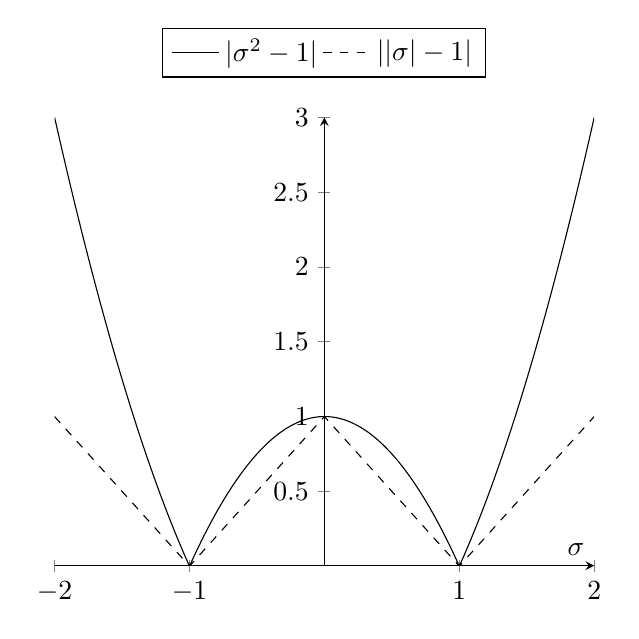
\begin{tikzpicture}
\begin{axis}[
    axis lines = center,
    xlabel = $\sigma$,
    %ylabel = {$f(x)$},
    legend style={at={(0.5,1.2)}, anchor=north,legend columns=-1}
]

\addplot [
    domain=-2:2, 
    samples=300, 
    color=black,
    ]
    {abs(x^2 -1)};
\addlegendentry{$|\sigma^2 -1|$}
\addplot [dashed,
    domain=-2:2, 
    samples=300, 
    color=black,
]
{abs(abs(x)-1)};
\addlegendentry{$||\sigma| -1|$}
\end{axis}
\end{tikzpicture}
\caption{Comparison between function $f$ (continuous line) and the distance from $S$ (dashed line) for $\X = \R$.}
    \label{fig:comparisons}
\end{figure}

\begin{figure}
\centering
\begin{tabular}{ccc}
\resizebox{.3\textwidth}{!}{
\begin{tikzpicture}
\begin{axis}[
    axis lines = center,
    xlabel = $\sigma$,
    %ylabel = {$f(x)$},
    legend style={at={(0.5,1.2)}, anchor=north,legend columns=-1}
]
\addplot [
    domain=-2:2, 
    samples=300, 
    color=black,
    ]
    {abs(x^2 -1)};
\addlegendentry{$|x^2 -1|$}
\end{axis}
\end{tikzpicture}}
&
\resizebox{.3\textwidth}{!}{
\begin{tikzpicture}
\begin{axis}[
    axis lines = center,
    xlabel = $\sigma$,
    %ylabel = {$f(x)$},
    legend style={at={(0.5,1.2)}, anchor=north,legend columns=-1}
]
\addplot [
    domain=-2:2, 
    samples=300, 
    color=black,
    ]
    {abs(x^2 -1) + x^2};
\addlegendentry{$|x^2 -1| + x^2$}
\end{axis}
\end{tikzpicture}
}
&
\resizebox{.3\textwidth}{!}{
\begin{tikzpicture}
\begin{axis}[
    axis lines = center,
    xlabel = $\sigma$,
    %ylabel = {$f(x)$},
    legend style={at={(0.5,1.2)}, anchor=north,legend columns=-1}
]
\addplot [
    domain=-2:2, 
    samples=300, 
    color=black,
    ]
    {abs(x^2 -1) + 2*x^2};
\addlegendentry{$|x^2 -1| + 2x^2$}
\end{axis}
\end{tikzpicture}
}
\end{tabular}
\caption{Comparison .}
    \label{fig:comparisons:2}
\end{figure}

In the previous part of this section, we proved that $f(x)$ can be a weakly convex function modelling the constraint related to the unit sphere in the feasibility problem between a sphere and a closed convex set $C$. To model the constraint with respect to the closed convex set $C$ we consider the differentiable function 
\begin{flalign}
\quad(\forall x \in \X)&& g(x) = \frac{\dist^2(x,C)}{2}, &&&
\end{flalign}
whose properties are summarised in the following lemma:

\begin{lemma}[{\cite[Corollary 12.30, Example 13.5]{Bauschke2017}}]\label{lem:dist}
    Let $C\subseteq \X$ be a convex set. Then 
    \begin{flalign}\label{eq:dist_func:diff_conv}
 \quad\left(\forall x \in \X\right) &&  
    \frac{\dist^2(x,C)}{2} = \frac{\|x\|^2}{2} - \left( \frac{\|\cdot\|^2}{2} + \iota_C\right)^*(x) &&&
\end{flalign}
{ where $x\mapsto  \left( \frac{\|\cdot\|^2}{2} + \iota_C\right)^*(x)$ denotes the Fenchel conjugate of function $x\mapsto  \left( \frac{\|\cdot\|^2}{2} + \iota_C\right)(x)$ {\cite[Definition 13.1]{Bauschke2017}}}. If in addition $C$ is closed, then function $\dist^2(\cdot,C)$ is Fréchet differentiable on $\X$ and 
    \begin{flalign}  \quad\left(\forall x \in \X\right) &&\nabla \frac{\dist^2(x,C)}{2} = x - \proj_C(x).&&&
    \end{flalign}
\end{lemma}
In particular, we highlight that the gradient of $x\mapsto\frac{\dist^2(x,C)}{2}$ is Lipschitz continuous as being the sum of two Lipschitz continuous functions.\\

The feasibility problem becomes
\begin{equation}
\label{FP}
\tag{Feasibility Problem}
\minimize{x\in\X}\, |\|x\|^2-1|+\frac{\dist^2(x,C)}{2}
\end{equation}
{where the objective function is non-convex. As a matter of facts, according to \autoref{lem:dist}, the problem can be recast as 
\begin{equation}
    \minimize{x\in\X}\, |\|x\|^2-1|+ \frac{\|x\|^2}{2} - \left( \frac{\|\cdot\|^2}{2} + \iota_C\right)^*(x).
\end{equation}
where function $x\mapsto |\|x\|^2-1|+ \frac{\|x\|^2}{2} $ is $1$-weakly convex by virtue of \autoref{lem:weak} and $x\mapsto- \left( \frac{\|\cdot\|^2}{2} + \iota_C\right)^*(x)$ is the negative of a conjugate function, hence it is concave since a Fenchel conjugate function is always convex \cite[Proposition 13.13]{Bauschke2017}).\\ }

Eventually, the sharpness of $f+g$, which is the core of our convergence result, holds by virtue of the following theorem, where $h_1 = f$ and $h_2 = g$.
\begin{theorem}\label{theo:sharpness 1}
    Let functions $\fonc{h_1,h_2}{\X}{\R}$ be proper and let the following assumptions be satisfied
    \setlist[enumerate,1]{label={(\roman*)}}
    \begin{enumerate} 
        \item The global minimiser set $S$ of $h_1+h_2$ is equal to (or contained in) $S_1\cap S_1$, if both nonempty, or $S\subset S_1$ where $S_1,S_2$ are the sets of the minimisers of $h_1$ and $h_2$ respectively.
        \item The optimal value of $h_1+h_2$ is zero, $v_{opt} =0$.
        \item $h_1(x)\geq 0, h_2(x) \geq 0$ for all $x$ in a neighborhood of $S$.
        \item $h_1$ is sharp with respect to $S$ locally or globally with constant $\mu>0$ and ${\inf_{x\in \X} h_1(x) =0}$.
    \end{enumerate}
    Then $h_1+h_2$ is locally (globally) sharp.
\end{theorem}
\begin{proof}
By \emph{(iv)} we have that there exists $\delta_1> 0$ such that 
\begin{flalign}
  \quad\left(\forall  x\in B(S,\delta_1)\right) && h_1(x) \geq \mu \dist (x,S).&&&
\end{flalign}
By $(iii)$ we know that there exists $\delta_2> 0$ such that for every $ x\in B(S,\delta_2)$ function $h_2$ is non-negative, hence by taking $\delta=\min\{\delta_1,\delta_2\}$ we have 
\begin{flalign}
\quad  \left(\forall  x\in B(S,\delta)\right) && h_1(x) + h_2(x) \geq \mu \dist (x,S).&&&
\end{flalign}
By $(i)$ and $(ii)$, the above inequality corresponds to the local sharpness of function $h_1+h_2$.
\end{proof}
% \begin{proposition}[{\cite[Section 3.3, Exercise 12]{borwein2006convex}}]
% Given a non-empty set $C\subset\H$ and define the distance function as 
% \begin{equation}
%     \label{eq:dist_func}
%  \left(\forall x \in \H\right)\qquad   \dist(x,C) = \inf_{y\in C} \|x-y\|.
% \end{equation}
% then the function $\dist^2(\cdot,C)$ can be expressed as a difference of convex functions
% \begin{equation}\label{eq:dist_func:diff_conv}
%  \left(\forall x \in \H\right)\qquad   
%     \dist^2(x,C) = \frac{\|x\|^2}{2} - \left( \frac{\|\cdot\|^2}{2} + \iota_C\right)^*(x).
% \end{equation}
% \end{proposition}
% In addition, let us suppose that $C$ is convex. Then the following holds:
% \begin{itemize}
%     \item function $\dist_C$ is convex and $\dist^*(\cdot,C)= \iota_{\{\|\cdot\|\leq 1\}} + \iota^*_C(\cdot)$;
%     \item if $C$ is closed then
%     \begin{equation}
%         \left(\forall x\in \H\setminus C\right)\qquad \nabla \dist(x,C) = \frac{1}{\dist(x,C)} (x - \proj_C(x))
%     \end{equation}
%     \begin{equation}
%         \left(\forall x \in\H\right)\qquad \nabla \frac{\dist^2(x,C)2}{2} = x - \proj_C(x).
%     \end{equation}
% \end{itemize}

% \lele{OBS In this infinite dimensional setting we can stress the fact that our setting applies in context where the KL setting is not sufficient. Let us say for example that we have an infinite intersection of closed convex sets. The resulting set is closed and convex, as required by our setting, but I don't know if it can satisfy the requirements of KL. (Look for reference)}
% \gio{The KL is usually proved in $\mathbb{R}^n$, but I don't know if there is a negative result in Hilbert.}\lele{there is a paper which works on KL in Hilbert - we cite it in the introduction - in the context of weakly convex functions!}

\section{Conclusions}

{In this paper we investigate the convergence properties of the exact and the inexact forward-backward (FB) algorithms for the minimisation of a function that is expressed as the sum of a weakly convex function and a convex function with Lipschitz continuous gradient. In the inexact case we inferred a convergence result that relies on the hypothesis that the accuracy level $\varepsilon> 0$ for the inexact proximal computation is kept constant throughout all the iterations. In order to carry out our analysis, we exploited the notion of proximal subdifferential and a calculus rule to compute the inexact proximal subdifferential of the sum two functions which controls the modulus of weak convexity $\rho$. It will be interesting in a future work to extend our results so as to take into account non-constant accuracy levels and non-convex smooth function.  } 
\paragraph{Acknowledgments}{This work has been supported by the ITN-ETN project TraDE-OPT funded by the European Union’s Horizon 2020 research and innovation programme under the Marie Skłodowska-Curie grant agreement No 861137.} {This work represents only the author’s view and the European Commission is not responsible for any use that may be made of the information it contains.}

\bibliographystyle{acm}
\bibliography{weak_convexity}
\appendix
\section{ Feasibility of the parameters} }\label{appendix:A}

\begin{lemma}
\label{lem:sequences}
    Given $\rho$, $\mu$ and $L_g$, we denote $\gamma := \max\{\rho,L_g\}$. Then for every $t\in\N$, the following choice of  $\varepsilon_t$, $\eta_t$ and $\alpha_t$,
      \begin{align}
\varepsilon_t &\in (0, \frac{\mu^2}{2\gamma}\sqrt{\sqrt{2}-1})\\
\tau_t&\in (\frac{2\gamma\varepsilon_t}{\mu^2}, \min\left\{ 1, \frac{\mu^2}{2\gamma\varepsilon_t}\sqrt{\sqrt{2}-1}\right\})\\
\Delta_\eta &=\frac{\mu^4\tau_t^2}{4\gamma_t^2} - \frac{\mu^2\tau_t}{\gamma_t}\left(\varepsilon_t +2\varepsilon_t\right) + \varepsilon_t^2\\
\underline{\eta}_t &= \left(\frac{1}{2} -   \frac{\gamma_t\varepsilon_t}{\mu^2\tau_t}\right) - \frac{\gamma_t}{\mu^2\tau_t} 
  \sqrt{\Delta_\eta}  \\
  \overline{\eta}_t &= \min\left\{1,  \left(\frac{1}{2} -   \frac{\gamma_t\varepsilon_t}{\mu^2\tau_t}\right) + \frac{\rho}{\mu^2\tau_t} 
  \sqrt{\Delta_\eta}\right\} \\
\eta_t &\in (\underline{\eta}_t,\overline{\eta}_t)\\
\alpha_t &= \tau_t (1-\eta_t)\frac{1}{\gamma_t}
  \end{align}
satisfies the inequalities \eqref{eq:cond:eta:1}, \eqref{eq:cond:eta:2} and \eqref{eq:cond:Lipsch} in \autoref{assu:conditions}.
% the following conditions:
% \begin{align}
% \label{eq:cond:eta:1}& 1-\alpha_t\rho - \eta_t > 0\\
% \label{eq:cond:eta:2}&\alpha_{t}\mu^2 \geq2\left(\varepsilon_{t}+\frac{\varepsilon_{t}}{\eta_{t}}\right)\left(\alpha_{t}\rho+\eta_{t}\right)\\
% \label{eq:cond:Lipsch} &\frac{1}{L_g}\geq \alpha_t.
% \end{align}
\end{lemma}

\begin{proof}
For condition \eqref{eq:cond:eta:1} to be valid, we need to have that for every $t\in \N$, $\eta_t \in (0,1)$. This implies the following condition on the stepsizes in $(\alpha_t)_{t \in \N}$
 \begin{equation}
     \frac{1}{\rho} >\frac{1-\eta_t}{\rho} >  \alpha_t 
 \end{equation}
 which combined with condition \eqref{eq:cond:Lipsch} implies that
 \begin{equation}
     \frac{2}{\alpha_t} > \rho + L_g,
 \end{equation}
 that is the condition ensuring inequality \eqref{eq:decrease} in \autoref{prop:eps:FB estimate g-convex}. \\
 
 On the other side, let us focus on condition \eqref{eq:cond:eta:2} which reads as
 \begin{align}
\alpha_{t}\mu^2 \geq2\left(\varepsilon_{t}+\frac{\varepsilon_{t}}{\eta_{t}}\right)\left(\alpha_{t}\rho+\eta_{t}\right)
 \end{align}
 If $\varepsilon_t=0$, then the condition is trivially satisified. Let us then consider the case when $\varepsilon_t>0$. From condition \eqref{eq:cond:eta:1} we have that $\alpha_t\rho + \eta_t <1$, so the LHS in \eqref{eq:cond:eta:2} satisfies
 \begin{equation}
     2\left( \varepsilon_t + \frac{\varepsilon_t}{\eta_t}\right)(\alpha_t \rho + \eta_t) < 2 \left(\varepsilon_t + \frac{\varepsilon_t}{\eta_t}\right)
 \end{equation}
 Let us set $\gamma = \max\left\{\rho, L_g\right\}$ and choose $\alpha_t = \tau_t (1-\eta_t)\frac{1}{\gamma}$ with $\tau_t \in (0,1) $ so that \eqref{eq:decrease}, \eqref{eq:cond:eta:1} and \eqref{eq:cond:Lipsch} are satisfied. In the following lines we will drop the dependency from $t$ for simplicity. For condition
 \eqref{eq:cond:eta:2} to be satisfied, it is sufficient that the following holds:
 \begin{equation}
   \eta\varepsilon + \varepsilon < \frac{\mu^2}{2} \alpha\eta  
 \end{equation}
Since $\alpha = \tau \frac{1-\eta}{\gamma}$ we have
 \begin{equation}
 \begin{aligned}
     &\eta\varepsilon + \varepsilon < \frac{\mu^2}{2}\tau \left(\frac{1-\eta}{\gamma}\right)\eta\\
     &\iff \frac{\mu^2}{2}\tau \frac{\eta}{\gamma} - \frac{\mu^2}{2}\tau \frac{\eta^2}{\gamma} - \eta \varepsilon - \varepsilon >0\\
     &\iff \frac{\mu^2}{2}\tau \frac{\eta^2}{\gamma} - \frac{\mu^2}{2}\tau \frac{\eta}{\gamma}  + \varepsilon\eta + \varepsilon <0\\
     &\iff \frac{\mu^2}{2}\tau \frac{\eta^2}{\gamma} + \left( \varepsilon - \frac{\mu^2\tau}{2\gamma}\right)\eta + \varepsilon < 0
     \end{aligned}
 \end{equation}
 This is a second order inequality in $\eta$ and the possible solutions lie inside an interval having extrema that are defined by
 \begin{equation}
     \eta_{1,2} = \frac{-\left( \varepsilon - \frac{\mu^2\tau}{2\gamma}\right)\pm \sqrt{\left( \varepsilon- \frac{\mu^2\tau}{2\gamma}\right)^2 - 4\left(\frac{\mu^2\tau}{2\gamma}\right)\varepsilon}}{\frac{\mu^2\tau}{\gamma}}
 \end{equation}
 In order to have positive values for $\eta_1$ and $\eta_2$ we need to require that $\tau$ is such that  
 \begin{equation}
 \begin{aligned}
     \left(\varepsilon -\frac{\mu^2\tau}{2\gamma}\right)\leq 0
     \iff \frac{2\gamma\varepsilon }{\mu^2}\leq \tau
     \end{aligned}
 \end{equation}
 and $\frac{2\gamma\varepsilon }{\mu^2}$ can be ensured to be smaller than 1 if by assumption we take $\varepsilon < \frac{\mu^2}{2\gamma}\sqrt{\sqrt{2}-1}$. On the other side, we also need to choose $\tau$ so that $\Delta_{\eta}$ is non-negative, that is
 \begin{equation}
 \begin{aligned}
    & \varepsilon^2 - 2\frac{\mu^2\tau}{2\gamma}\varepsilon + \frac{\mu^4\tau^2}{4\gamma^2} - \frac{4\mu^2\tau}{2\gamma}\varepsilon \geq 0\\
     &\iff  \frac{\mu^4\tau^2}{4\gamma^2} - \frac{\mu^2\tau}{\gamma}\left(\varepsilon +2\varepsilon\right) + \varepsilon^2\geq 0.
     \end{aligned}
 \end{equation}
We obtain a new inequality, this time in $\tau$, which is related to a second order equation having solutions that are defined by
 \begin{equation}
     \tau_{1,2} = \frac{\frac{\mu^2(3\varepsilon)}{\gamma} \pm \sqrt{\left(\frac{\mu^2}{\gamma}3\varepsilon\right)^2 - 4\varepsilon^2 \frac{\mu^4}{4\gamma^2}}}{2\varepsilon^2}
 \end{equation}
 and we have that $\frac{\mu^2(3\varepsilon)}{\gamma}>0$ and $\Delta_{\tau} = 9\frac{\mu^4}{\gamma^2}\varepsilon^2 - \frac{\mu^4}{\gamma^2}\varepsilon^2 = 8\frac{\mu^4}{\gamma^2}\varepsilon^2$. We then obtain
 \begin{equation}
 \begin{aligned}
     \tau \leq \tau_2 &= \frac{{\mu^2 3\varepsilon} - {2\sqrt{2}\mu^2\varepsilon}}{2\varepsilon^2\gamma} = \frac{{\mu^2\varepsilon}(\sqrt{2} -1) }{2\varepsilon^2\gamma} = \frac{{\mu^2} }{2\varepsilon\gamma}(\sqrt{2} -1)
     \end{aligned}
 \end{equation}
 In conclusion, to wrap up all the conditions we inferred on $\tau$ we have
 \begin{equation}
     \frac{2\gamma\varepsilon }{\mu^2}\leq \tau \leq \frac{{\mu^2} }{2\varepsilon\gamma}(\sqrt{2} -1)
 \end{equation}
where we know that the lower bound is strictly smaller than 1. In order to have admissible values for $\tau$ we need the following to hold
 \begin{equation}
 \begin{aligned}
     &\frac{2\gamma\varepsilon }{\mu^2}< \frac{{\mu^2}}{2\gamma\varepsilon}(\sqrt{2} - 1) \iff \varepsilon^2< \frac{{\mu^4}}{\gamma^2 4}(\sqrt{2} - 1) \iff \varepsilon< \frac{{\mu^2}}{2\gamma}\sqrt{\sqrt{2} - 1}
     \end{aligned}
 \end{equation}
which is satisfied by the hypothesis we mentioned above. In conclusion, we need to choose $\tau\in (\frac{2\gamma\varepsilon_t}{\mu^2}, \min\left\{ 1, \frac{\mu^2}{2\gamma\varepsilon_t}\sqrt{\sqrt{2}-1}\right\})$.

Coming back to $\eta$, the condition we found for $\tau$ allows to state that 
\begin{equation}
    \frac{-\left( \varepsilon - \frac{\mu^2\tau}{2\gamma}\right)- %\sqrt{\left( \varepsilon- \frac{\mu^2\tau}{2\gamma}\right)^2 - 4\left(\frac{\mu^2\tau}{2\gamma}\right)\varepsilon}
    \sqrt{\Delta_\eta}
    }{\frac{\mu^2\tau}{\gamma}} \leq \eta \leq \frac{-\left( \varepsilon - \frac{\mu^2\tau}{2\gamma}\right) + %\sqrt{\left( \varepsilon- \frac{\mu^2\tau}{2\gamma}\right)^2 - 4\left(\frac{\mu^2\tau}{2\gamma}\right)\varepsilon}
    \sqrt{\Delta_\eta}
    }{\frac{\mu^2\tau}{\gamma}}
\end{equation}
that is
\begin{equation}
\begin{aligned}
   \frac{\gamma}{\mu^2\tau}\left(\frac{\mu^2\tau}{2\gamma} - \varepsilon\right) - &\frac{\gamma}{\mu^2\tau} %\sqrt{\left( \varepsilon- \frac{\mu^2\tau}{2\gamma}\right)^2 - 4\left(\frac{\mu^2\tau}{2\gamma}\right)\varepsilon} 
   \sqrt{\Delta_\eta}
   \leq 
   \eta \leq \frac{\gamma}{\mu^2\tau}\left(\frac{\mu^2\tau}{2\gamma} - \varepsilon\right) + \frac{\gamma}{\mu^2\tau} %\sqrt{\left( \varepsilon- \frac{\mu^2\tau}{2\gamma}\right)^2 - 4\left(\frac{\mu^2\tau}{2\gamma}\right)\varepsilon}
   \sqrt{\Delta_\eta}
   \end{aligned}
\end{equation}
\begin{equation}
\begin{aligned}
  \left(\frac{1}{2} -   \frac{\gamma\varepsilon}{\mu^2\tau}\right) - &\frac{\gamma}{\mu^2\tau} %\sqrt{\left( \varepsilon- \frac{\mu^2\tau}{2\gamma}\right)^2 - 4\left(\frac{\mu^2\tau}{2\gamma}\right)\varepsilon} 
  \sqrt{\Delta_\eta}
   \leq
   \eta \leq \left(\frac{1}{2} -   \frac{\gamma\varepsilon}{\mu^2\tau}\right) + \frac{\gamma}{\mu^2\tau} %\sqrt{\left( \varepsilon- \frac{\mu^2\tau}{2\gamma}\right)^2 - 4\left(\frac{\mu^2\tau}{2\gamma}\right)\varepsilon}
   \sqrt{\Delta_\eta}
   \end{aligned}
\end{equation}
and we have $0<\left(\frac{1}{2} -   \frac{\gamma\varepsilon}{\mu^2\tau}\right)\leq 1$. We conclude that for the choice of $\tau$ we found above, we have $[\eta_1,\eta_2]\cap (0,1) \neq \emptyset$ and we can define 
\begin{align}\underline{\eta} &= \left(\frac{1}{2} -   \frac{\gamma\varepsilon}{\mu^2\tau}\right) - \frac{\gamma}{\mu^2\tau} 
  \sqrt{\Delta_\eta} = \eta_1 \\
  \overline{\eta} &= \min\left\{1,  \left(\frac{1}{2} -   \frac{\gamma\varepsilon}{\mu^2\tau}\right) + \frac{\rho}{\mu^2\tau} 
  \sqrt{\Delta_\eta}\right\} = \min\{1,\eta_2\}
  \end{align}
  and choose $\eta \in (\underline{\eta},\overline{\eta})\subset (0,1)$. \\
  
  To sum up, in order to satisfy the conditions \eqref{eq:cond:eta:1}, \eqref{eq:cond:eta:2} and \eqref{eq:cond:Lipsch}, we need to have for every $t\in\N$
  \begin{align}
  \gamma &= \max\{\rho,L_g\}\\
\varepsilon_t &\in (0, \frac{\mu^2}{2\gamma}\sqrt{\sqrt{2}-1})\\
\tau_t&\in (\frac{2\gamma\varepsilon_t}{\mu^2}, \min\left\{ 1, \frac{\mu^2}{2\gamma\varepsilon_t}\sqrt{\sqrt{2}-1}\right\})\\
\eta_t &\in (\underline{\eta}_t,\overline{\eta}_t)\\
\alpha_t &= \tau_t (1-\eta_t)\frac{1}{\gamma}
  \end{align}

%   If for such a choice $\eta$ we have to take $\alpha = \frac{1}{L_g}$, we have
%  \begin{equation}
%      \begin{aligned}
%       &\eta\varepsilon+\varepsilon < \frac{\mu^2}{2} \frac{1}{L_g}\eta\\
%       &\iff \eta\left(\varepsilon - \frac{\mu^2}{2} \frac{1}{L_g}\right) < -\varepsilon\\
%       &\iff \eta > \frac{\varepsilon}{\frac{\mu^2}{2} \frac{1}{L_g} - \varepsilon}
%      \end{aligned}
%  \end{equation}
%  and the lower bound satisfies
%  \begin{equation}
%  \begin{aligned}
%      &\frac{\varepsilon}{\frac{\mu^2}{2} \frac{1}{L_g} - \varepsilon} <1\\
%      &\iff 2\varepsilon < \frac{\mu^2}{2L_g}
%  \end{aligned}
%  \end{equation}
%  which can be ensured for some $\tau \in (0,1)$ if we assume from the beginning that $\varepsilon < \frac{\mu^2}{4L_g}$.
 

%  Notice that in the three inequalities above, the RHS is positive by virtue of the upper bound for $\varepsilon$ defined in \autoref{prop:eps:statpoint}.
\end{proof}
\section{Discriminant from \autoref{lem:inthetube:const}} \label{sec:appendix:discriminant}
Let us calculate the discriminant related to inequality \eqref{eq:ineq:discriminant}, in order to define the existence of solutions.% In fact, for varying parameters, we can obtain the same result for one instance $t\in\N$:
\begin{align}\label{eq:discriminant:plus}
&\Delta^+  =\alpha ^{2}\mu^{2}+\left(1-\alpha \rho-\eta \right)\left(\left(\frac{\alpha \mu+\sqrt{\alpha ^{2}\mu^{2}-2\alpha \left(\varepsilon +\frac{\varepsilon }{\eta }\right)\left(\alpha \rho+\eta \right)}}{\alpha \rho+\eta }\right)^{2}+2\alpha \left(\varepsilon +\frac{\varepsilon }{\eta }\right)\right)\\
 & =\frac{\alpha ^{2}\mu^{2}\left(\alpha \rho+\eta \right)^{2}}{\left(\alpha \rho+\eta \right)^{2}}\\
 & +\frac{\left(1-\alpha \rho-\eta \right)\left(\left(\alpha \mu+\sqrt{\alpha ^{2}\mu^{2}-2\alpha \left(\varepsilon +\frac{\varepsilon }{\eta }\right)\left(\alpha \rho+\eta \right)}\right)^{2}+2\alpha \left(\varepsilon +\frac{\varepsilon }{\eta }\right)\left(\alpha \rho+\eta \right)^{2}\right)}{\left(\alpha \rho+\eta \right)^{2}} \\
 & = \frac{\alpha ^{2}\mu^{2} \left(\alpha \rho+\eta \right)^{2}+2\alpha ^{2}\mu^{2}\left(1-\alpha \rho-\eta \right)}{\left(\alpha \rho+\eta \right)^{2}} -\frac{2\alpha \left(\varepsilon +\frac{\varepsilon }{\eta }\right)\left(\alpha \rho+\eta \right)\left(1-\alpha \rho-\eta \right)}{\left(\alpha \rho+\eta \right)^{2}}\\
 &+\frac{2\alpha \mu \sqrt{\alpha ^{2}\mu^{2} -2\alpha \left(\varepsilon +\frac{\varepsilon }{\eta }\right)\left(\alpha \rho+\eta \right)} \left(1-\alpha \rho-\eta \right)}{\left(\alpha \rho+\eta \right)^{2}}\\ &+\frac{2\alpha \left(\varepsilon +\frac{\varepsilon }{\eta }\right)\left(\alpha \rho+\eta \right)^{2}\left(1-\alpha \rho-\eta \right)}{\left(\alpha \rho+\eta \right)^{2}}\\
 & =\frac{\alpha ^{2}\mu^{2}+\left(1-\alpha \rho-\eta \right)^{2}\left(\alpha ^{2}\mu^{2}-2\alpha \left(\varepsilon +\frac{\varepsilon }{\eta }\right)\left(\alpha \rho+\eta \right)\right)}{\left(\alpha \rho+\eta \right)^{2}}\\
 & +\frac{2\alpha \mu\left(1-\alpha \rho-\eta \right)\sqrt{\alpha ^{2}\mu^{2}-2\alpha \left(\varepsilon +\frac{\varepsilon }{\eta }\right)\left(\alpha \rho+\eta \right)}}{\left(\alpha \rho+\eta \right)^{2}} \\
 & =\left(\frac{\alpha \mu+\left(1-\alpha \rho-\eta \right)\sqrt{\alpha ^{2}\mu^{2}-2\alpha \left(\varepsilon +\frac{\varepsilon }{\eta }\right)\left(\alpha \rho+\eta \right)}}{\alpha \rho+\eta }\right)^{2}.
\end{align}
Let us calculate the upper bound in equation \eqref{eq:discriminant}
\begin{equation}\label{eq:appendix:discriminant}
    \begin{aligned}
&\frac{-\alpha \mu+\sqrt{\Delta^+}}{1-\alpha \rho-\eta }=\\
& \qquad= 
\frac{-\alpha \mu+\frac{\alpha \mu+\left(1-\alpha \rho-\eta \right)\sqrt{\alpha ^{2}\mu^{2}-2\alpha \left(\varepsilon +\frac{\varepsilon }{\eta }\right)\left(\alpha \rho+\eta \right)}}{\alpha \rho+\eta }}{1-\alpha \rho-\eta }
\\
& \qquad= 
\frac{-\alpha \mu(\alpha \rho + \eta )+{\alpha \mu+\left(1-\alpha \rho-\eta \right)\sqrt{\alpha ^{2}\mu^{2}-2\alpha \left(\varepsilon +\frac{\varepsilon }{\eta }\right)\left(\alpha \rho+\eta \right)}}{}}{\left(1-\alpha \rho-\eta \right) \left( \alpha \rho+\eta \right)}
\\
&\qquad=\frac{\alpha \mu\left(1-\alpha \rho-\eta \right)+\left(1-\alpha \rho-\eta \right)\sqrt{\alpha ^{2}\mu^{2}-2\alpha \left(\varepsilon +\frac{\varepsilon }{\eta }\right)\left(\alpha \rho+\eta \right)}}{\left(1-\alpha \rho-\eta \right)\left(\alpha \rho+\eta \right)}\\
&\qquad = \frac{\alpha \mu+\sqrt{\alpha ^{2}\mu^{2}-2\alpha \left(\varepsilon +\frac{\varepsilon }{\eta }\right)\left(\alpha \rho+\eta \right)}}{\left(\alpha \rho+\eta \right)}.
\end{aligned}
\end{equation}

{
Let us calculate the discriminant ($\Delta^-$) and the upper bound for the second part of the statement, that is when ${\dist(x_{t_0},S) < E^-}$.
\begin{equation}\label{eq:discriminant:minus}
\begin{aligned}
&\Delta^-  =\alpha ^{2}\mu^{2}+\left(1-\alpha \rho-\eta \right)\left(\left(\frac{\alpha \mu-\sqrt{\alpha ^{2}\mu^{2}-2\alpha \left(\varepsilon +\frac{\varepsilon }{\eta }\right)\left(\alpha \rho+\eta \right)}}{\alpha \rho+\eta }\right)^{2}+2\alpha \left(\varepsilon +\frac{\varepsilon }{\eta }\right)\right)\\
 & =\frac{\alpha ^{2}\mu^{2}\left(\alpha \rho+\eta \right)^{2}}{\left(\alpha \rho+\eta \right)^{2}}\\
 & +\frac{\left(1-\alpha \rho-\eta \right)\left(\left(\alpha \mu{\color{blue} -}\sqrt{\alpha ^{2}\mu^{2}-2\alpha \left(\varepsilon +\frac{\varepsilon }{\eta }\right)\left(\alpha \rho+\eta \right)}\right)^{2}+2\alpha \left(\varepsilon +\frac{\varepsilon }{\eta }\right)\left(\alpha \rho+\eta \right)^{2}\right)}{\left(\alpha \rho+\eta \right)^{2}} \\
 & = \frac{\alpha ^{2}\mu^{2} \left(\alpha \rho+\eta \right)^{2}+2\alpha ^{2}\mu^{2}\left(1-\alpha \rho-\eta \right)}{\left(\alpha \rho+\eta \right)^{2}} -\frac{2\alpha \left(\varepsilon +\frac{\varepsilon }{\eta }\right)\left(\alpha \rho+\eta \right)\left(1-\alpha \rho-\eta \right)}{\left(\alpha \rho+\eta \right)^{2}}\\
 &-\frac{2\alpha \mu \sqrt{\alpha ^{2}\mu^{2} -2\alpha \left(\varepsilon +\frac{\varepsilon }{\eta }\right)\left(\alpha \rho+\eta \right)} \left(1-\alpha \rho-\eta \right)}{\left(\alpha \rho+\eta \right)^{2}}\\ &+\frac{2\alpha \left(\varepsilon +\frac{\varepsilon }{\eta }\right)\left(\alpha \rho+\eta \right)^{2}\left(1-\alpha \rho-\eta \right)}{\left(\alpha \rho+\eta \right)^{2}}\\
 & =\frac{\alpha ^{2}\mu^{2}+\left(1-\alpha \rho-\eta \right)^{2}\left(\alpha ^{2}\mu^{2}-2\alpha \left(\varepsilon +\frac{\varepsilon }{\eta }\right)\left(\alpha \rho+\eta \right)\right)}{\left(\alpha \rho+\eta \right)^{2}}\\
 & -\frac{2\alpha \mu\left(1-\alpha \rho-\eta \right)\sqrt{\alpha ^{2}\mu^{2}-2\alpha \left(\varepsilon +\frac{\varepsilon }{\eta }\right)\left(\alpha \rho+\eta \right)}}{\left(\alpha \rho+\eta \right)^{2}} \\
 & =\left(\frac{\alpha \mu{\color{blue} -}\left(1-\alpha \rho-\eta \right)\sqrt{\alpha ^{2}\mu^{2}-2\alpha \left(\varepsilon +\frac{\varepsilon }{\eta }\right)\left(\alpha \rho+\eta \right)}}{\alpha \rho+\eta }\right)^{2}.
\end{aligned}
\end{equation}
Let us calculate the upper bound 
\begin{equation}\label{eq:appendix:discriminant:minus}
    \begin{aligned}
&\frac{-\alpha \mu+\sqrt{\Delta^-}}{1-\alpha \rho-\eta }=\\
& \qquad= 
\frac{-\alpha \mu+\frac{\alpha \mu{ \color{blue}-}\left(1-\alpha \rho-\eta \right)\sqrt{\alpha ^{2}\mu^{2}-2\alpha \left(\varepsilon +\frac{\varepsilon }{\eta }\right)\left(\alpha \rho+\eta \right)}}{\alpha \rho+\eta }}{1-\alpha \rho-\eta }
\\
& \qquad= 
\frac{-\alpha \mu(\alpha \rho + \eta )+{\alpha \mu-\left(1-\alpha \rho-\eta \right)\sqrt{\alpha ^{2}\mu^{2}-2\alpha \left(\varepsilon +\frac{\varepsilon }{\eta }\right)\left(\alpha \rho+\eta \right)}}{}}{\left(1-\alpha \rho-\eta \right) \left( \alpha \rho+\eta \right)}
\\
&\qquad=\frac{\alpha \mu\left(1-\alpha \rho-\eta \right){\color{blue} -}\left(1-\alpha \rho-\eta \right)\sqrt{\alpha ^{2}\mu^{2}-2\alpha \left(\varepsilon +\frac{\varepsilon }{\eta }\right)\left(\alpha \rho+\eta \right)}}{\left(1-\alpha \rho-\eta \right)\left(\alpha \rho+\eta \right)}\\
&\qquad = \frac{\alpha \mu -\sqrt{\alpha ^{2}\mu^{2}-2\alpha \left(\varepsilon +\frac{\varepsilon }{\eta }\right)\left(\alpha \rho+\eta \right)}}{\left(\alpha \rho+\eta \right)}.
\end{aligned}
\end{equation}
}
\end{document}
